\documentclass[twoside]{book}

% Packages required by doxygen
\usepackage{fixltx2e}
\usepackage{calc}
\usepackage{doxygen}
\usepackage[export]{adjustbox} % also loads graphicx
\usepackage{graphicx}
\usepackage[utf8]{inputenc}
\usepackage{makeidx}
\usepackage{multicol}
\usepackage{multirow}
\PassOptionsToPackage{warn}{textcomp}
\usepackage{textcomp}
\usepackage[nointegrals]{wasysym}
\usepackage[table]{xcolor}

% Font selection
\usepackage[T1]{fontenc}
\usepackage[scaled=.90]{helvet}
\usepackage{courier}
\usepackage{amssymb}
\usepackage{sectsty}
\renewcommand{\familydefault}{\sfdefault}
\allsectionsfont{%
  \fontseries{bc}\selectfont%
  \color{darkgray}%
}
\renewcommand{\DoxyLabelFont}{%
  \fontseries{bc}\selectfont%
  \color{darkgray}%
}
\newcommand{\+}{\discretionary{\mbox{\scriptsize$\hookleftarrow$}}{}{}}

% Page & text layout
\usepackage{geometry}
\geometry{%
  a4paper,%
  top=2.5cm,%
  bottom=2.5cm,%
  left=2.5cm,%
  right=2.5cm%
}
\tolerance=750
\hfuzz=15pt
\hbadness=750
\setlength{\emergencystretch}{15pt}
\setlength{\parindent}{0cm}
\setlength{\parskip}{3ex plus 2ex minus 2ex}
\makeatletter
\renewcommand{\paragraph}{%
  \@startsection{paragraph}{4}{0ex}{-1.0ex}{1.0ex}{%
    \normalfont\normalsize\bfseries\SS@parafont%
  }%
}
\renewcommand{\subparagraph}{%
  \@startsection{subparagraph}{5}{0ex}{-1.0ex}{1.0ex}{%
    \normalfont\normalsize\bfseries\SS@subparafont%
  }%
}
\makeatother

% Headers & footers
\usepackage{fancyhdr}
\pagestyle{fancyplain}
\fancyhead[LE]{\fancyplain{}{\bfseries\thepage}}
\fancyhead[CE]{\fancyplain{}{}}
\fancyhead[RE]{\fancyplain{}{\bfseries\leftmark}}
\fancyhead[LO]{\fancyplain{}{\bfseries\rightmark}}
\fancyhead[CO]{\fancyplain{}{}}
\fancyhead[RO]{\fancyplain{}{\bfseries\thepage}}
\fancyfoot[LE]{\fancyplain{}{}}
\fancyfoot[CE]{\fancyplain{}{}}
\fancyfoot[RE]{\fancyplain{}{\bfseries\scriptsize Generated by Doxygen }}
\fancyfoot[LO]{\fancyplain{}{\bfseries\scriptsize Generated by Doxygen }}
\fancyfoot[CO]{\fancyplain{}{}}
\fancyfoot[RO]{\fancyplain{}{}}
\renewcommand{\footrulewidth}{0.4pt}
\renewcommand{\chaptermark}[1]{%
  \markboth{#1}{}%
}
\renewcommand{\sectionmark}[1]{%
  \markright{\thesection\ #1}%
}

% Indices & bibliography
\usepackage{natbib}
\usepackage[titles]{tocloft}
\setcounter{tocdepth}{3}
\setcounter{secnumdepth}{5}
\makeindex

% Hyperlinks (required, but should be loaded last)
\usepackage{ifpdf}
\ifpdf
  \usepackage[pdftex,pagebackref=true]{hyperref}
\else
  \usepackage[ps2pdf,pagebackref=true]{hyperref}
\fi
\hypersetup{%
  colorlinks=true,%
  linkcolor=blue,%
  citecolor=blue,%
  unicode%
}

% Custom commands
\newcommand{\clearemptydoublepage}{%
  \newpage{\pagestyle{empty}\cleardoublepage}%
}

\usepackage{caption}
\captionsetup{labelsep=space,justification=centering,font={bf},singlelinecheck=off,skip=4pt,position=top}

%===== C O N T E N T S =====

\begin{document}

% Titlepage & ToC
\hypersetup{pageanchor=false,
             bookmarksnumbered=true,
             pdfencoding=unicode
            }
\pagenumbering{alph}
\begin{titlepage}
\vspace*{7cm}
\begin{center}%
{\Large Listen\+App \\[1ex]\large 2.\+0 }\\
\vspace*{1cm}
{\large Generated by Doxygen 1.8.14}\\
\end{center}
\end{titlepage}
\clearemptydoublepage
\pagenumbering{roman}
\tableofcontents
\clearemptydoublepage
\pagenumbering{arabic}
\hypersetup{pageanchor=true}

%--- Begin generated contents ---
\chapter{Listen\+App Documentation}
\label{index}\hypertarget{index}{}\hypertarget{index_zero}{}\section{Prerequisites}\label{index_zero}
To run Listen\+App, you need
\begin{DoxyItemize}
\item Visual Studio C\# developing environment
\item Windows 10 dektop with Cortana. Some functionalities might be available in Windows 8.\+1+ as well as in Windows Phone Versions, I\textquotesingle{}m not guaranteeing that however, since it\textquotesingle{}s not tested.
\item to be registered as a user in the webform (the userename and password is needed for most methods, except when running in Mock-\/\+Mode)
\item there are a number of other registrations that the App needs and that I have already provided in the background. If I will ever shut down those online services, you will have to create those on your own as follows\+:
\begin{DoxyEnumerate}
\item Microsoft Developer Account
\item L\+U\+IS Account
\item Azure Account
\item Bot Developer Account
\item Cortana Developer Account -\/microphone permission on your device is preferable. Otherwise you will be only able to run the App in text-\/mode.
\end{DoxyEnumerate}
\end{DoxyItemize}\hypertarget{index_first}{}\section{Functionality}\label{index_first}
Listen\+App is the main component of \mbox{\hyperlink{namespace_listen_to_me}{Listen\+To\+Me}} project. It contains a visual representation of the online form E\+SF and an text or speech input line. Input is evaluated by sending the phrases to the online Service L\+U\+IS or to the online Service Bot with Send\+Message(), and then evaluating the response in dertermine\+Response(). The available, enabled input fields at the App as well as radio buttons and dropdown lists are referenced in a Hashtable with their labels as keys. If the App recognizes a match with one of the labels in the App, it will fill in the recognised field value in the phrase into that very field. If it is not sure -\/ sometimes there are several inputs with the same label -\/ it will ask the user for disambiguation. As it is, Listen\+App can\textquotesingle{}t upload the data back to the online form. There is a in GO written component formularinstanzservice that has to be addressed for that and I haven\textquotesingle{}t yet figured out how to do that.\hypertarget{index_second}{}\section{Pecularities}\label{index_second}
The W\+CF Service is implemented in Factory Pattern. The facory is able to produce either in Mock-\/\+Mode or in Real-\/\+Mode output. Mock-\/\+Mode is independant from the availability of the form to be parsed. It reads from a text file called Sections.\+json which is included in the project. Real-\/\+Mode however, does call the domain of the webform to archieve the same purpose.

If the app is throwing a C\+O\+M\+Exception, the problem is that it can\textquotesingle{}t find the W\+CF Service on which it depends. The workaround for this is to delete the service reference in the app, rebuild the W\+CF Service project and create a new service reference to the Service1.\+svc of W\+CF Service project in this app.\hypertarget{index_third}{}\section{To\+Dos}\label{index_third}

\begin{DoxyItemize}
\item Die Buttons zum Hinzufügen von Tabellenzeilen bei den favorisierten Bildungsanbietern sind nicht ohne weiteres darstellbar. Aufgrund der Tabellenstruktur im H\+T\+M\+L-\/\+Code, die sehr schwer mit X\+P\+A\+TH auslesbar sein wird, sind die Feldbeschriftungen zugeteilt.
\item Testen, ob cut\+Leading\+Numbers in W\+C\+F\+Service tatsächlich die führenden Nummern aus den Feldern Gründungsdatum ect. schneidet. Wichtig für Bot.
\item Der Selenium\+Browser von W\+CF Service wird nicht beendet
\item Das Formular in Polnisch und Englisch abrufen -\/$>$ neue Dummyelemente generieren
\item Der W\+CF Service ist extrem spezifisch auf das vorliegende Formular hörig. Da er als Grundlage die Html-\/\+Seite parst, hat er keinen zugriff auf die Dahinterliegende Logik, zum Beispiel die Angular-\/\+Direktiven, die dafür sorgen, dass in einem bestimmten Feld eine Summe eingetragen wird, sobald ein anderes ausgefüllt ist. Die Darstellung der dynamischen Inhalte kann er nicht abbilden, z.\+B. Berechnungen, wieviele Zeichen noch übrig sind, Fehlermeldungen und Button-\/\+Aktionen.
\item Ressource Binding läuft für die Checkboxes und Radio\+Buttons nicht glatt
\item up\+Load\+To\+Jason() wirft
\end{DoxyItemize}


\begin{DoxyCode}
StatusCode: 400, ReasonPhrase: 'BadArgument', Version: 1.1, Content: System.Net.Http.StreamContent,
       Headers:
\{
  Request-Context: appId=cid-v1:26a3540d-a02a-4998-a060-715488fd769b
  Strict-Transport-Security: max-age=31536000; includeSubDomains; preload
  Request-Id: c60c9469-68e3-40a5-bb8e-beaa61870875
  Cache-Control: no-store, proxy-revalidate, no-cache, max-age=0, private
  Date: Thu, 14 Dec 2017 07:51:09 GMT
  X-Frame-Options: SAMEORIGIN
  X-Powered-By: ASP.NET
  X-Content-Type-Options: nosniff
  Pragma: no-cache
  Apim-Request-Id: c60c9469-68e3-40a5-bb8e-beaa61870875
  Content-Length: 152
  Content-Type: application/json; charset=utf-8
\}
\end{DoxyCode}



\begin{DoxyItemize}
\item das Codesnippet in den Bot einbauen, das die Cortana information zur email und username abruft, möglich?
\item ändere meine $<$\+Seite$>$ läuft nicht für Seiten, die aus mehr als einem Wort bestehen zum Beispiel \char`\"{}Ändere Listen\+To\+Me Registereintragungen\char`\"{} läuft, nicht aber \char`\"{}ändere listentome rggistereintraggunggen\char`\"{} und \char`\"{}Ändere Listen\+To\+Me Sitz des Antragsstellers\char`\"{}
\end{DoxyItemize}

Kann ich nur zuhause/mit Botframework\+Emulator debuggen\+:
\begin{DoxyItemize}
\item die längeren Eingaben funktionieren nicht mehr wenn Cortana auf U\+SA eingestellt ist \char`\"{}\+Ich möchte die Unternehmensangaben im E\+S\+F\+\_\+2 Formular ausfüllen, z.\+B.\char`\"{}
\item dateiupload und helpdialog stürtzen ab 
\end{DoxyItemize}
\chapter{Namespace Index}
\section{Packages}
Here are the packages with brief descriptions (if available)\+:\begin{DoxyCompactList}
\item\contentsline{section}{\hyperlink{namespace_listen_to_me}{Listen\+To\+Me} }{\pageref{namespace_listen_to_me}}{}
\end{DoxyCompactList}

\chapter{Hierarchical Index}
\section{Class Hierarchy}
This inheritance list is sorted roughly, but not completely, alphabetically\+:\begin{DoxyCompactList}
\item \contentsline{section}{Class\+Library.\+model.\+Bot\+Json}{\pageref{class_class_library_1_1model_1_1_bot_json}}{}
\item Dictionary\begin{DoxyCompactList}
\item \contentsline{section}{Class\+Library.\+model.\+Message}{\pageref{class_class_library_1_1model_1_1_message}}{}
\item \contentsline{section}{Class\+Library.\+model.\+Node}{\pageref{class_class_library_1_1model_1_1_node}}{}
\end{DoxyCompactList}
\item \contentsline{section}{Class\+Library.\+model.\+Form}{\pageref{class_class_library_1_1model_1_1_form}}{}
\item I\+Notify\+Property\+Changed\begin{DoxyCompactList}
\item \contentsline{section}{Class\+Library.\+model.\+Element}{\pageref{class_class_library_1_1model_1_1_element}}{}
\end{DoxyCompactList}
\item \contentsline{section}{Class\+Library.\+model.\+Property}{\pageref{class_class_library_1_1model_1_1_property}}{}
\item \contentsline{section}{Class\+Library.\+model.\+Section}{\pageref{class_class_library_1_1model_1_1_section}}{}
\end{DoxyCompactList}

\chapter{Class Index}
\section{Class List}
Here are the classes, structs, unions and interfaces with brief descriptions\+:\begin{DoxyCompactList}
\item\contentsline{section}{\hyperlink{class_listen_to_me_1_1_app}{Listen\+To\+Me.\+App} \\*contains application specific methods for starting the application. Initializations and state-\/related actions are includes. }{\pageref{class_listen_to_me_1_1_app}}{}
\item\contentsline{section}{\hyperlink{class_listen_to_me_1_1_cortana_model_methods}{Listen\+To\+Me.\+Cortana\+Model\+Methods} \\*Contains methods that update the cortana voice command definition file to make it more dynamic. Note\+: This doesn\textquotesingle{}t work as intendet, because phrase lists are only allowing one word entries and the form headings are mostly more than one word long. }{\pageref{class_listen_to_me_1_1_cortana_model_methods}}{}
\item\contentsline{section}{\hyperlink{class_listen_to_me_1_1_common_1_1_date_time_offset_converter}{Listen\+To\+Me.\+Common.\+Date\+Time\+Offset\+Converter} \\*Convert a Date\+Time to a Date\+Time\+Offset for use by a Date\+Picker, and back to allow for two-\/day data-\/binding. }{\pageref{class_listen_to_me_1_1_common_1_1_date_time_offset_converter}}{}
\item\contentsline{section}{\hyperlink{class_listen_to_me_1_1_view_1_1_disambiguate_view}{Listen\+To\+Me.\+View.\+Disambiguate\+View} \\*}{\pageref{class_listen_to_me_1_1_view_1_1_disambiguate_view}}{}
\item\contentsline{section}{\hyperlink{class_listen_to_me_1_1_dynamic_page}{Listen\+To\+Me.\+Dynamic\+Page} \\*This is a page that can be dynamically filled in \hyperlink{class_listen_to_me_1_1_main_page}{Main\+Page}. It is used to display the components that the wcf service finds per section on the form }{\pageref{class_listen_to_me_1_1_dynamic_page}}{}
\item\contentsline{section}{\hyperlink{class_listen_to_me_1_1_model_1_1_entity}{Listen\+To\+Me.\+Model.\+Entity} \\*subclass of Root\+Object. Note\+: these classes were easily pasted in C\# using the visual studio tools for converting J\+S\+ON }{\pageref{class_listen_to_me_1_1_model_1_1_entity}}{}
\item\contentsline{section}{\hyperlink{class_listen_to_me_1_1_model_1_1_form}{Listen\+To\+Me.\+Model.\+Form} \\*able to store Sections of the form. $<$reference$>$Adventure\+Works in U\+WP sample projects at github$<$/reference$>$ /summary$>$ }{\pageref{class_listen_to_me_1_1_model_1_1_form}}{}
\item\contentsline{section}{\hyperlink{interface_listen_to_me_1_1_common_1_1_i_navigation_service}{Listen\+To\+Me.\+Common.\+I\+Navigation\+Service} \\*Navigation service interface, allows a test implementation to be substituted in its place. }{\pageref{interface_listen_to_me_1_1_common_1_1_i_navigation_service}}{}
\item\contentsline{section}{\hyperlink{class_listen_to_me_1_1_model_1_1_intent}{Listen\+To\+Me.\+Model.\+Intent} \\*subclass of Root\+Object. Note\+: these classes were easily pasted in C\# using the visual studio tools for converting J\+S\+ON }{\pageref{class_listen_to_me_1_1_model_1_1_intent}}{}
\item\contentsline{section}{\hyperlink{class_listen_to_me_1_1_model_1_1_listen_to_me_voice_command}{Listen\+To\+Me.\+Model.\+Listen\+To\+Me\+Voice\+Command} \\*class for storing arguments. used by \hyperlink{class_listen_to_me_1_1_app}{App} to bind launch arguments (e.\+g. from Cortana) }{\pageref{class_listen_to_me_1_1_model_1_1_listen_to_me_voice_command}}{}
\item\contentsline{section}{\hyperlink{class_listen_to_me_1_1_common_1_1_load_state_event_args}{Listen\+To\+Me.\+Common.\+Load\+State\+Event\+Args} \\*Class used to hold the event data required when a page attempts to load state. }{\pageref{class_listen_to_me_1_1_common_1_1_load_state_event_args}}{}
\item\contentsline{section}{\hyperlink{class_listen_to_me_1_1_login_page}{Listen\+To\+Me.\+Login\+Page} \\*retrieves and stores login Information in a password vault to\+Do\+: use this for direct\+Line secret as well }{\pageref{class_listen_to_me_1_1_login_page}}{}
\item\contentsline{section}{\hyperlink{class_listen_to_me_1_1_main_page}{Listen\+To\+Me.\+Main\+Page} \\*contains the navigation buttons of the app as well as the speech input field }{\pageref{class_listen_to_me_1_1_main_page}}{}
\item\contentsline{section}{\hyperlink{class_listen_to_me_1_1_common_1_1_navigation_helper}{Listen\+To\+Me.\+Common.\+Navigation\+Helper} \\*aids in navigation between pages. It manages the backstack and integrates Suspension\+Manager to handle process lifetime management and state management when navigating between pages. }{\pageref{class_listen_to_me_1_1_common_1_1_navigation_helper}}{}
\item\contentsline{section}{\hyperlink{class_listen_to_me_1_1_common_1_1_navigation_service}{Listen\+To\+Me.\+Common.\+Navigation\+Service} \\*Navigation system that decouples the \hyperlink{namespace_listen_to_me_1_1_view}{View} \hyperlink{namespace_listen_to_me_1_1_model}{Model} from knowledge of the \hyperlink{namespace_listen_to_me_1_1_view}{View} for navigation purposes. This class can be replaced with a simple mock implementation for test purposes. }{\pageref{class_listen_to_me_1_1_common_1_1_navigation_service}}{}
\item\contentsline{section}{\hyperlink{class_listen_to_me_1_1_model_1_1_proxy}{Listen\+To\+Me.\+Model.\+Proxy} \\*queries L\+U\+I\+Sbot\+Ai with techniques of Collin Blake from \href{https://www.youtube.com/watch?v=ziLkj4PmcCE}{\tt https\+://www.\+youtube.\+com/watch?v=zi\+Lkj4\+Pmc\+CE} }{\pageref{class_listen_to_me_1_1_model_1_1_proxy}}{}
\item\contentsline{section}{\hyperlink{class_listen_to_me_1_1_common_1_1_root_frame_navigation_helper}{Listen\+To\+Me.\+Common.\+Root\+Frame\+Navigation\+Helper} \\*registers for standard mouse and keyboard shortcuts used to go back and forward. There should be only one instance of this class per view, and it should be associated with the root frame. }{\pageref{class_listen_to_me_1_1_common_1_1_root_frame_navigation_helper}}{}
\item\contentsline{section}{\hyperlink{class_listen_to_me_1_1_model_1_1_rootobject}{Listen\+To\+Me.\+Model.\+Rootobject} \\*models the default L\+U\+IS Http-\/answer which consiscts in a json object providing propabilities of intens together with entity model }{\pageref{class_listen_to_me_1_1_model_1_1_rootobject}}{}
\item\contentsline{section}{\hyperlink{class_listen_to_me_1_1_common_1_1_save_state_event_args}{Listen\+To\+Me.\+Common.\+Save\+State\+Event\+Args} \\*Class used to hold the event data required when a page attempts to save state. }{\pageref{class_listen_to_me_1_1_common_1_1_save_state_event_args}}{}
\item\contentsline{section}{\hyperlink{class_listen_to_me_1_1_view_1_1_section_details}{Listen\+To\+Me.\+View.\+Section\+Details} \\*Code Behind for a list of Sections, including a Save and Delete button. Associated with the Section\+View\+Model for most behaviors and properties. }{\pageref{class_listen_to_me_1_1_view_1_1_section_details}}{}
\item\contentsline{section}{\hyperlink{class_listen_to_me_1_1_view_1_1_section_list_view}{Listen\+To\+Me.\+View.\+Section\+List\+View} \\*Code Behind for a list of Sections, including an Add button. Associated with the Section\+List\+View\+Model for most behaviors and properties. }{\pageref{class_listen_to_me_1_1_view_1_1_section_list_view}}{}
\item\contentsline{section}{\hyperlink{class_listen_to_me_1_1_view_model_1_1_section_list_view_model}{Listen\+To\+Me.\+View\+Model.\+Section\+List\+View\+Model} \\*\hyperlink{namespace_listen_to_me_1_1_view}{View} \hyperlink{namespace_listen_to_me_1_1_model}{Model} controlling the behavior of a List view of Sections }{\pageref{class_listen_to_me_1_1_view_model_1_1_section_list_view_model}}{}
\item\contentsline{section}{\hyperlink{class_listen_to_me_1_1_view_model_1_1_section_view_model}{Listen\+To\+Me.\+View\+Model.\+Section\+View\+Model} \\*\hyperlink{namespace_listen_to_me_1_1_view}{View} \hyperlink{namespace_listen_to_me_1_1_model}{Model} associated with Section\+Details.\+xaml. Provides access to an individual Section, and Commands for saving new, updating existing, and deleting Sections. Is able to both create brand new Sections, and edit existing Sections, hiding buttons that should not be accessible in some cases. }{\pageref{class_listen_to_me_1_1_view_model_1_1_section_view_model}}{}
\item\contentsline{section}{\hyperlink{class_listen_to_me_1_1_common_1_1_suspension_manager_exception}{Listen\+To\+Me.\+Common.\+Suspension\+Manager\+Exception} \\*occurs when the Suspension\+Manager fails e.\+g. at storing the session state of a frame }{\pageref{class_listen_to_me_1_1_common_1_1_suspension_manager_exception}}{}
\item\contentsline{section}{\hyperlink{class_listen_to_me_1_1_model_1_1_topscoringintent}{Listen\+To\+Me.\+Model.\+Topscoringintent} \\*subclass of Root\+Object. Note\+: these classes were easily pasted in C\# using the visual studio tools for converting J\+S\+ON }{\pageref{class_listen_to_me_1_1_model_1_1_topscoringintent}}{}
\item\contentsline{section}{\hyperlink{class_listen_to_me_1_1_view_model_1_1_view_model_base}{Listen\+To\+Me.\+View\+Model.\+View\+Model\+Base} \\*Base class for all view models. Contains the common implementation of I\+Notify\+Property\+Changed and the notification helper method. }{\pageref{class_listen_to_me_1_1_view_model_1_1_view_model_base}}{}
\item\contentsline{section}{\hyperlink{class_listen_to_me_1_1_view_model_1_1_view_model_locator}{Listen\+To\+Me.\+View\+Model.\+View\+Model\+Locator} \\*\hyperlink{class_listen_to_me_1_1_view_model_1_1_view_model_locator}{View\+Model\+Locator} ensures that viewmodels can be instantiated with a common reference to the Section\+Store. This allows for easier decoupling of the store implementation and the view models, and allows for less viewmodel specific code in the views. }{\pageref{class_listen_to_me_1_1_view_model_1_1_view_model_locator}}{}
\end{DoxyCompactList}

\chapter{File Index}
\section{File List}
Here is a list of all files with brief descriptions\+:\begin{DoxyCompactList}
\item\contentsline{section}{C\+:/\+Users/user/source/repos/\+Hoermirzu/\+Listen\+To\+Me-\/master-\/89f0b49594deaade7bfad24dad062ff16eca36da/\+Listen\+To\+Me/\hyperlink{_app_8xaml_8cs}{App.\+xaml.\+cs} }{\pageref{_app_8xaml_8cs}}{}
\item\contentsline{section}{C\+:/\+Users/user/source/repos/\+Hoermirzu/\+Listen\+To\+Me-\/master-\/89f0b49594deaade7bfad24dad062ff16eca36da/\+Listen\+To\+Me/\hyperlink{_bot_8cs}{Bot.\+cs} }{\pageref{_bot_8cs}}{}
\item\contentsline{section}{C\+:/\+Users/user/source/repos/\+Hoermirzu/\+Listen\+To\+Me-\/master-\/89f0b49594deaade7bfad24dad062ff16eca36da/\+Listen\+To\+Me/\hyperlink{_content_page_8cs}{Content\+Page.\+cs} }{\pageref{_content_page_8cs}}{}
\item\contentsline{section}{C\+:/\+Users/user/source/repos/\+Hoermirzu/\+Listen\+To\+Me-\/master-\/89f0b49594deaade7bfad24dad062ff16eca36da/\+Listen\+To\+Me/\hyperlink{_cortana_model_methods_8cs}{Cortana\+Model\+Methods.\+cs} }{\pageref{_cortana_model_methods_8cs}}{}
\item\contentsline{section}{C\+:/\+Users/user/source/repos/\+Hoermirzu/\+Listen\+To\+Me-\/master-\/89f0b49594deaade7bfad24dad062ff16eca36da/\+Listen\+To\+Me/\hyperlink{_dynamic_page_8xaml_8cs}{Dynamic\+Page.\+xaml.\+cs} }{\pageref{_dynamic_page_8xaml_8cs}}{}
\item\contentsline{section}{C\+:/\+Users/user/source/repos/\+Hoermirzu/\+Listen\+To\+Me-\/master-\/89f0b49594deaade7bfad24dad062ff16eca36da/\+Listen\+To\+Me/\hyperlink{_i_model_methods_8cs}{I\+Model\+Methods.\+cs} }{\pageref{_i_model_methods_8cs}}{}
\item\contentsline{section}{C\+:/\+Users/user/source/repos/\+Hoermirzu/\+Listen\+To\+Me-\/master-\/89f0b49594deaade7bfad24dad062ff16eca36da/\+Listen\+To\+Me/\hyperlink{_login_page_8xaml_8cs}{Login\+Page.\+xaml.\+cs} }{\pageref{_login_page_8xaml_8cs}}{}
\item\contentsline{section}{C\+:/\+Users/user/source/repos/\+Hoermirzu/\+Listen\+To\+Me-\/master-\/89f0b49594deaade7bfad24dad062ff16eca36da/\+Listen\+To\+Me/\hyperlink{_main_page_8xaml_8cs}{Main\+Page.\+xaml.\+cs} }{\pageref{_main_page_8xaml_8cs}}{}
\end{DoxyCompactList}

\chapter{Namespace Documentation}
\hypertarget{namespace_listen_to_me}{}\section{Listen\+To\+Me Namespace Reference}
\label{namespace_listen_to_me}\index{Listen\+To\+Me@{Listen\+To\+Me}}
\subsection*{Namespaces}
\begin{DoxyCompactItemize}
\end{DoxyCompactItemize}
\subsection*{Classes}
\begin{DoxyCompactItemize}
\item 
class \hyperlink{class_listen_to_me_1_1_app}{App}
\begin{DoxyCompactList}\small\item\em contains application specific methods for starting the application. Initializations and state-\/related actions are includes. \end{DoxyCompactList}\item 
class \hyperlink{class_listen_to_me_1_1_cortana_model_methods}{Cortana\+Model\+Methods}
\begin{DoxyCompactList}\small\item\em Contains methods that update the cortana voice command definition file to make it more dynamic. Note\+: This doesn\textquotesingle{}t work as intendet, because phrase lists are only allowing one word entries and the form headings are mostly more than one word long. \end{DoxyCompactList}\item 
class \hyperlink{class_listen_to_me_1_1_dynamic_page}{Dynamic\+Page}
\begin{DoxyCompactList}\small\item\em This is a page that can be dynamically filled in \hyperlink{class_listen_to_me_1_1_main_page}{Main\+Page}. It is used to display the components that the wcf service finds per section on the form \end{DoxyCompactList}\item 
interface {\bfseries I\+Model\+Methods}
\begin{DoxyCompactList}\small\item\em interface for containing the cortana methods \end{DoxyCompactList}\item 
class \hyperlink{class_listen_to_me_1_1_login_page}{Login\+Page}
\begin{DoxyCompactList}\small\item\em retrieves and stores login Information in a password vault to\+Do\+: use this for direct\+Line secret as well \end{DoxyCompactList}\item 
class \hyperlink{class_listen_to_me_1_1_main_page}{Main\+Page}
\begin{DoxyCompactList}\small\item\em contains the navigation buttons of the app as well as the speech input field \end{DoxyCompactList}\end{DoxyCompactItemize}

\hypertarget{namespace_listen_to_me_1_1_model}{}\section{Listen\+To\+Me.\+Model Namespace Reference}
\label{namespace_listen_to_me_1_1_model}\index{Listen\+To\+Me.\+Model@{Listen\+To\+Me.\+Model}}
\subsection*{Classes}
\begin{DoxyCompactItemize}
\item 
class {\bfseries Custom\+Prebuild\+Entity}
\begin{DoxyCompactList}\small\item\em models the entity that programmatically should be uploaded to the luis model \end{DoxyCompactList}\item 
class \hyperlink{class_listen_to_me_1_1_model_1_1_entity}{Entity}
\begin{DoxyCompactList}\small\item\em subclass of Root\+Object. Note\+: these classes were easily pasted in C\# using the visual studio tools for converting J\+S\+ON \end{DoxyCompactList}\item 
class \hyperlink{class_listen_to_me_1_1_model_1_1_form}{Form}
\begin{DoxyCompactList}\small\item\em able to store Sections of the form. $<$reference$>$Adventure\+Works in U\+WP sample projects at github$<$/reference$>$ /summary$>$ \end{DoxyCompactList}\item 
class \hyperlink{class_listen_to_me_1_1_model_1_1_intent}{Intent}
\begin{DoxyCompactList}\small\item\em subclass of Root\+Object. Note\+: these classes were easily pasted in C\# using the visual studio tools for converting J\+S\+ON \end{DoxyCompactList}\item 
class \hyperlink{class_listen_to_me_1_1_model_1_1_listen_to_me_voice_command}{Listen\+To\+Me\+Voice\+Command}
\begin{DoxyCompactList}\small\item\em class for storing arguments. used by \hyperlink{class_listen_to_me_1_1_app}{App} to bind launch arguments (e.\+g. from Cortana) \end{DoxyCompactList}\item 
class \hyperlink{class_listen_to_me_1_1_model_1_1_proxy}{Proxy}
\begin{DoxyCompactList}\small\item\em queries L\+U\+I\+Sbot\+Ai with techniques of Collin Blake from \href{https://www.youtube.com/watch?v=ziLkj4PmcCE}{\tt https\+://www.\+youtube.\+com/watch?v=zi\+Lkj4\+Pmc\+CE} \end{DoxyCompactList}\item 
class \hyperlink{class_listen_to_me_1_1_model_1_1_rootobject}{Rootobject}
\begin{DoxyCompactList}\small\item\em models the default L\+U\+IS Http-\/answer which consiscts in a json object providing propabilities of intens together with entity model \end{DoxyCompactList}\item 
class \hyperlink{class_listen_to_me_1_1_model_1_1_topscoringintent}{Topscoringintent}
\begin{DoxyCompactList}\small\item\em subclass of Root\+Object. Note\+: these classes were easily pasted in C\# using the visual studio tools for converting J\+S\+ON \end{DoxyCompactList}\end{DoxyCompactItemize}

\hypertarget{namespace_listen_to_me_1_1_view_model}{}\section{Listen\+To\+Me.\+View\+Model Namespace Reference}
\label{namespace_listen_to_me_1_1_view_model}\index{Listen\+To\+Me.\+View\+Model@{Listen\+To\+Me.\+View\+Model}}
\subsection*{Classes}
\begin{DoxyCompactItemize}
\item 
class \hyperlink{class_listen_to_me_1_1_view_model_1_1_section_list_view_model}{Section\+List\+View\+Model}
\begin{DoxyCompactList}\small\item\em \hyperlink{namespace_listen_to_me_1_1_view}{View} \hyperlink{namespace_listen_to_me_1_1_model}{Model} controlling the behavior of a List view of Sections \end{DoxyCompactList}\item 
class \hyperlink{class_listen_to_me_1_1_view_model_1_1_section_view_model}{Section\+View\+Model}
\begin{DoxyCompactList}\small\item\em \hyperlink{namespace_listen_to_me_1_1_view}{View} \hyperlink{namespace_listen_to_me_1_1_model}{Model} associated with Section\+Details.\+xaml. Provides access to an individual Section, and Commands for saving new, updating existing, and deleting Sections. Is able to both create brand new Sections, and edit existing Sections, hiding buttons that should not be accessible in some cases. \end{DoxyCompactList}\item 
class \hyperlink{class_listen_to_me_1_1_view_model_1_1_view_model_base}{View\+Model\+Base}
\begin{DoxyCompactList}\small\item\em Base class for all view models. Contains the common implementation of I\+Notify\+Property\+Changed and the notification helper method. \end{DoxyCompactList}\item 
class \hyperlink{class_listen_to_me_1_1_view_model_1_1_view_model_locator}{View\+Model\+Locator}
\begin{DoxyCompactList}\small\item\em \hyperlink{class_listen_to_me_1_1_view_model_1_1_view_model_locator}{View\+Model\+Locator} ensures that viewmodels can be instantiated with a common reference to the Section\+Store. This allows for easier decoupling of the store implementation and the view models, and allows for less viewmodel specific code in the views. \end{DoxyCompactList}\end{DoxyCompactItemize}

\chapter{Class Documentation}
\hypertarget{class_listen_to_me_1_1_app}{}\section{Listen\+To\+Me.\+App Class Reference}
\label{class_listen_to_me_1_1_app}\index{Listen\+To\+Me.\+App@{Listen\+To\+Me.\+App}}


contains application specific methods for starting the application. Initializations and state-\/related actions are includes.  




Inheritance diagram for Listen\+To\+Me.\+App\+:\nopagebreak
\begin{figure}[H]
\begin{center}
\leavevmode
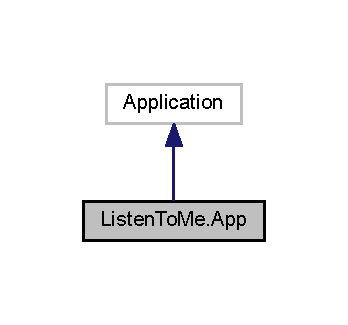
\includegraphics[width=167pt]{class_listen_to_me_1_1_app__inherit__graph}
\end{center}
\end{figure}
\subsection*{Public Member Functions}
\begin{DoxyCompactItemize}
\item 
\mbox{\hyperlink{class_listen_to_me_1_1_app_a8b865aa5eb8e0a1333c2b29f41bf4aa1}{App}} ()
\begin{DoxyCompactList}\small\item\em the Dictionary is filled if the Debug mode is not enabled instead of sections\+List \end{DoxyCompactList}\end{DoxyCompactItemize}
\subsection*{Static Public Attributes}
\begin{DoxyCompactItemize}
\item 
static System.\+Collections.\+Hashtable \mbox{\hyperlink{class_listen_to_me_1_1_app_a311ccaa1ae0fd9cf9f89d3e3466098fe}{hash\+Table}}
\begin{DoxyCompactList}\small\item\em saves the adresses of the input fields present in the frame; this helps identifying the control in which to display the textvalue recognized by Luis \end{DoxyCompactList}\item 
static Bot \mbox{\hyperlink{class_listen_to_me_1_1_app_a2862b032c76095016dd7dc7600bfd029}{Bot}}
\begin{DoxyCompactList}\small\item\em connects via Direct\+Line tho the Web\+App. Communicates with the language understanding intelligence model \end{DoxyCompactList}\item 
static Service1\+Client \mbox{\hyperlink{class_listen_to_me_1_1_app_a41b762ac78fada5d35954d39419b8e36}{client}}
\begin{DoxyCompactList}\small\item\em the W\+C\+F-\/\+Service client instance that is able to parse the H\+T\+M\+L-\/\+Form \end{DoxyCompactList}\item 
static \mbox{\hyperlink{class_listen_to_me_1_1_model_1_1_form}{Model.\+Form}} \mbox{\hyperlink{class_listen_to_me_1_1_app_a3e094e220103fe4590cf50c22f38ee65}{formstore}} = new \mbox{\hyperlink{class_listen_to_me_1_1_model_1_1_form}{Model.\+Form}}()
\begin{DoxyCompactList}\small\item\em keeps a collection Model.\+Form\+Store.\+Sections of all the sections of the web form. is able to store and load sections in the device storage \end{DoxyCompactList}\end{DoxyCompactItemize}
\subsection*{Protected Member Functions}
\begin{DoxyCompactItemize}
\item 
override void \mbox{\hyperlink{class_listen_to_me_1_1_app_ace89a3624e2de8cc528dea8b1288d03f}{On\+Launched}} (Launch\+Activated\+Event\+Args e)
\begin{DoxyCompactList}\small\item\em Is called as the application is started normally by the user. Other enty points are used for example if the application is activated in the fore or background \end{DoxyCompactList}\item 
async override void \mbox{\hyperlink{class_listen_to_me_1_1_app_a3e2da49bb555b7fdc5858f5442d396e4}{On\+Activated}} (I\+Activated\+Event\+Args e)
\begin{DoxyCompactList}\small\item\em is called whenever an external application e.\+g-\/ Cortana launches the Listen\+To\+Me\+App \end{DoxyCompactList}\end{DoxyCompactItemize}
\subsection*{Properties}
\begin{DoxyCompactItemize}
\item 
static Navigation\+Service \mbox{\hyperlink{class_listen_to_me_1_1_app_ae35ddc10bf8aad1a80c92c71c6e3b7fc}{Navigation\+Service}}\hspace{0.3cm}{\ttfamily  \mbox{[}get, private set\mbox{]}}
\begin{DoxyCompactList}\small\item\em Navigation service, provides a decoupled way to trigger the UI Frame to transition between views. \end{DoxyCompactList}\item 
static Password\+Vault \mbox{\hyperlink{class_listen_to_me_1_1_app_ad1b3a77f44f52055446727716abfccc6}{Vault}}\hspace{0.3cm}{\ttfamily  \mbox{[}get, set\mbox{]}}
\begin{DoxyCompactList}\small\item\em The password vault stores application specific usernames and passwords encrypted \end{DoxyCompactList}\end{DoxyCompactItemize}
\subsection*{Private Member Functions}
\begin{DoxyCompactItemize}
\item 
async void \mbox{\hyperlink{class_listen_to_me_1_1_app_ac79758b58c56c49b87a3e2ff6a9ad638}{Activate\+Voice\+Commands}} ()
\begin{DoxyCompactList}\small\item\em The method Activate\+Voice\+Commands is calling an Voice\+Commands.\+xml-\/\+File from local storage to determine which Cortana commands are valid. It also is able to update the phrase lists page and sections. The problem with that is, though that the phrase lists are limited to one word.\+7 For a voice command like \char`\"{}\+Open \textquotesingle{}\+Angaben zum antragsstellenden Unternehmen\textquotesingle{}\char`\"{} this is problematic. \end{DoxyCompactList}\item 
void \mbox{\hyperlink{class_listen_to_me_1_1_app_a4a8894ffc0736b646470c2a8ad6fca0d}{Init\+Gui}} (Launch\+Activated\+Event\+Args e=null)
\begin{DoxyCompactList}\small\item\em init\+Gui determines whether or not there is an active Windows Frame. It creates one for the application if there wasn\textquotesingle{}t one before. As soon as there exists a frame, the method can transfer launch\+Arguments to it. This is curently not used but might be in the future interesting. The command Edit could by this concept get the launch argument \char`\"{}company details\char`\"{} and is navigating the frame to companydails page. \end{DoxyCompactList}\item 
async Task \mbox{\hyperlink{class_listen_to_me_1_1_app_aaf710baa7ee4fb8e6da7e97a333e6e8c}{Perform\+Command\+Async}} (string command\+Name, String result)
\begin{DoxyCompactList}\small\item\em perform\+Command performs the voice commmand it received from Cortana or the input text field. \end{DoxyCompactList}\item 
void \mbox{\hyperlink{class_listen_to_me_1_1_app_a8867647372e101bdd100a68eab4d0d3a}{On\+Navigation\+Failed}} (object sender, Navigation\+Failed\+Event\+Args e)
\begin{DoxyCompactList}\small\item\em Is called when nvigation to a certain page fails \end{DoxyCompactList}\item 
void \mbox{\hyperlink{class_listen_to_me_1_1_app_adc9d18402a7a696ca6d4a7631a610e8d}{On\+Suspending}} (object sender, Suspending\+Event\+Args e)
\begin{DoxyCompactList}\small\item\em On\+Suspending is called if the application execution is stopped. The application state is stored without knowing whether the application is terminated or will be called at a later time \end{DoxyCompactList}\end{DoxyCompactItemize}
\subsection*{Private Attributes}
\begin{DoxyCompactItemize}
\item 
Root\+Frame\+Navigation\+Helper \mbox{\hyperlink{class_listen_to_me_1_1_app_a92eb573f880ce92d5b9fa79b90ba3f41}{root\+Frame\+Navigation\+Helper}}
\begin{DoxyCompactList}\small\item\em The rootframenavigation helper instance enables \mbox{\hyperlink{class_listen_to_me_1_1_app}{App}} to register to keayboard events related to navigation \end{DoxyCompactList}\end{DoxyCompactItemize}


\subsection{Detailed Description}
contains application specific methods for starting the application. Initializations and state-\/related actions are includes. 



\subsection{Constructor \& Destructor Documentation}
\mbox{\Hypertarget{class_listen_to_me_1_1_app_a8b865aa5eb8e0a1333c2b29f41bf4aa1}\label{class_listen_to_me_1_1_app_a8b865aa5eb8e0a1333c2b29f41bf4aa1}} 
\index{Listen\+To\+Me\+::\+App@{Listen\+To\+Me\+::\+App}!App@{App}}
\index{App@{App}!Listen\+To\+Me\+::\+App@{Listen\+To\+Me\+::\+App}}
\subsubsection{\texorpdfstring{App()}{App()}}
{\footnotesize\ttfamily Listen\+To\+Me.\+App.\+App (\begin{DoxyParamCaption}{ }\end{DoxyParamCaption})}



the Dictionary is filled if the Debug mode is not enabled instead of sections\+List 

Initialized the Singleton application object. This is the first line of built code and the logic equivalent to main() that is Win\+Main(). the Max\+Received\+Buffer\+Size is important because Get\+All\+Elements() returns a message 2$^\wedge$16$\ast$100 and 2$^\wedge$16 is the max default value reference \href{https://stackoverflow.com/questions/16173835/wcf-error-the-server-did-not-provide-a-meaningful-reply}{\tt https\+://stackoverflow.\+com/questions/16173835/wcf-\/error-\/the-\/server-\/did-\/not-\/provide-\/a-\/meaningful-\/reply}

\subsection{Member Function Documentation}
\mbox{\Hypertarget{class_listen_to_me_1_1_app_ac79758b58c56c49b87a3e2ff6a9ad638}\label{class_listen_to_me_1_1_app_ac79758b58c56c49b87a3e2ff6a9ad638}} 
\index{Listen\+To\+Me\+::\+App@{Listen\+To\+Me\+::\+App}!Activate\+Voice\+Commands@{Activate\+Voice\+Commands}}
\index{Activate\+Voice\+Commands@{Activate\+Voice\+Commands}!Listen\+To\+Me\+::\+App@{Listen\+To\+Me\+::\+App}}
\subsubsection{\texorpdfstring{Activate\+Voice\+Commands()}{ActivateVoiceCommands()}}
{\footnotesize\ttfamily async void Listen\+To\+Me.\+App.\+Activate\+Voice\+Commands (\begin{DoxyParamCaption}{ }\end{DoxyParamCaption})\hspace{0.3cm}{\ttfamily [private]}}



The method Activate\+Voice\+Commands is calling an Voice\+Commands.\+xml-\/\+File from local storage to determine which Cortana commands are valid. It also is able to update the phrase lists page and sections. The problem with that is, though that the phrase lists are limited to one word.\+7 For a voice command like \char`\"{}\+Open \textquotesingle{}\+Angaben zum antragsstellenden Unternehmen\textquotesingle{}\char`\"{} this is problematic. 

\mbox{\Hypertarget{class_listen_to_me_1_1_app_a4a8894ffc0736b646470c2a8ad6fca0d}\label{class_listen_to_me_1_1_app_a4a8894ffc0736b646470c2a8ad6fca0d}} 
\index{Listen\+To\+Me\+::\+App@{Listen\+To\+Me\+::\+App}!Init\+Gui@{Init\+Gui}}
\index{Init\+Gui@{Init\+Gui}!Listen\+To\+Me\+::\+App@{Listen\+To\+Me\+::\+App}}
\subsubsection{\texorpdfstring{Init\+Gui()}{InitGui()}}
{\footnotesize\ttfamily void Listen\+To\+Me.\+App.\+Init\+Gui (\begin{DoxyParamCaption}\item[{Launch\+Activated\+Event\+Args}]{e = {\ttfamily null} }\end{DoxyParamCaption})\hspace{0.3cm}{\ttfamily [private]}}



init\+Gui determines whether or not there is an active Windows Frame. It creates one for the application if there wasn\textquotesingle{}t one before. As soon as there exists a frame, the method can transfer launch\+Arguments to it. This is curently not used but might be in the future interesting. The command Edit could by this concept get the launch argument \char`\"{}company details\char`\"{} and is navigating the frame to companydails page. 


\begin{DoxyParams}{Parameters}
{\em e} & \\
\hline
\end{DoxyParams}
\mbox{\Hypertarget{class_listen_to_me_1_1_app_a3e2da49bb555b7fdc5858f5442d396e4}\label{class_listen_to_me_1_1_app_a3e2da49bb555b7fdc5858f5442d396e4}} 
\index{Listen\+To\+Me\+::\+App@{Listen\+To\+Me\+::\+App}!On\+Activated@{On\+Activated}}
\index{On\+Activated@{On\+Activated}!Listen\+To\+Me\+::\+App@{Listen\+To\+Me\+::\+App}}
\subsubsection{\texorpdfstring{On\+Activated()}{OnActivated()}}
{\footnotesize\ttfamily async override void Listen\+To\+Me.\+App.\+On\+Activated (\begin{DoxyParamCaption}\item[{I\+Activated\+Event\+Args}]{e }\end{DoxyParamCaption})\hspace{0.3cm}{\ttfamily [protected]}}



is called whenever an external application e.\+g-\/ Cortana launches the Listen\+To\+Me\+App 

\mbox{\Hypertarget{class_listen_to_me_1_1_app_ace89a3624e2de8cc528dea8b1288d03f}\label{class_listen_to_me_1_1_app_ace89a3624e2de8cc528dea8b1288d03f}} 
\index{Listen\+To\+Me\+::\+App@{Listen\+To\+Me\+::\+App}!On\+Launched@{On\+Launched}}
\index{On\+Launched@{On\+Launched}!Listen\+To\+Me\+::\+App@{Listen\+To\+Me\+::\+App}}
\subsubsection{\texorpdfstring{On\+Launched()}{OnLaunched()}}
{\footnotesize\ttfamily override void Listen\+To\+Me.\+App.\+On\+Launched (\begin{DoxyParamCaption}\item[{Launch\+Activated\+Event\+Args}]{e }\end{DoxyParamCaption})\hspace{0.3cm}{\ttfamily [protected]}}



Is called as the application is started normally by the user. Other enty points are used for example if the application is activated in the fore or background 


\begin{DoxyParams}{Parameters}
{\em e} & Details on application start and start arguments.\\
\hline
\end{DoxyParams}
\mbox{\Hypertarget{class_listen_to_me_1_1_app_a8867647372e101bdd100a68eab4d0d3a}\label{class_listen_to_me_1_1_app_a8867647372e101bdd100a68eab4d0d3a}} 
\index{Listen\+To\+Me\+::\+App@{Listen\+To\+Me\+::\+App}!On\+Navigation\+Failed@{On\+Navigation\+Failed}}
\index{On\+Navigation\+Failed@{On\+Navigation\+Failed}!Listen\+To\+Me\+::\+App@{Listen\+To\+Me\+::\+App}}
\subsubsection{\texorpdfstring{On\+Navigation\+Failed()}{OnNavigationFailed()}}
{\footnotesize\ttfamily void Listen\+To\+Me.\+App.\+On\+Navigation\+Failed (\begin{DoxyParamCaption}\item[{object}]{sender,  }\item[{Navigation\+Failed\+Event\+Args}]{e }\end{DoxyParamCaption})\hspace{0.3cm}{\ttfamily [private]}}



Is called when nvigation to a certain page fails 


\begin{DoxyParams}{Parameters}
{\em sender} & Frame that failed to navigate to the page\\
\hline
{\em e} & Details about navigation error\\
\hline
\end{DoxyParams}
\mbox{\Hypertarget{class_listen_to_me_1_1_app_adc9d18402a7a696ca6d4a7631a610e8d}\label{class_listen_to_me_1_1_app_adc9d18402a7a696ca6d4a7631a610e8d}} 
\index{Listen\+To\+Me\+::\+App@{Listen\+To\+Me\+::\+App}!On\+Suspending@{On\+Suspending}}
\index{On\+Suspending@{On\+Suspending}!Listen\+To\+Me\+::\+App@{Listen\+To\+Me\+::\+App}}
\subsubsection{\texorpdfstring{On\+Suspending()}{OnSuspending()}}
{\footnotesize\ttfamily void Listen\+To\+Me.\+App.\+On\+Suspending (\begin{DoxyParamCaption}\item[{object}]{sender,  }\item[{Suspending\+Event\+Args}]{e }\end{DoxyParamCaption})\hspace{0.3cm}{\ttfamily [private]}}



On\+Suspending is called if the application execution is stopped. The application state is stored without knowing whether the application is terminated or will be called at a later time 


\begin{DoxyParams}{Parameters}
{\em sender} & Source of suspension.\\
\hline
{\em e} & Details on suspension.\\
\hline
\end{DoxyParams}
\mbox{\Hypertarget{class_listen_to_me_1_1_app_aaf710baa7ee4fb8e6da7e97a333e6e8c}\label{class_listen_to_me_1_1_app_aaf710baa7ee4fb8e6da7e97a333e6e8c}} 
\index{Listen\+To\+Me\+::\+App@{Listen\+To\+Me\+::\+App}!Perform\+Command\+Async@{Perform\+Command\+Async}}
\index{Perform\+Command\+Async@{Perform\+Command\+Async}!Listen\+To\+Me\+::\+App@{Listen\+To\+Me\+::\+App}}
\subsubsection{\texorpdfstring{Perform\+Command\+Async()}{PerformCommandAsync()}}
{\footnotesize\ttfamily async Task Listen\+To\+Me.\+App.\+Perform\+Command\+Async (\begin{DoxyParamCaption}\item[{string}]{command\+Name,  }\item[{String}]{result }\end{DoxyParamCaption})\hspace{0.3cm}{\ttfamily [private]}}



perform\+Command performs the voice commmand it received from Cortana or the input text field. 


\begin{DoxyParams}{Parameters}
{\em command\+Name} & The name ot the command, e.\+g. edit. Valid names are found in Vice\+Connamds.\+xml\\
\hline
{\em result} & The speech recognition result in text form\\
\hline
\end{DoxyParams}
\begin{DoxyReturn}{Returns}

\end{DoxyReturn}


\subsection{Member Data Documentation}
\mbox{\Hypertarget{class_listen_to_me_1_1_app_a2862b032c76095016dd7dc7600bfd029}\label{class_listen_to_me_1_1_app_a2862b032c76095016dd7dc7600bfd029}} 
\index{Listen\+To\+Me\+::\+App@{Listen\+To\+Me\+::\+App}!Bot@{Bot}}
\index{Bot@{Bot}!Listen\+To\+Me\+::\+App@{Listen\+To\+Me\+::\+App}}
\subsubsection{\texorpdfstring{Bot}{Bot}}
{\footnotesize\ttfamily Bot Listen\+To\+Me.\+App.\+Bot\hspace{0.3cm}{\ttfamily [static]}}



connects via Direct\+Line tho the Web\+App. Communicates with the language understanding intelligence model 

\mbox{\Hypertarget{class_listen_to_me_1_1_app_a41b762ac78fada5d35954d39419b8e36}\label{class_listen_to_me_1_1_app_a41b762ac78fada5d35954d39419b8e36}} 
\index{Listen\+To\+Me\+::\+App@{Listen\+To\+Me\+::\+App}!client@{client}}
\index{client@{client}!Listen\+To\+Me\+::\+App@{Listen\+To\+Me\+::\+App}}
\subsubsection{\texorpdfstring{client}{client}}
{\footnotesize\ttfamily Service1\+Client Listen\+To\+Me.\+App.\+client\hspace{0.3cm}{\ttfamily [static]}}



the W\+C\+F-\/\+Service client instance that is able to parse the H\+T\+M\+L-\/\+Form 

\mbox{\Hypertarget{class_listen_to_me_1_1_app_a3e094e220103fe4590cf50c22f38ee65}\label{class_listen_to_me_1_1_app_a3e094e220103fe4590cf50c22f38ee65}} 
\index{Listen\+To\+Me\+::\+App@{Listen\+To\+Me\+::\+App}!formstore@{formstore}}
\index{formstore@{formstore}!Listen\+To\+Me\+::\+App@{Listen\+To\+Me\+::\+App}}
\subsubsection{\texorpdfstring{formstore}{formstore}}
{\footnotesize\ttfamily \mbox{\hyperlink{class_listen_to_me_1_1_model_1_1_form}{Model.\+Form}} Listen\+To\+Me.\+App.\+formstore = new \mbox{\hyperlink{class_listen_to_me_1_1_model_1_1_form}{Model.\+Form}}()\hspace{0.3cm}{\ttfamily [static]}}



keeps a collection Model.\+Form\+Store.\+Sections of all the sections of the web form. is able to store and load sections in the device storage 

\mbox{\Hypertarget{class_listen_to_me_1_1_app_a311ccaa1ae0fd9cf9f89d3e3466098fe}\label{class_listen_to_me_1_1_app_a311ccaa1ae0fd9cf9f89d3e3466098fe}} 
\index{Listen\+To\+Me\+::\+App@{Listen\+To\+Me\+::\+App}!hash\+Table@{hash\+Table}}
\index{hash\+Table@{hash\+Table}!Listen\+To\+Me\+::\+App@{Listen\+To\+Me\+::\+App}}
\subsubsection{\texorpdfstring{hash\+Table}{hashTable}}
{\footnotesize\ttfamily System.\+Collections.\+Hashtable Listen\+To\+Me.\+App.\+hash\+Table\hspace{0.3cm}{\ttfamily [static]}}



saves the adresses of the input fields present in the frame; this helps identifying the control in which to display the textvalue recognized by Luis 

\mbox{\Hypertarget{class_listen_to_me_1_1_app_a92eb573f880ce92d5b9fa79b90ba3f41}\label{class_listen_to_me_1_1_app_a92eb573f880ce92d5b9fa79b90ba3f41}} 
\index{Listen\+To\+Me\+::\+App@{Listen\+To\+Me\+::\+App}!root\+Frame\+Navigation\+Helper@{root\+Frame\+Navigation\+Helper}}
\index{root\+Frame\+Navigation\+Helper@{root\+Frame\+Navigation\+Helper}!Listen\+To\+Me\+::\+App@{Listen\+To\+Me\+::\+App}}
\subsubsection{\texorpdfstring{root\+Frame\+Navigation\+Helper}{rootFrameNavigationHelper}}
{\footnotesize\ttfamily Root\+Frame\+Navigation\+Helper Listen\+To\+Me.\+App.\+root\+Frame\+Navigation\+Helper\hspace{0.3cm}{\ttfamily [private]}}



The rootframenavigation helper instance enables \mbox{\hyperlink{class_listen_to_me_1_1_app}{App}} to register to keayboard events related to navigation 



\subsection{Property Documentation}
\mbox{\Hypertarget{class_listen_to_me_1_1_app_ae35ddc10bf8aad1a80c92c71c6e3b7fc}\label{class_listen_to_me_1_1_app_ae35ddc10bf8aad1a80c92c71c6e3b7fc}} 
\index{Listen\+To\+Me\+::\+App@{Listen\+To\+Me\+::\+App}!Navigation\+Service@{Navigation\+Service}}
\index{Navigation\+Service@{Navigation\+Service}!Listen\+To\+Me\+::\+App@{Listen\+To\+Me\+::\+App}}
\subsubsection{\texorpdfstring{Navigation\+Service}{NavigationService}}
{\footnotesize\ttfamily Navigation\+Service Listen\+To\+Me.\+App.\+Navigation\+Service\hspace{0.3cm}{\ttfamily [static]}, {\ttfamily [get]}, {\ttfamily [private set]}}



Navigation service, provides a decoupled way to trigger the UI Frame to transition between views. 

\mbox{\Hypertarget{class_listen_to_me_1_1_app_ad1b3a77f44f52055446727716abfccc6}\label{class_listen_to_me_1_1_app_ad1b3a77f44f52055446727716abfccc6}} 
\index{Listen\+To\+Me\+::\+App@{Listen\+To\+Me\+::\+App}!Vault@{Vault}}
\index{Vault@{Vault}!Listen\+To\+Me\+::\+App@{Listen\+To\+Me\+::\+App}}
\subsubsection{\texorpdfstring{Vault}{Vault}}
{\footnotesize\ttfamily Password\+Vault Listen\+To\+Me.\+App.\+Vault\hspace{0.3cm}{\ttfamily [static]}, {\ttfamily [get]}, {\ttfamily [set]}}



The password vault stores application specific usernames and passwords encrypted 



The documentation for this class was generated from the following file\+:\begin{DoxyCompactItemize}
\item 
C\+:/\+Users/fgeissle/source/repos/\+F\+B\+K\+Voice\+App/\+Listen\+To\+Me/\mbox{\hyperlink{_app_8xaml_8cs}{App.\+xaml.\+cs}}\end{DoxyCompactItemize}

\hypertarget{class_listen_to_me_1_1_cortana_model_methods}{}\section{Listen\+To\+Me.\+Cortana\+Model\+Methods Class Reference}
\label{class_listen_to_me_1_1_cortana_model_methods}\index{Listen\+To\+Me.\+Cortana\+Model\+Methods@{Listen\+To\+Me.\+Cortana\+Model\+Methods}}


Contains methods that update the cortana voice command definition file to make it more dynamic. Note\+: This doesn\textquotesingle{}t work as intendet, because phrase lists are only allowing one word entries and the form headings are mostly more than one word long.  




Inheritance diagram for Listen\+To\+Me.\+Cortana\+Model\+Methods\+:\nopagebreak
\begin{figure}[H]
\begin{center}
\leavevmode
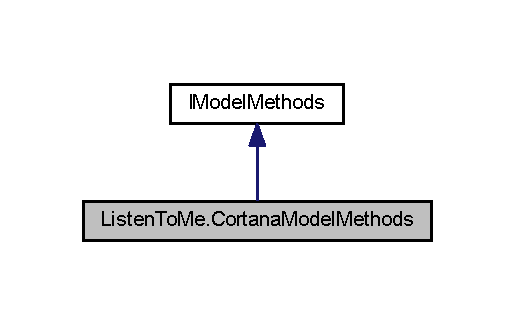
\includegraphics[width=247pt]{class_listen_to_me_1_1_cortana_model_methods__inherit__graph}
\end{center}
\end{figure}
\subsection*{Public Member Functions}
\begin{DoxyCompactItemize}
\item 
async Task$<$ List$<$ String $>$ $>$ \mbox{\hyperlink{class_listen_to_me_1_1_cortana_model_methods_afe872337c3f1c74f5db6e26918f29ac1}{Update\+Phrase\+List}} (String phraselist\+Name)
\begin{DoxyCompactList}\small\item\em reference Trip\+View\+Model.\+Update\+Destination\+Phrase\+List in Adventure\+Works project called when \mbox{\hyperlink{class_listen_to_me_1_1_app}{App}} Activates Voice\+Commands, this method fills the collections of tags from the html Form and updates the Voice\+Command-\/xml File \end{DoxyCompactList}\end{DoxyCompactItemize}


\subsection{Detailed Description}
Contains methods that update the cortana voice command definition file to make it more dynamic. Note\+: This doesn\textquotesingle{}t work as intendet, because phrase lists are only allowing one word entries and the form headings are mostly more than one word long. 



\subsection{Member Function Documentation}
\mbox{\Hypertarget{class_listen_to_me_1_1_cortana_model_methods_afe872337c3f1c74f5db6e26918f29ac1}\label{class_listen_to_me_1_1_cortana_model_methods_afe872337c3f1c74f5db6e26918f29ac1}} 
\index{Listen\+To\+Me\+::\+Cortana\+Model\+Methods@{Listen\+To\+Me\+::\+Cortana\+Model\+Methods}!Update\+Phrase\+List@{Update\+Phrase\+List}}
\index{Update\+Phrase\+List@{Update\+Phrase\+List}!Listen\+To\+Me\+::\+Cortana\+Model\+Methods@{Listen\+To\+Me\+::\+Cortana\+Model\+Methods}}
\subsubsection{\texorpdfstring{Update\+Phrase\+List()}{UpdatePhraseList()}}
{\footnotesize\ttfamily async Task$<$List$<$String$>$ $>$ Listen\+To\+Me.\+Cortana\+Model\+Methods.\+Update\+Phrase\+List (\begin{DoxyParamCaption}\item[{String}]{phraselist\+Name }\end{DoxyParamCaption})}



reference Trip\+View\+Model.\+Update\+Destination\+Phrase\+List in Adventure\+Works project called when \mbox{\hyperlink{class_listen_to_me_1_1_app}{App}} Activates Voice\+Commands, this method fills the collections of tags from the html Form and updates the Voice\+Command-\/xml File 



The documentation for this class was generated from the following file\+:\begin{DoxyCompactItemize}
\item 
C\+:/\+Users/fgeissle/source/repos/\+F\+B\+K\+Voice\+App/\+Listen\+To\+Me/\mbox{\hyperlink{_cortana_model_methods_8cs}{Cortana\+Model\+Methods.\+cs}}\end{DoxyCompactItemize}

\hypertarget{class_listen_to_me_1_1_dynamic_page}{}\section{Listen\+To\+Me.\+Dynamic\+Page Class Reference}
\label{class_listen_to_me_1_1_dynamic_page}\index{Listen\+To\+Me.\+Dynamic\+Page@{Listen\+To\+Me.\+Dynamic\+Page}}


This is a page that can be dynamically filled in \mbox{\hyperlink{class_listen_to_me_1_1_main_page}{Main\+Page}}. It is used to display the components that the wcf service finds per section on the form  




Inheritance diagram for Listen\+To\+Me.\+Dynamic\+Page\+:\nopagebreak
\begin{figure}[H]
\begin{center}
\leavevmode
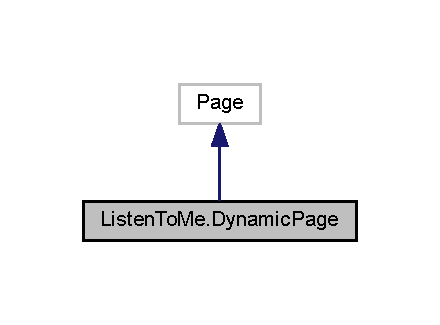
\includegraphics[width=211pt]{class_listen_to_me_1_1_dynamic_page__inherit__graph}
\end{center}
\end{figure}
\subsection*{Public Member Functions}
\begin{DoxyCompactItemize}
\item 
\mbox{\hyperlink{class_listen_to_me_1_1_dynamic_page_aee4e65517f3b3f4bda37fec075ee0371}{Dynamic\+Page}} ()
\end{DoxyCompactItemize}
\subsection*{Protected Member Functions}
\begin{DoxyCompactItemize}
\item 
override void \mbox{\hyperlink{class_listen_to_me_1_1_dynamic_page_abe7cf843906f8a930d2bdd2ade17ea0b}{On\+Navigated\+To}} (Navigation\+Event\+Args e)
\begin{DoxyCompactList}\small\item\em On\+Navigated\+To fills the Dynamic\+Pages\textquotesingle{}s Grid element with a stackpanel that contains all fields of a section \end{DoxyCompactList}\item 
override void \mbox{\hyperlink{class_listen_to_me_1_1_dynamic_page_a042e3936e2668147cd280d2428ef793b}{On\+Navigated\+From}} (Navigation\+Event\+Args e)
\begin{DoxyCompactList}\small\item\em called when the page is unloaded. Since there is navigation whenever the \textquotesingle{}next\textquotesingle{} button is hit the Layout grid has to be deleted. \end{DoxyCompactList}\end{DoxyCompactItemize}
\subsection*{Properties}
\begin{DoxyCompactItemize}
\item 
Stack\+Panel \mbox{\hyperlink{class_listen_to_me_1_1_dynamic_page_a187c4aba2636c3956cf023f1dc3f86ec}{my\+Panel}}\hspace{0.3cm}{\ttfamily  \mbox{[}get, set\mbox{]}}
\end{DoxyCompactItemize}
\subsection*{Private Member Functions}
\begin{DoxyCompactItemize}
\item 
void \mbox{\hyperlink{class_listen_to_me_1_1_dynamic_page_ab3716b91cf48530310b3cd6ce47506a3}{save\+Section}} (int index)
\end{DoxyCompactItemize}


\subsection{Detailed Description}
This is a page that can be dynamically filled in \mbox{\hyperlink{class_listen_to_me_1_1_main_page}{Main\+Page}}. It is used to display the components that the wcf service finds per section on the form 



\subsection{Constructor \& Destructor Documentation}
\mbox{\Hypertarget{class_listen_to_me_1_1_dynamic_page_aee4e65517f3b3f4bda37fec075ee0371}\label{class_listen_to_me_1_1_dynamic_page_aee4e65517f3b3f4bda37fec075ee0371}} 
\index{Listen\+To\+Me\+::\+Dynamic\+Page@{Listen\+To\+Me\+::\+Dynamic\+Page}!Dynamic\+Page@{Dynamic\+Page}}
\index{Dynamic\+Page@{Dynamic\+Page}!Listen\+To\+Me\+::\+Dynamic\+Page@{Listen\+To\+Me\+::\+Dynamic\+Page}}
\subsubsection{\texorpdfstring{Dynamic\+Page()}{DynamicPage()}}
{\footnotesize\ttfamily Listen\+To\+Me.\+Dynamic\+Page.\+Dynamic\+Page (\begin{DoxyParamCaption}{ }\end{DoxyParamCaption})}



\subsection{Member Function Documentation}
\mbox{\Hypertarget{class_listen_to_me_1_1_dynamic_page_a042e3936e2668147cd280d2428ef793b}\label{class_listen_to_me_1_1_dynamic_page_a042e3936e2668147cd280d2428ef793b}} 
\index{Listen\+To\+Me\+::\+Dynamic\+Page@{Listen\+To\+Me\+::\+Dynamic\+Page}!On\+Navigated\+From@{On\+Navigated\+From}}
\index{On\+Navigated\+From@{On\+Navigated\+From}!Listen\+To\+Me\+::\+Dynamic\+Page@{Listen\+To\+Me\+::\+Dynamic\+Page}}
\subsubsection{\texorpdfstring{On\+Navigated\+From()}{OnNavigatedFrom()}}
{\footnotesize\ttfamily override void Listen\+To\+Me.\+Dynamic\+Page.\+On\+Navigated\+From (\begin{DoxyParamCaption}\item[{Navigation\+Event\+Args}]{e }\end{DoxyParamCaption})\hspace{0.3cm}{\ttfamily [protected]}}



called when the page is unloaded. Since there is navigation whenever the \textquotesingle{}next\textquotesingle{} button is hit the Layout grid has to be deleted. 


\begin{DoxyParams}{Parameters}
{\em e} & \\
\hline
\end{DoxyParams}
\mbox{\Hypertarget{class_listen_to_me_1_1_dynamic_page_abe7cf843906f8a930d2bdd2ade17ea0b}\label{class_listen_to_me_1_1_dynamic_page_abe7cf843906f8a930d2bdd2ade17ea0b}} 
\index{Listen\+To\+Me\+::\+Dynamic\+Page@{Listen\+To\+Me\+::\+Dynamic\+Page}!On\+Navigated\+To@{On\+Navigated\+To}}
\index{On\+Navigated\+To@{On\+Navigated\+To}!Listen\+To\+Me\+::\+Dynamic\+Page@{Listen\+To\+Me\+::\+Dynamic\+Page}}
\subsubsection{\texorpdfstring{On\+Navigated\+To()}{OnNavigatedTo()}}
{\footnotesize\ttfamily override void Listen\+To\+Me.\+Dynamic\+Page.\+On\+Navigated\+To (\begin{DoxyParamCaption}\item[{Navigation\+Event\+Args}]{e }\end{DoxyParamCaption})\hspace{0.3cm}{\ttfamily [protected]}}



On\+Navigated\+To fills the Dynamic\+Pages\textquotesingle{}s Grid element with a stackpanel that contains all fields of a section 


\begin{DoxyParams}{Parameters}
{\em e} & the stackpanel provided by Navigation\+Service.\+Navigate(\+Dynamic\+Page, stackpanel)-\/method\\
\hline
\end{DoxyParams}
\mbox{\Hypertarget{class_listen_to_me_1_1_dynamic_page_ab3716b91cf48530310b3cd6ce47506a3}\label{class_listen_to_me_1_1_dynamic_page_ab3716b91cf48530310b3cd6ce47506a3}} 
\index{Listen\+To\+Me\+::\+Dynamic\+Page@{Listen\+To\+Me\+::\+Dynamic\+Page}!save\+Section@{save\+Section}}
\index{save\+Section@{save\+Section}!Listen\+To\+Me\+::\+Dynamic\+Page@{Listen\+To\+Me\+::\+Dynamic\+Page}}
\subsubsection{\texorpdfstring{save\+Section()}{saveSection()}}
{\footnotesize\ttfamily void Listen\+To\+Me.\+Dynamic\+Page.\+save\+Section (\begin{DoxyParamCaption}\item[{int}]{index }\end{DoxyParamCaption})\hspace{0.3cm}{\ttfamily [private]}}



\subsection{Property Documentation}
\mbox{\Hypertarget{class_listen_to_me_1_1_dynamic_page_a187c4aba2636c3956cf023f1dc3f86ec}\label{class_listen_to_me_1_1_dynamic_page_a187c4aba2636c3956cf023f1dc3f86ec}} 
\index{Listen\+To\+Me\+::\+Dynamic\+Page@{Listen\+To\+Me\+::\+Dynamic\+Page}!my\+Panel@{my\+Panel}}
\index{my\+Panel@{my\+Panel}!Listen\+To\+Me\+::\+Dynamic\+Page@{Listen\+To\+Me\+::\+Dynamic\+Page}}
\subsubsection{\texorpdfstring{my\+Panel}{myPanel}}
{\footnotesize\ttfamily Stack\+Panel Listen\+To\+Me.\+Dynamic\+Page.\+my\+Panel\hspace{0.3cm}{\ttfamily [get]}, {\ttfamily [set]}, {\ttfamily [private]}}



The documentation for this class was generated from the following file\+:\begin{DoxyCompactItemize}
\item 
C\+:/\+Users/fgeissle/source/repos/\+F\+B\+K\+Voice\+App/\+Listen\+To\+Me/\mbox{\hyperlink{_dynamic_page_8xaml_8cs}{Dynamic\+Page.\+xaml.\+cs}}\end{DoxyCompactItemize}

\hypertarget{class_listen_to_me_1_1_model_1_1_entity}{}\section{Listen\+To\+Me.\+Model.\+Entity Class Reference}
\label{class_listen_to_me_1_1_model_1_1_entity}\index{Listen\+To\+Me.\+Model.\+Entity@{Listen\+To\+Me.\+Model.\+Entity}}


subclass of Root\+Object. Note\+: these classes were easily pasted in C\# using the visual studio tools for converting J\+S\+ON  


\subsection*{Properties}
\begin{DoxyCompactItemize}
\item 
string {\bfseries entity}\hspace{0.3cm}{\ttfamily  \mbox{[}get, set\mbox{]}}\hypertarget{class_listen_to_me_1_1_model_1_1_entity_a4ae17435557f0e0ec97ff0a93f791f63}{}\label{class_listen_to_me_1_1_model_1_1_entity_a4ae17435557f0e0ec97ff0a93f791f63}

\item 
string {\bfseries type}\hspace{0.3cm}{\ttfamily  \mbox{[}get, set\mbox{]}}\hypertarget{class_listen_to_me_1_1_model_1_1_entity_af2daeab3bb0f1ec71b0664aad418ac65}{}\label{class_listen_to_me_1_1_model_1_1_entity_af2daeab3bb0f1ec71b0664aad418ac65}

\item 
int {\bfseries start\+Index}\hspace{0.3cm}{\ttfamily  \mbox{[}get, set\mbox{]}}\hypertarget{class_listen_to_me_1_1_model_1_1_entity_a32c85bf1ead96ed642a8164fb425c274}{}\label{class_listen_to_me_1_1_model_1_1_entity_a32c85bf1ead96ed642a8164fb425c274}

\item 
int {\bfseries end\+Index}\hspace{0.3cm}{\ttfamily  \mbox{[}get, set\mbox{]}}\hypertarget{class_listen_to_me_1_1_model_1_1_entity_ab4fe7e4a09235bbf2715a3049cba3efb}{}\label{class_listen_to_me_1_1_model_1_1_entity_ab4fe7e4a09235bbf2715a3049cba3efb}

\item 
float {\bfseries score}\hspace{0.3cm}{\ttfamily  \mbox{[}get, set\mbox{]}}\hypertarget{class_listen_to_me_1_1_model_1_1_entity_aed4873738d141be126a637073cae179a}{}\label{class_listen_to_me_1_1_model_1_1_entity_aed4873738d141be126a637073cae179a}

\end{DoxyCompactItemize}


\subsection{Detailed Description}
subclass of Root\+Object. Note\+: these classes were easily pasted in C\# using the visual studio tools for converting J\+S\+ON 



The documentation for this class was generated from the following file\+:\begin{DoxyCompactItemize}
\item 
C\+:/\+Users/user/source/repos/\+Hoermirzu/\+Listen\+To\+Me-\/master-\/89f0b49594deaade7bfad24dad062ff16eca36da/\+Listen\+To\+Me/\+Model/Proxy.\+cs\end{DoxyCompactItemize}

\hypertarget{class_listen_to_me_1_1_model_1_1_form}{}\section{Listen\+To\+Me.\+Model.\+Form Class Reference}
\label{class_listen_to_me_1_1_model_1_1_form}\index{Listen\+To\+Me.\+Model.\+Form@{Listen\+To\+Me.\+Model.\+Form}}


able to store Sections of the form. $<$reference$>$Adventure\+Works in U\+WP sample projects at github$<$/reference$>$ /summary$>$  


\subsection*{Public Member Functions}
\begin{DoxyCompactItemize}
\item 
\mbox{\hyperlink{class_listen_to_me_1_1_model_1_1_form_ae0301066625a452b488a25365cf369d0}{Form}} ()
\item 
async Task \mbox{\hyperlink{class_listen_to_me_1_1_model_1_1_form_a97e6f2c705e11c7c99b8742d846d8738}{Fill\+\_\+sections}} ()
\begin{DoxyCompactList}\small\item\em calls the wcf service to dertermine the structure of the form. Then, it separates the structure into sections and binds them to a static attibute that\textquotesingle{}s globally available in \mbox{\hyperlink{namespace_listen_to_me}{Listen\+To\+Me}} \mbox{\hyperlink{class_listen_to_me_1_1_app}{App}}. To which object it outputs depends on the debug mode. If debug is enabled, it will write to sections\+List. If not it will write to a Dictionary. \end{DoxyCompactList}\end{DoxyCompactItemize}
\subsection*{Properties}
\begin{DoxyCompactItemize}
\item 
Observable\+Collection$<$ Class\+Library.\+model.\+Section $>$ \mbox{\hyperlink{class_listen_to_me_1_1_model_1_1_form_a5ecdd2a344e3e2e6157ff3c5b6dfc2d1}{Sections}}\hspace{0.3cm}{\ttfamily  \mbox{[}get, set\mbox{]}}
\begin{DoxyCompactList}\small\item\em helps storing the sections collection. \end{DoxyCompactList}\end{DoxyCompactItemize}
\subsection*{Private Member Functions}
\begin{DoxyCompactItemize}
\item 
Element \mbox{\hyperlink{class_listen_to_me_1_1_model_1_1_form_a6a232d7bcb2cff3bd69cdb149c3dd485}{Match\+Text\+To\+Control}} (U\+I\+Element element, Element json\+Element)
\end{DoxyCompactItemize}
\subsection*{Private Attributes}
\begin{DoxyCompactItemize}
\item 
Observable\+Collection$<$ Class\+Library.\+model.\+Section $>$ \mbox{\hyperlink{class_listen_to_me_1_1_model_1_1_form_a4b5d6fd20dc2522f3ad05614958c9895}{sections}}
\begin{DoxyCompactList}\small\item\em flag to determine whether the page is loaded or not \end{DoxyCompactList}\end{DoxyCompactItemize}


\subsection{Detailed Description}
able to store Sections of the form. $<$reference$>$Adventure\+Works in U\+WP sample projects at github$<$/reference$>$ /summary$>$ 

\subsection{Constructor \& Destructor Documentation}
\mbox{\Hypertarget{class_listen_to_me_1_1_model_1_1_form_ae0301066625a452b488a25365cf369d0}\label{class_listen_to_me_1_1_model_1_1_form_ae0301066625a452b488a25365cf369d0}} 
\index{Listen\+To\+Me\+::\+Model\+::\+Form@{Listen\+To\+Me\+::\+Model\+::\+Form}!Form@{Form}}
\index{Form@{Form}!Listen\+To\+Me\+::\+Model\+::\+Form@{Listen\+To\+Me\+::\+Model\+::\+Form}}
\subsubsection{\texorpdfstring{Form()}{Form()}}
{\footnotesize\ttfamily Listen\+To\+Me.\+Model.\+Form.\+Form (\begin{DoxyParamCaption}{ }\end{DoxyParamCaption})}



\subsection{Member Function Documentation}
\mbox{\Hypertarget{class_listen_to_me_1_1_model_1_1_form_a97e6f2c705e11c7c99b8742d846d8738}\label{class_listen_to_me_1_1_model_1_1_form_a97e6f2c705e11c7c99b8742d846d8738}} 
\index{Listen\+To\+Me\+::\+Model\+::\+Form@{Listen\+To\+Me\+::\+Model\+::\+Form}!Fill\+\_\+sections@{Fill\+\_\+sections}}
\index{Fill\+\_\+sections@{Fill\+\_\+sections}!Listen\+To\+Me\+::\+Model\+::\+Form@{Listen\+To\+Me\+::\+Model\+::\+Form}}
\subsubsection{\texorpdfstring{Fill\+\_\+sections()}{Fill\_sections()}}
{\footnotesize\ttfamily async Task Listen\+To\+Me.\+Model.\+Form.\+Fill\+\_\+sections (\begin{DoxyParamCaption}{ }\end{DoxyParamCaption})}



calls the wcf service to dertermine the structure of the form. Then, it separates the structure into sections and binds them to a static attibute that\textquotesingle{}s globally available in \mbox{\hyperlink{namespace_listen_to_me}{Listen\+To\+Me}} \mbox{\hyperlink{class_listen_to_me_1_1_app}{App}}. To which object it outputs depends on the debug mode. If debug is enabled, it will write to sections\+List. If not it will write to a Dictionary. 

\mbox{\Hypertarget{class_listen_to_me_1_1_model_1_1_form_a6a232d7bcb2cff3bd69cdb149c3dd485}\label{class_listen_to_me_1_1_model_1_1_form_a6a232d7bcb2cff3bd69cdb149c3dd485}} 
\index{Listen\+To\+Me\+::\+Model\+::\+Form@{Listen\+To\+Me\+::\+Model\+::\+Form}!Match\+Text\+To\+Control@{Match\+Text\+To\+Control}}
\index{Match\+Text\+To\+Control@{Match\+Text\+To\+Control}!Listen\+To\+Me\+::\+Model\+::\+Form@{Listen\+To\+Me\+::\+Model\+::\+Form}}
\subsubsection{\texorpdfstring{Match\+Text\+To\+Control()}{MatchTextToControl()}}
{\footnotesize\ttfamily Element Listen\+To\+Me.\+Model.\+Form.\+Match\+Text\+To\+Control (\begin{DoxyParamCaption}\item[{U\+I\+Element}]{element,  }\item[{Element}]{json\+Element }\end{DoxyParamCaption})\hspace{0.3cm}{\ttfamily [private]}}



\subsection{Member Data Documentation}
\mbox{\Hypertarget{class_listen_to_me_1_1_model_1_1_form_a4b5d6fd20dc2522f3ad05614958c9895}\label{class_listen_to_me_1_1_model_1_1_form_a4b5d6fd20dc2522f3ad05614958c9895}} 
\index{Listen\+To\+Me\+::\+Model\+::\+Form@{Listen\+To\+Me\+::\+Model\+::\+Form}!sections@{sections}}
\index{sections@{sections}!Listen\+To\+Me\+::\+Model\+::\+Form@{Listen\+To\+Me\+::\+Model\+::\+Form}}
\subsubsection{\texorpdfstring{sections}{sections}}
{\footnotesize\ttfamily Observable\+Collection$<$Class\+Library.\+model.\+Section$>$ Listen\+To\+Me.\+Model.\+Form.\+sections\hspace{0.3cm}{\ttfamily [private]}}



flag to determine whether the page is loaded or not 

Persist the loaded fields in memory for use in other parts of the application. 

\subsection{Property Documentation}
\mbox{\Hypertarget{class_listen_to_me_1_1_model_1_1_form_a5ecdd2a344e3e2e6157ff3c5b6dfc2d1}\label{class_listen_to_me_1_1_model_1_1_form_a5ecdd2a344e3e2e6157ff3c5b6dfc2d1}} 
\index{Listen\+To\+Me\+::\+Model\+::\+Form@{Listen\+To\+Me\+::\+Model\+::\+Form}!Sections@{Sections}}
\index{Sections@{Sections}!Listen\+To\+Me\+::\+Model\+::\+Form@{Listen\+To\+Me\+::\+Model\+::\+Form}}
\subsubsection{\texorpdfstring{Sections}{Sections}}
{\footnotesize\ttfamily Observable\+Collection$<$Class\+Library.\+model.\+Section$>$ Listen\+To\+Me.\+Model.\+Form.\+Sections\hspace{0.3cm}{\ttfamily [get]}, {\ttfamily [set]}}



helps storing the sections collection. 



The documentation for this class was generated from the following file\+:\begin{DoxyCompactItemize}
\item 
C\+:/\+Users/fgeissle/source/repos/\+F\+B\+K\+Voice\+App/\+Listen\+To\+Me/\+Model/\mbox{\hyperlink{_form_8cs}{Form.\+cs}}\end{DoxyCompactItemize}

\hypertarget{class_listen_to_me_1_1_model_1_1_intent}{}\section{Listen\+To\+Me.\+Model.\+Intent Class Reference}
\label{class_listen_to_me_1_1_model_1_1_intent}\index{Listen\+To\+Me.\+Model.\+Intent@{Listen\+To\+Me.\+Model.\+Intent}}


subclass of Root\+Object. Note\+: these classes were easily pasted in C\# using the visual studio tools for converting J\+S\+ON  


\subsection*{Properties}
\begin{DoxyCompactItemize}
\item 
string \mbox{\hyperlink{class_listen_to_me_1_1_model_1_1_intent_a72e3844bbc2658989213e3182068c3d4}{intent}}\hspace{0.3cm}{\ttfamily  \mbox{[}get, set\mbox{]}}
\item 
float \mbox{\hyperlink{class_listen_to_me_1_1_model_1_1_intent_a82e80d6b2c310b22beacb60637a03d20}{score}}\hspace{0.3cm}{\ttfamily  \mbox{[}get, set\mbox{]}}
\end{DoxyCompactItemize}


\subsection{Detailed Description}
subclass of Root\+Object. Note\+: these classes were easily pasted in C\# using the visual studio tools for converting J\+S\+ON 



\subsection{Property Documentation}
\mbox{\Hypertarget{class_listen_to_me_1_1_model_1_1_intent_a72e3844bbc2658989213e3182068c3d4}\label{class_listen_to_me_1_1_model_1_1_intent_a72e3844bbc2658989213e3182068c3d4}} 
\index{Listen\+To\+Me\+::\+Model\+::\+Intent@{Listen\+To\+Me\+::\+Model\+::\+Intent}!intent@{intent}}
\index{intent@{intent}!Listen\+To\+Me\+::\+Model\+::\+Intent@{Listen\+To\+Me\+::\+Model\+::\+Intent}}
\subsubsection{\texorpdfstring{intent}{intent}}
{\footnotesize\ttfamily string Listen\+To\+Me.\+Model.\+Intent.\+intent\hspace{0.3cm}{\ttfamily [get]}, {\ttfamily [set]}}

\mbox{\Hypertarget{class_listen_to_me_1_1_model_1_1_intent_a82e80d6b2c310b22beacb60637a03d20}\label{class_listen_to_me_1_1_model_1_1_intent_a82e80d6b2c310b22beacb60637a03d20}} 
\index{Listen\+To\+Me\+::\+Model\+::\+Intent@{Listen\+To\+Me\+::\+Model\+::\+Intent}!score@{score}}
\index{score@{score}!Listen\+To\+Me\+::\+Model\+::\+Intent@{Listen\+To\+Me\+::\+Model\+::\+Intent}}
\subsubsection{\texorpdfstring{score}{score}}
{\footnotesize\ttfamily float Listen\+To\+Me.\+Model.\+Intent.\+score\hspace{0.3cm}{\ttfamily [get]}, {\ttfamily [set]}}



The documentation for this class was generated from the following file\+:\begin{DoxyCompactItemize}
\item 
C\+:/\+Users/fgeissle/source/repos/\+F\+B\+K\+Voice\+App/\+Listen\+To\+Me/\+Model/\mbox{\hyperlink{_proxy_8cs}{Proxy.\+cs}}\end{DoxyCompactItemize}

\hypertarget{class_listen_to_me_1_1_model_1_1_listen_to_me_voice_command}{}\section{Listen\+To\+Me.\+Model.\+Listen\+To\+Me\+Voice\+Command Class Reference}
\label{class_listen_to_me_1_1_model_1_1_listen_to_me_voice_command}\index{Listen\+To\+Me.\+Model.\+Listen\+To\+Me\+Voice\+Command@{Listen\+To\+Me.\+Model.\+Listen\+To\+Me\+Voice\+Command}}


class for storing arguments. used by \hyperlink{class_listen_to_me_1_1_app}{App} to bind launch arguments (e.\+g. from Cortana)  


\subsection*{Public Member Functions}
\begin{DoxyCompactItemize}
\item 
\hyperlink{class_listen_to_me_1_1_model_1_1_listen_to_me_voice_command_a3da9ccddfb33c7b23eb9ae0ca4c9b39c}{Listen\+To\+Me\+Voice\+Command} (string \hyperlink{class_listen_to_me_1_1_model_1_1_listen_to_me_voice_command_ac1ab4ff605dddd6dfe7f038e46cf522e}{voice\+Command}, string \hyperlink{class_listen_to_me_1_1_model_1_1_listen_to_me_voice_command_a6243f032e7b44a3de833ae4362150b53}{command\+Mode}, string \hyperlink{class_listen_to_me_1_1_model_1_1_listen_to_me_voice_command_af82e41e09f7b7888d1ce9f6a0fa9ada8}{text\+Spoken}, string \hyperlink{class_listen_to_me_1_1_model_1_1_listen_to_me_voice_command_a2d2a8120188ed1a16fefbb2461ab20f2}{destination})
\begin{DoxyCompactList}\small\item\em Set up the voice command struct with the provided details about the voice command. Oriented around the \char`\"{}show\+Trip\+To\+Destination\char`\"{} V\+CD command (See Adventure\+Works\+Commands.\+xml) \end{DoxyCompactList}\end{DoxyCompactItemize}
\subsection*{Public Attributes}
\begin{DoxyCompactItemize}
\item 
string \hyperlink{class_listen_to_me_1_1_model_1_1_listen_to_me_voice_command_ac1ab4ff605dddd6dfe7f038e46cf522e}{voice\+Command}
\begin{DoxyCompactList}\small\item\em name of the voice command \end{DoxyCompactList}\item 
string \hyperlink{class_listen_to_me_1_1_model_1_1_listen_to_me_voice_command_a6243f032e7b44a3de833ae4362150b53}{command\+Mode}
\begin{DoxyCompactList}\small\item\em mode in which the command was delivered. Possible values\+: speech and text \end{DoxyCompactList}\item 
string \hyperlink{class_listen_to_me_1_1_model_1_1_listen_to_me_voice_command_af82e41e09f7b7888d1ce9f6a0fa9ada8}{text\+Spoken}
\begin{DoxyCompactList}\small\item\em contains the spoken\+Text, if command was used in speech mode \end{DoxyCompactList}\item 
string \hyperlink{class_listen_to_me_1_1_model_1_1_listen_to_me_voice_command_a2d2a8120188ed1a16fefbb2461ab20f2}{destination}
\begin{DoxyCompactList}\small\item\em contains arguments the command may have. e.\+g. \hyperlink{namespace_listen_to_me}{Listen\+To\+Me} edit my Confirmations\+Page may result in confirmationspage as destination \end{DoxyCompactList}\end{DoxyCompactItemize}


\subsection{Detailed Description}
class for storing arguments. used by \hyperlink{class_listen_to_me_1_1_app}{App} to bind launch arguments (e.\+g. from Cortana) 



\subsection{Constructor \& Destructor Documentation}
\index{Listen\+To\+Me\+::\+Model\+::\+Listen\+To\+Me\+Voice\+Command@{Listen\+To\+Me\+::\+Model\+::\+Listen\+To\+Me\+Voice\+Command}!Listen\+To\+Me\+Voice\+Command@{Listen\+To\+Me\+Voice\+Command}}
\index{Listen\+To\+Me\+Voice\+Command@{Listen\+To\+Me\+Voice\+Command}!Listen\+To\+Me\+::\+Model\+::\+Listen\+To\+Me\+Voice\+Command@{Listen\+To\+Me\+::\+Model\+::\+Listen\+To\+Me\+Voice\+Command}}
\subsubsection[{\texorpdfstring{Listen\+To\+Me\+Voice\+Command(string voice\+Command, string command\+Mode, string text\+Spoken, string destination)}{ListenToMeVoiceCommand(string voiceCommand, string commandMode, string textSpoken, string destination)}}]{\setlength{\rightskip}{0pt plus 5cm}Listen\+To\+Me.\+Model.\+Listen\+To\+Me\+Voice\+Command.\+Listen\+To\+Me\+Voice\+Command (
\begin{DoxyParamCaption}
\item[{string}]{voice\+Command, }
\item[{string}]{command\+Mode, }
\item[{string}]{text\+Spoken, }
\item[{string}]{destination}
\end{DoxyParamCaption}
)}\hypertarget{class_listen_to_me_1_1_model_1_1_listen_to_me_voice_command_a3da9ccddfb33c7b23eb9ae0ca4c9b39c}{}\label{class_listen_to_me_1_1_model_1_1_listen_to_me_voice_command_a3da9ccddfb33c7b23eb9ae0ca4c9b39c}


Set up the voice command struct with the provided details about the voice command. Oriented around the \char`\"{}show\+Trip\+To\+Destination\char`\"{} V\+CD command (See Adventure\+Works\+Commands.\+xml) 


\begin{DoxyParams}{Parameters}
{\em voice\+Command} & The voice command (the Command element in the V\+CD xml) \\
\hline
{\em command\+Mode} & The command mode (whether it was voice or text activation)\\
\hline
{\em text\+Spoken} & The raw voice command text.\\
\hline
{\em destination} & The destination parameter.\\
\hline
\end{DoxyParams}


\subsection{Member Data Documentation}
\index{Listen\+To\+Me\+::\+Model\+::\+Listen\+To\+Me\+Voice\+Command@{Listen\+To\+Me\+::\+Model\+::\+Listen\+To\+Me\+Voice\+Command}!command\+Mode@{command\+Mode}}
\index{command\+Mode@{command\+Mode}!Listen\+To\+Me\+::\+Model\+::\+Listen\+To\+Me\+Voice\+Command@{Listen\+To\+Me\+::\+Model\+::\+Listen\+To\+Me\+Voice\+Command}}
\subsubsection[{\texorpdfstring{command\+Mode}{commandMode}}]{\setlength{\rightskip}{0pt plus 5cm}string Listen\+To\+Me.\+Model.\+Listen\+To\+Me\+Voice\+Command.\+command\+Mode}\hypertarget{class_listen_to_me_1_1_model_1_1_listen_to_me_voice_command_a6243f032e7b44a3de833ae4362150b53}{}\label{class_listen_to_me_1_1_model_1_1_listen_to_me_voice_command_a6243f032e7b44a3de833ae4362150b53}


mode in which the command was delivered. Possible values\+: speech and text 

\index{Listen\+To\+Me\+::\+Model\+::\+Listen\+To\+Me\+Voice\+Command@{Listen\+To\+Me\+::\+Model\+::\+Listen\+To\+Me\+Voice\+Command}!destination@{destination}}
\index{destination@{destination}!Listen\+To\+Me\+::\+Model\+::\+Listen\+To\+Me\+Voice\+Command@{Listen\+To\+Me\+::\+Model\+::\+Listen\+To\+Me\+Voice\+Command}}
\subsubsection[{\texorpdfstring{destination}{destination}}]{\setlength{\rightskip}{0pt plus 5cm}string Listen\+To\+Me.\+Model.\+Listen\+To\+Me\+Voice\+Command.\+destination}\hypertarget{class_listen_to_me_1_1_model_1_1_listen_to_me_voice_command_a2d2a8120188ed1a16fefbb2461ab20f2}{}\label{class_listen_to_me_1_1_model_1_1_listen_to_me_voice_command_a2d2a8120188ed1a16fefbb2461ab20f2}


contains arguments the command may have. e.\+g. \hyperlink{namespace_listen_to_me}{Listen\+To\+Me} edit my Confirmations\+Page may result in confirmationspage as destination 

\index{Listen\+To\+Me\+::\+Model\+::\+Listen\+To\+Me\+Voice\+Command@{Listen\+To\+Me\+::\+Model\+::\+Listen\+To\+Me\+Voice\+Command}!text\+Spoken@{text\+Spoken}}
\index{text\+Spoken@{text\+Spoken}!Listen\+To\+Me\+::\+Model\+::\+Listen\+To\+Me\+Voice\+Command@{Listen\+To\+Me\+::\+Model\+::\+Listen\+To\+Me\+Voice\+Command}}
\subsubsection[{\texorpdfstring{text\+Spoken}{textSpoken}}]{\setlength{\rightskip}{0pt plus 5cm}string Listen\+To\+Me.\+Model.\+Listen\+To\+Me\+Voice\+Command.\+text\+Spoken}\hypertarget{class_listen_to_me_1_1_model_1_1_listen_to_me_voice_command_af82e41e09f7b7888d1ce9f6a0fa9ada8}{}\label{class_listen_to_me_1_1_model_1_1_listen_to_me_voice_command_af82e41e09f7b7888d1ce9f6a0fa9ada8}


contains the spoken\+Text, if command was used in speech mode 

\index{Listen\+To\+Me\+::\+Model\+::\+Listen\+To\+Me\+Voice\+Command@{Listen\+To\+Me\+::\+Model\+::\+Listen\+To\+Me\+Voice\+Command}!voice\+Command@{voice\+Command}}
\index{voice\+Command@{voice\+Command}!Listen\+To\+Me\+::\+Model\+::\+Listen\+To\+Me\+Voice\+Command@{Listen\+To\+Me\+::\+Model\+::\+Listen\+To\+Me\+Voice\+Command}}
\subsubsection[{\texorpdfstring{voice\+Command}{voiceCommand}}]{\setlength{\rightskip}{0pt plus 5cm}string Listen\+To\+Me.\+Model.\+Listen\+To\+Me\+Voice\+Command.\+voice\+Command}\hypertarget{class_listen_to_me_1_1_model_1_1_listen_to_me_voice_command_ac1ab4ff605dddd6dfe7f038e46cf522e}{}\label{class_listen_to_me_1_1_model_1_1_listen_to_me_voice_command_ac1ab4ff605dddd6dfe7f038e46cf522e}


name of the voice command 



The documentation for this class was generated from the following file\+:\begin{DoxyCompactItemize}
\item 
C\+:/\+Users/user/source/repos/\+Hoermirzu/\+Listen\+To\+Me-\/master-\/89f0b49594deaade7bfad24dad062ff16eca36da/\+Listen\+To\+Me/\+View\+Model/Listen\+To\+Me\+Voice\+Command.\+cs\end{DoxyCompactItemize}

\hypertarget{class_listen_to_me_1_1_login_page}{}\section{Listen\+To\+Me.\+Login\+Page Class Reference}
\label{class_listen_to_me_1_1_login_page}\index{Listen\+To\+Me.\+Login\+Page@{Listen\+To\+Me.\+Login\+Page}}


retrieves and stores login Information in a password vault to\+Do\+: use this for direct\+Line secret as well  




Inheritance diagram for Listen\+To\+Me.\+Login\+Page\+:\nopagebreak
\begin{figure}[H]
\begin{center}
\leavevmode
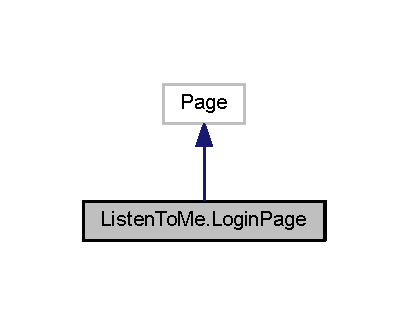
\includegraphics[width=196pt]{class_listen_to_me_1_1_login_page__inherit__graph}
\end{center}
\end{figure}
\subsection*{Public Member Functions}
\begin{DoxyCompactItemize}
\item 
\mbox{\hyperlink{class_listen_to_me_1_1_login_page_afcefc5f9f4f5cee5d9f5e15493e4058b}{Login\+Page}} ()
\begin{DoxyCompactList}\small\item\em names the resourcename for the passwordvault. \end{DoxyCompactList}\end{DoxyCompactItemize}
\subsection*{Private Member Functions}
\begin{DoxyCompactItemize}
\item 
async void \mbox{\hyperlink{class_listen_to_me_1_1_login_page_ace57aa2c75a95bab9c32ea95bc9adb31}{Login\+Button\+\_\+\+Click\+Async}} (object sender, Routed\+Event\+Args e)
\begin{DoxyCompactList}\small\item\em calls some valigation rules based on length that are similar to the buisiness logic behind the webform \end{DoxyCompactList}\item 
void \mbox{\hyperlink{class_listen_to_me_1_1_login_page_a3f7972af36ca0c72f1bd37c4a3f84c14}{Switch\+To\+Next\+Page}} ()
\begin{DoxyCompactList}\small\item\em navigates the frame if logged in sucessfully \end{DoxyCompactList}\end{DoxyCompactItemize}
\subsection*{Static Private Member Functions}
\begin{DoxyCompactItemize}
\item 
static void \mbox{\hyperlink{class_listen_to_me_1_1_login_page_af6692799b00ea2ad405a7af8dff73ad3}{Add\+User\+Credential}} (string username, string password)
\begin{DoxyCompactList}\small\item\em adds a user credential to the password vault \end{DoxyCompactList}\end{DoxyCompactItemize}


\subsection{Detailed Description}
retrieves and stores login Information in a password vault to\+Do\+: use this for direct\+Line secret as well 



\subsection{Constructor \& Destructor Documentation}
\mbox{\Hypertarget{class_listen_to_me_1_1_login_page_afcefc5f9f4f5cee5d9f5e15493e4058b}\label{class_listen_to_me_1_1_login_page_afcefc5f9f4f5cee5d9f5e15493e4058b}} 
\index{Listen\+To\+Me\+::\+Login\+Page@{Listen\+To\+Me\+::\+Login\+Page}!Login\+Page@{Login\+Page}}
\index{Login\+Page@{Login\+Page}!Listen\+To\+Me\+::\+Login\+Page@{Listen\+To\+Me\+::\+Login\+Page}}
\subsubsection{\texorpdfstring{Login\+Page()}{LoginPage()}}
{\footnotesize\ttfamily Listen\+To\+Me.\+Login\+Page.\+Login\+Page (\begin{DoxyParamCaption}{ }\end{DoxyParamCaption})}



names the resourcename for the passwordvault. 

retreives the credentials from the list and populates the G\+UI with them, sets the cursor 

\subsection{Member Function Documentation}
\mbox{\Hypertarget{class_listen_to_me_1_1_login_page_af6692799b00ea2ad405a7af8dff73ad3}\label{class_listen_to_me_1_1_login_page_af6692799b00ea2ad405a7af8dff73ad3}} 
\index{Listen\+To\+Me\+::\+Login\+Page@{Listen\+To\+Me\+::\+Login\+Page}!Add\+User\+Credential@{Add\+User\+Credential}}
\index{Add\+User\+Credential@{Add\+User\+Credential}!Listen\+To\+Me\+::\+Login\+Page@{Listen\+To\+Me\+::\+Login\+Page}}
\subsubsection{\texorpdfstring{Add\+User\+Credential()}{AddUserCredential()}}
{\footnotesize\ttfamily static void Listen\+To\+Me.\+Login\+Page.\+Add\+User\+Credential (\begin{DoxyParamCaption}\item[{string}]{username,  }\item[{string}]{password }\end{DoxyParamCaption})\hspace{0.3cm}{\ttfamily [static]}, {\ttfamily [private]}}



adds a user credential to the password vault 


\begin{DoxyParams}{Parameters}
{\em username} & the username of the credential\\
\hline
{\em password} & the password of the credential\\
\hline
\end{DoxyParams}
\mbox{\Hypertarget{class_listen_to_me_1_1_login_page_ace57aa2c75a95bab9c32ea95bc9adb31}\label{class_listen_to_me_1_1_login_page_ace57aa2c75a95bab9c32ea95bc9adb31}} 
\index{Listen\+To\+Me\+::\+Login\+Page@{Listen\+To\+Me\+::\+Login\+Page}!Login\+Button\+\_\+\+Click\+Async@{Login\+Button\+\_\+\+Click\+Async}}
\index{Login\+Button\+\_\+\+Click\+Async@{Login\+Button\+\_\+\+Click\+Async}!Listen\+To\+Me\+::\+Login\+Page@{Listen\+To\+Me\+::\+Login\+Page}}
\subsubsection{\texorpdfstring{Login\+Button\+\_\+\+Click\+Async()}{LoginButton\_ClickAsync()}}
{\footnotesize\ttfamily async void Listen\+To\+Me.\+Login\+Page.\+Login\+Button\+\_\+\+Click\+Async (\begin{DoxyParamCaption}\item[{object}]{sender,  }\item[{Routed\+Event\+Args}]{e }\end{DoxyParamCaption})\hspace{0.3cm}{\ttfamily [private]}}



calls some valigation rules based on length that are similar to the buisiness logic behind the webform 


\begin{DoxyParams}{Parameters}
{\em sender} & the button\\
\hline
{\em e} & event information\\
\hline
\end{DoxyParams}
\mbox{\Hypertarget{class_listen_to_me_1_1_login_page_a3f7972af36ca0c72f1bd37c4a3f84c14}\label{class_listen_to_me_1_1_login_page_a3f7972af36ca0c72f1bd37c4a3f84c14}} 
\index{Listen\+To\+Me\+::\+Login\+Page@{Listen\+To\+Me\+::\+Login\+Page}!Switch\+To\+Next\+Page@{Switch\+To\+Next\+Page}}
\index{Switch\+To\+Next\+Page@{Switch\+To\+Next\+Page}!Listen\+To\+Me\+::\+Login\+Page@{Listen\+To\+Me\+::\+Login\+Page}}
\subsubsection{\texorpdfstring{Switch\+To\+Next\+Page()}{SwitchToNextPage()}}
{\footnotesize\ttfamily void Listen\+To\+Me.\+Login\+Page.\+Switch\+To\+Next\+Page (\begin{DoxyParamCaption}{ }\end{DoxyParamCaption})\hspace{0.3cm}{\ttfamily [private]}}



navigates the frame if logged in sucessfully 



The documentation for this class was generated from the following file\+:\begin{DoxyCompactItemize}
\item 
C\+:/\+Users/fgeissle/source/repos/\+F\+B\+K\+Voice\+App/\+Listen\+To\+Me/\mbox{\hyperlink{_login_page_8xaml_8cs}{Login\+Page.\+xaml.\+cs}}\end{DoxyCompactItemize}

\hypertarget{class_listen_to_me_1_1_main_page}{}\section{Listen\+To\+Me.\+Main\+Page Class Reference}
\label{class_listen_to_me_1_1_main_page}\index{Listen\+To\+Me.\+Main\+Page@{Listen\+To\+Me.\+Main\+Page}}


The class \hyperlink{class_listen_to_me_1_1_main_page}{Main\+Page} contains the navigation buttons of the app as well as the speech input field  




Inheritance diagram for Listen\+To\+Me.\+Main\+Page\+:
\nopagebreak
\begin{figure}[H]
\begin{center}
\leavevmode
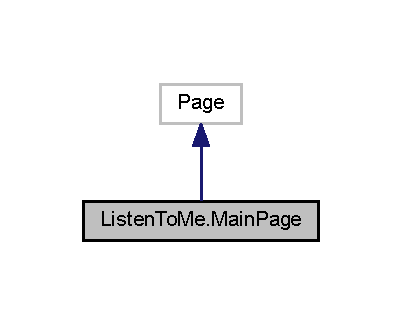
\includegraphics[width=193pt]{class_listen_to_me_1_1_main_page__inherit__graph}
\end{center}
\end{figure}


Collaboration diagram for Listen\+To\+Me.\+Main\+Page\+:
\nopagebreak
\begin{figure}[H]
\begin{center}
\leavevmode
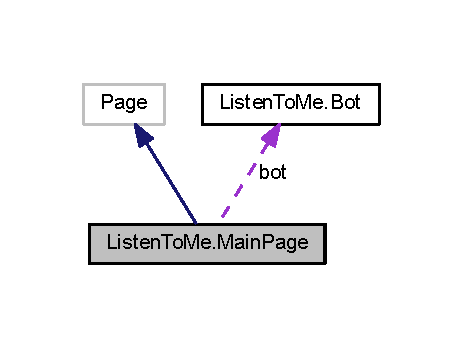
\includegraphics[width=222pt]{class_listen_to_me_1_1_main_page__coll__graph}
\end{center}
\end{figure}
\subsection*{Public Member Functions}
\begin{DoxyCompactItemize}
\item 
\hyperlink{class_listen_to_me_1_1_main_page_afb2ff548c6284f6f179fc9b3dcc89245}{Main\+Page} ()
\item 
async void \hyperlink{class_listen_to_me_1_1_main_page_a4adb881a143354b71604cfa79ea69e25}{test\+Net\+Connection\+Smaller} ()
\begin{DoxyCompactList}\small\item\em testing connection to the website. Not working, both requests return with empty responses. reference\+: \href{https://blogs.windows.com/buildingapps/2015/11/23/demystifying-httpclient-apis-in-the-universal-windows-platform/#kzmsLAKtjKLGJFAU.97}{\tt https\+://blogs.\+windows.\+com/buildingapps/2015/11/23/demystifying-\/httpclient-\/apis-\/in-\/the-\/universal-\/windows-\/platform/\#kzms\+L\+A\+Ktj\+K\+L\+G\+J\+F\+A\+U.\+97} reference\+: \href{https://docs.microsoft.com/en-us/aspnet/web-api/overview/advanced/calling-a-web-api-from-a-net-client}{\tt https\+://docs.\+microsoft.\+com/en-\/us/aspnet/web-\/api/overview/advanced/calling-\/a-\/web-\/api-\/from-\/a-\/net-\/client} \end{DoxyCompactList}\end{DoxyCompactItemize}
\subsection*{Static Public Member Functions}
\begin{DoxyCompactItemize}
\item 
static string \hyperlink{class_listen_to_me_1_1_main_page_af4469348ffee9a5d1a8680d2535a279b}{First\+Char\+To\+Upper} (string input)
\begin{DoxyCompactList}\small\item\em helper method for cleaning output from luis. Since L\+U\+IS answers in lowercase only, this method uppercases the first letter \end{DoxyCompactList}\end{DoxyCompactItemize}
\subsection*{Public Attributes}
\begin{DoxyCompactItemize}
\item 
bool \hyperlink{class_listen_to_me_1_1_main_page_a03679610fded2c61480540ebcc7e4667}{show\+Grid}
\begin{DoxyCompactList}\small\item\em storing wether the grid is visible for grid navigation \end{DoxyCompactList}\end{DoxyCompactItemize}
\subsection*{Protected Member Functions}
\begin{DoxyCompactItemize}
\item 
override async void \hyperlink{class_listen_to_me_1_1_main_page_a8027d1a18b781cfe127ca02916c4552e}{On\+Navigated\+To} (Navigation\+Event\+Args e)
\begin{DoxyCompactList}\small\item\em is called after the login was sucessful \end{DoxyCompactList}\item 
override void \hyperlink{class_listen_to_me_1_1_main_page_a15a008ef01c6354ef72d4ec864d8d8e3}{On\+Navigated\+From} (Navigation\+Event\+Args e)
\end{DoxyCompactItemize}
\subsection*{Private Member Functions}
\begin{DoxyCompactItemize}
\item 
async void \hyperlink{class_listen_to_me_1_1_main_page_ae285c1eb3d44999ceecdb1b4f5a7bf83}{test\+Regex} ()
\item 
async void \hyperlink{class_listen_to_me_1_1_main_page_a781bed1ae1145079c62597b5a938c0d1}{init\+Frame} ()
\begin{DoxyCompactList}\small\item\em fills the section field in formstore with information from the web form \end{DoxyCompactList}\item 
void \hyperlink{class_listen_to_me_1_1_main_page_abd810ebce6d7300369767bd604e107d2}{navigation\+Helper\+\_\+\+Save\+State} (object sender, Save\+State\+Event\+Args e)
\begin{DoxyCompactList}\small\item\em to\+Do implement formstore call that saves the values of the input fields \end{DoxyCompactList}\item 
void \hyperlink{class_listen_to_me_1_1_main_page_a696e8f4cb397c01ba2465d68e2b8c369}{navigation\+Helper\+\_\+\+Load\+State} (object sender, Load\+State\+Event\+Args e)
\begin{DoxyCompactList}\small\item\em to\+Do implement formstore call that loads the values of the input fields \end{DoxyCompactList}\item 
async Task$<$ string $>$ \hyperlink{class_listen_to_me_1_1_main_page_ab68e25e8370c434b0deb5069c7cdd254}{determine\+Response} (string intent, string text\+Value, string users\+Field\+Name, string luis\+Type\+Of\+Text\+Value)
\begin{DoxyCompactList}\small\item\em is essential in processing the recognized L\+U\+I\+S-\/entities. Sometimes L\+U\+IS entities are not recognized by the language model. \end{DoxyCompactList}\item 
void \hyperlink{class_listen_to_me_1_1_main_page_a465e7f9723aec19e912a3913841d477e}{Clicked} (string sender, string text\+Value)
\item 
async Task \hyperlink{class_listen_to_me_1_1_main_page_adbf1a6a0cab368d6e803bbd1b918a045}{Init\+Continuous\+Recognition} ()
\begin{DoxyCompactList}\small\item\em sets up continous speech recognition \end{DoxyCompactList}\item 
async void \hyperlink{class_listen_to_me_1_1_main_page_afad060c55f3bedc7d8e499829e133c98}{Continuous\+Recognition\+Session\+\_\+\+Result\+Generated} (Speech\+Continuous\+Recognition\+Session sender, Speech\+Continuous\+Recognition\+Result\+Generated\+Event\+Args args)
\item 
void \hyperlink{class_listen_to_me_1_1_main_page_ab7c9aeb7a6b1053375754c58933360d6}{Media\+\_\+\+Media\+Ended} (object sender, Routed\+Event\+Args e)
\item 
void \hyperlink{class_listen_to_me_1_1_main_page_a9e7a645ae278f0e83ff9c3a831b37028}{Page\+\_\+\+Loaded} (object sender, Routed\+Event\+Args e)
\item 
async void \hyperlink{class_listen_to_me_1_1_main_page_ad477d18baff88094baa32ac20b462284}{Back\+Button\+\_\+\+Click} (object sender, Routed\+Event\+Args e)
\item 
async Task \hyperlink{class_listen_to_me_1_1_main_page_a1ccf14d59eabbcc4148cadd8dd11fc04}{go\+Back\+Async} ()
\item 
async Task \hyperlink{class_listen_to_me_1_1_main_page_a1a1e1d6e362134f6426bcf99ca83c45c}{fill\+Frame\+Async} ()
\begin{DoxyCompactList}\small\item\em fill Frame creates a new Page for main\+Frame and adds it to the main\+Frame as Content \end{DoxyCompactList}\item 
async Task \hyperlink{class_listen_to_me_1_1_main_page_a16241dfda10c37812bcb3a55a791e011}{create\+Section} (Section section, Stack\+Panel my\+Panel)
\begin{DoxyCompactList}\small\item\em creates a section by adding control elements to a panel \end{DoxyCompactList}\item 
async Task \hyperlink{class_listen_to_me_1_1_main_page_a73b3a3311149846cf028c5824dab2a6e}{Create\+Element\+Async} (Element element, Stack\+Panel panel, Text\+Box field=null)
\begin{DoxyCompactList}\small\item\em creates an element from the section object by determining what type of element it is reference\+: \href{https://stackoverflow.com/questions/37297810/updatesourcetrigger-dont-work-in-wpf-customcontrols}{\tt https\+://stackoverflow.\+com/questions/37297810/updatesourcetrigger-\/dont-\/work-\/in-\/wpf-\/customcontrols} \end{DoxyCompactList}\item 
void \hyperlink{class_listen_to_me_1_1_main_page_a80911257473f608abc125a1083045041}{set\+Enabled\+And\+Hash\+For\+Field} (Text\+Box field, Element element, Stack\+Panel panel)
\begin{DoxyCompactList}\small\item\em sets the enabled property of a Text\+Box control to disabled, if the model Element\textquotesingle{}s property is set to \textquotesingle{}disabled\textquotesingle{} string. This is the case for input elements that are only for displaying information, e.\+g. summing up other entries made by the user. If the Text\+Box stays enabled, the header will be added to the Hash\+Table that is used by the L\+U\+I\+S-\/\+Model to determine to which Text\+Box to pass a user value to. \end{DoxyCompactList}\item 
async void \hyperlink{class_listen_to_me_1_1_main_page_a4dec5880c4a900edea6e9a2f37cd93fc}{Home\+Button\+\_\+\+Click} (object sender, Routed\+Event\+Args e)
\begin{DoxyCompactList}\small\item\em has no speacial meaning as of yet \end{DoxyCompactList}\item 
async void \hyperlink{class_listen_to_me_1_1_main_page_a8144f2438fc2512708677190d74d2111}{Next\+Button\+\_\+\+Click} (object sender, Routed\+Event\+Args e)
\begin{DoxyCompactList}\small\item\em loads the next section into the frame \end{DoxyCompactList}\item 
async Task \hyperlink{class_listen_to_me_1_1_main_page_a8cd1a04a404800cfab55de0ba4466f68}{go\+Next\+Async} ()
\item 
void \hyperlink{class_listen_to_me_1_1_main_page_acad3fb1a64c0bea077f5ad38627faeef}{dynamic\+Button\+\_\+\+Click} (object sender, Routed\+Event\+Args e)
\begin{DoxyCompactList}\small\item\em Button is hit for microphone activation \end{DoxyCompactList}\item 
async void \hyperlink{class_listen_to_me_1_1_main_page_afee59bda6fcfb361bf088d543e197879}{button\+\_\+\+Click} (object sender, Routed\+Event\+Args e)
\begin{DoxyCompactList}\small\item\em Button is hit for microphone activation \end{DoxyCompactList}\item 
async System.\+Threading.\+Tasks.\+Task \hyperlink{class_listen_to_me_1_1_main_page_a57d75ef6bb9c10b0c944c3eb5513b076}{Set\+Listening\+Async} (bool to\+Listen)
\begin{DoxyCompactList}\small\item\em sets the flag whether speech recognition is enabled according to the parameter \end{DoxyCompactList}\item 
async void \hyperlink{class_listen_to_me_1_1_main_page_ab9fba04f0fc94773c2838f6af87ec14b}{Start\+Listen\+Mode} ()
\begin{DoxyCompactList}\small\item\em analyzes the speech input, recognized the text and calls \hyperlink{class_listen_to_me_1_1_main_page_a09c2518852d4261ff6a2118c8e01de9f}{Send\+Message()} to display the rcognized text \end{DoxyCompactList}\item 
async void \hyperlink{class_listen_to_me_1_1_main_page_a09c2518852d4261ff6a2118c8e01de9f}{Send\+Message} (string message, bool speak=false)
\begin{DoxyCompactList}\small\item\em calls the L\+U\+IS A\+PI to retrieve the \hyperlink{class_listen_to_me_1_1_bot}{Bot} Web\+App\textquotesingle{}s answer for a specific request \end{DoxyCompactList}\item 
async void \hyperlink{class_listen_to_me_1_1_main_page_a203cee0f97f99d3ac38d9338e7c39427}{check\+Other\+Intents} (string intent, string message, bool speak)
\begin{DoxyCompactList}\small\item\em helps calling actions of intents other than Field.\+Fill\+In \end{DoxyCompactList}\item 
async Task \hyperlink{class_listen_to_me_1_1_main_page_aa1c50f04230b8907027a95bfe54cb7d2}{Speak\+Async} (string to\+Speak)
\begin{DoxyCompactList}\small\item\em lets the \hyperlink{class_listen_to_me_1_1_app}{App} speak the answer to the user \end{DoxyCompactList}\item 
async Task$<$ string $>$ \hyperlink{class_listen_to_me_1_1_main_page_a94a7dfd5dc1ec2e9bf7a86a4b9f7df0c}{Listen\+For\+Text} ()
\begin{DoxyCompactList}\small\item\em handles exceptions in the speechrecognition api. Also checks whether the device the user in using has enabled microphone input \end{DoxyCompactList}\item 
async Task \hyperlink{class_listen_to_me_1_1_main_page_ac541bec23372af9da39117384c6b177e}{Init\+Speech} ()
\begin{DoxyCompactList}\small\item\em initialized speech recognition \end{DoxyCompactList}\item 
async void \hyperlink{class_listen_to_me_1_1_main_page_a78024cb9b68bafc3375081574dbbea89}{Speech\+Recognizer\+\_\+\+Hypothesis\+Generated} (Speech\+Recognizer sender, Speech\+Recognition\+Hypothesis\+Generated\+Event\+Args args)
\begin{DoxyCompactList}\small\item\em handles the Hypothesis\+Generated event of the speech recognizer \end{DoxyCompactList}\item 
void \hyperlink{class_listen_to_me_1_1_main_page_a2b101dc0c72c1dcb73fe756a5847940e}{text\+\_\+\+Key\+Down} (object sender, Key\+Routed\+Event\+Args e)
\begin{DoxyCompactList}\small\item\em Method that is reacting each time a key is hit while the textinput field has focus. \end{DoxyCompactList}\end{DoxyCompactItemize}
\subsection*{Private Attributes}
\begin{DoxyCompactItemize}
\item 
Navigation\+Helper \hyperlink{class_listen_to_me_1_1_main_page_a9ad9fdc2f7159cbe2d495645459cffe8}{navigation\+Helper}
\begin{DoxyCompactList}\small\item\em Navigationhelper is administrating the history of the pages in the frame of the programm \end{DoxyCompactList}\item 
Navigation\+Service \hyperlink{class_listen_to_me_1_1_main_page_aff60f67b7f65b20f4df33be26d015bcf}{navigation\+Service}
\begin{DoxyCompactList}\small\item\em navigation\+Service is controlling the rootframe changes whenever navigation occurs \end{DoxyCompactList}\item 
bool \hyperlink{class_listen_to_me_1_1_main_page_ad46f69d6d70b9b13b74b4013b86ca608}{listening} = false
\begin{DoxyCompactList}\small\item\em a variable that is true when the user is speaking to the speech input field and false if he is typing into the speech input field \end{DoxyCompactList}\item 
Root\+Frame\+Navigation\+Helper \hyperlink{class_listen_to_me_1_1_main_page_a3185b88ec21f447708a2d3da983997e0}{my\+Frame\+Helper}
\begin{DoxyCompactList}\small\item\em rootframe navigation helper is helping the rootframe navigation with keyboard events \end{DoxyCompactList}\item 
Speech\+Recognizer \hyperlink{class_listen_to_me_1_1_main_page_ac417ca2ffe02d44895c029bf23e8f83a}{speech\+Recognizer\+Continuous}
\begin{DoxyCompactList}\small\item\em evaluates speech input if the user is continually speaking. triggered by the user saying start listening. If the command stop listening is said, it will stop continous speech recognition \end{DoxyCompactList}\item 
\hyperlink{class_listen_to_me_1_1_bot}{Bot} \hyperlink{class_listen_to_me_1_1_main_page_a09b9deff7e80e3d524cd0f12d1c060f9}{bot}
\begin{DoxyCompactList}\small\item\em connects via Direct\+Line tho the Web\+App. Communicates with the language understanding intelligence model \end{DoxyCompactList}\item 
Resource\+Loader \hyperlink{class_listen_to_me_1_1_main_page_a906eb7f1e61084dcfb0b0f833b0d96f4}{loader}
\begin{DoxyCompactList}\small\item\em loads localized string ressources from Strings/ directory \end{DoxyCompactList}\item 
int \hyperlink{class_listen_to_me_1_1_main_page_a94ae31ea5ea90fff0194c7c3345e3987}{count\+User\+Inputs}
\begin{DoxyCompactList}\small\item\em counts the user\textquotesingle{}s inputs for helping the app at guessing which field is filled out next. \end{DoxyCompactList}\item 
Speech\+Recognizer \hyperlink{class_listen_to_me_1_1_main_page_a56393ec41c67e438e12651f5dc44a2cc}{speech\+Recognizer}
\begin{DoxyCompactList}\small\item\em evaluates speech input if the user is only speaking a defined interval (e.\+g while speech input button is pressed) \end{DoxyCompactList}\item 
Manual\+Reset\+Event \hyperlink{class_listen_to_me_1_1_main_page_acc2116e019bacfa54fd25381eeaf363f}{manual\+Reset\+Event}
\begin{DoxyCompactList}\small\item\em has no tasks so far but might be important in the future \end{DoxyCompactList}\item 
int \hyperlink{class_listen_to_me_1_1_main_page_afa885f51f46e84b050d0874e64389880}{pages\+Count}
\begin{DoxyCompactList}\small\item\em variable that counts the sections to know which section has to be loades into the frame \end{DoxyCompactList}\item 
Stack\+Panel \hyperlink{class_listen_to_me_1_1_main_page_a6dbd09c74d99bf0223489a06035980eb}{current\+Panel}
\begin{DoxyCompactList}\small\item\em contains the Text\+Boxes and other controls of the page \end{DoxyCompactList}\item 
int \hyperlink{class_listen_to_me_1_1_main_page_acc0f3cb24ff26c2cfc76cd42a2fe2118}{index\+Of\+Current\+Element}
\begin{DoxyCompactList}\small\item\em index of the last Text\+Box to which text was send with \hyperlink{class_listen_to_me_1_1_main_page_a09c2518852d4261ff6a2118c8e01de9f}{Send\+Message(string, bool)} \end{DoxyCompactList}\item 
List$<$ string $>$ \hyperlink{class_listen_to_me_1_1_main_page_a7ee97019c1b3318631a799c2979b7364}{inputs}
\item 
bool \hyperlink{class_listen_to_me_1_1_main_page_a448f51804566fe32efca61994caf9ab9}{Is\+Initializing} = true
\begin{DoxyCompactList}\small\item\em flag for preventing the \hyperlink{class_listen_to_me_1_1_main_page_a465e7f9723aec19e912a3913841d477e}{Clicked(string, string)} \end{DoxyCompactList}\end{DoxyCompactItemize}


\subsection{Detailed Description}
The class \hyperlink{class_listen_to_me_1_1_main_page}{Main\+Page} contains the navigation buttons of the app as well as the speech input field 



\subsection{Constructor \& Destructor Documentation}
\index{Listen\+To\+Me\+::\+Main\+Page@{Listen\+To\+Me\+::\+Main\+Page}!Main\+Page@{Main\+Page}}
\index{Main\+Page@{Main\+Page}!Listen\+To\+Me\+::\+Main\+Page@{Listen\+To\+Me\+::\+Main\+Page}}
\subsubsection[{\texorpdfstring{Main\+Page()}{MainPage()}}]{\setlength{\rightskip}{0pt plus 5cm}Listen\+To\+Me.\+Main\+Page.\+Main\+Page (
\begin{DoxyParamCaption}
{}
\end{DoxyParamCaption}
)}\hypertarget{class_listen_to_me_1_1_main_page_afb2ff548c6284f6f179fc9b3dcc89245}{}\label{class_listen_to_me_1_1_main_page_afb2ff548c6284f6f179fc9b3dcc89245}


Here is the call graph for this function\+:
\nopagebreak
\begin{figure}[H]
\begin{center}
\leavevmode
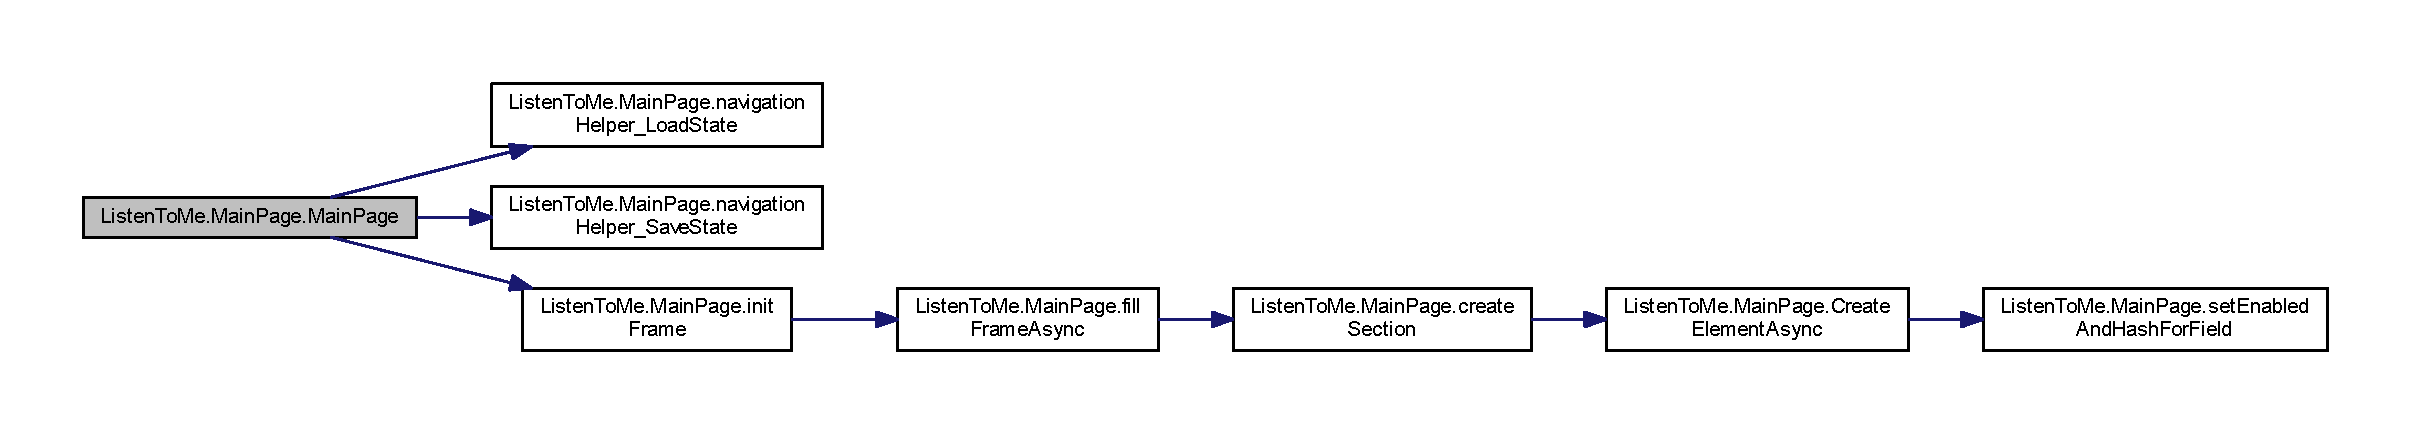
\includegraphics[width=350pt]{class_listen_to_me_1_1_main_page_afb2ff548c6284f6f179fc9b3dcc89245_cgraph}
\end{center}
\end{figure}




\subsection{Member Function Documentation}
\index{Listen\+To\+Me\+::\+Main\+Page@{Listen\+To\+Me\+::\+Main\+Page}!Back\+Button\+\_\+\+Click@{Back\+Button\+\_\+\+Click}}
\index{Back\+Button\+\_\+\+Click@{Back\+Button\+\_\+\+Click}!Listen\+To\+Me\+::\+Main\+Page@{Listen\+To\+Me\+::\+Main\+Page}}
\subsubsection[{\texorpdfstring{Back\+Button\+\_\+\+Click(object sender, Routed\+Event\+Args e)}{BackButton_Click(object sender, RoutedEventArgs e)}}]{\setlength{\rightskip}{0pt plus 5cm}async void Listen\+To\+Me.\+Main\+Page.\+Back\+Button\+\_\+\+Click (
\begin{DoxyParamCaption}
\item[{object}]{sender, }
\item[{Routed\+Event\+Args}]{e}
\end{DoxyParamCaption}
)\hspace{0.3cm}{\ttfamily [private]}}\hypertarget{class_listen_to_me_1_1_main_page_ad477d18baff88094baa32ac20b462284}{}\label{class_listen_to_me_1_1_main_page_ad477d18baff88094baa32ac20b462284}


Here is the call graph for this function\+:
\nopagebreak
\begin{figure}[H]
\begin{center}
\leavevmode
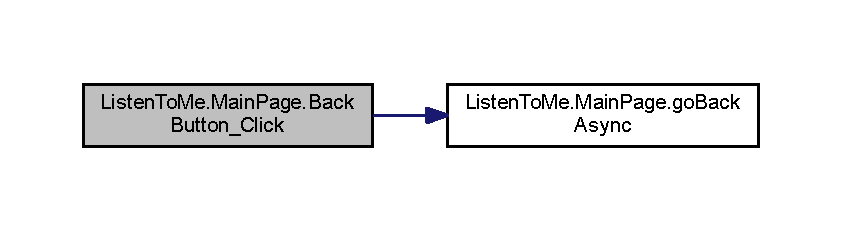
\includegraphics[width=350pt]{class_listen_to_me_1_1_main_page_ad477d18baff88094baa32ac20b462284_cgraph}
\end{center}
\end{figure}


\index{Listen\+To\+Me\+::\+Main\+Page@{Listen\+To\+Me\+::\+Main\+Page}!button\+\_\+\+Click@{button\+\_\+\+Click}}
\index{button\+\_\+\+Click@{button\+\_\+\+Click}!Listen\+To\+Me\+::\+Main\+Page@{Listen\+To\+Me\+::\+Main\+Page}}
\subsubsection[{\texorpdfstring{button\+\_\+\+Click(object sender, Routed\+Event\+Args e)}{button_Click(object sender, RoutedEventArgs e)}}]{\setlength{\rightskip}{0pt plus 5cm}async void Listen\+To\+Me.\+Main\+Page.\+button\+\_\+\+Click (
\begin{DoxyParamCaption}
\item[{object}]{sender, }
\item[{Routed\+Event\+Args}]{e}
\end{DoxyParamCaption}
)\hspace{0.3cm}{\ttfamily [private]}}\hypertarget{class_listen_to_me_1_1_main_page_afee59bda6fcfb361bf088d543e197879}{}\label{class_listen_to_me_1_1_main_page_afee59bda6fcfb361bf088d543e197879}


Button is hit for microphone activation 


\begin{DoxyParams}{Parameters}
{\em sender} & the microphone button\\
\hline
{\em e} & some eventarguments\\
\hline
\end{DoxyParams}


Here is the call graph for this function\+:
\nopagebreak
\begin{figure}[H]
\begin{center}
\leavevmode
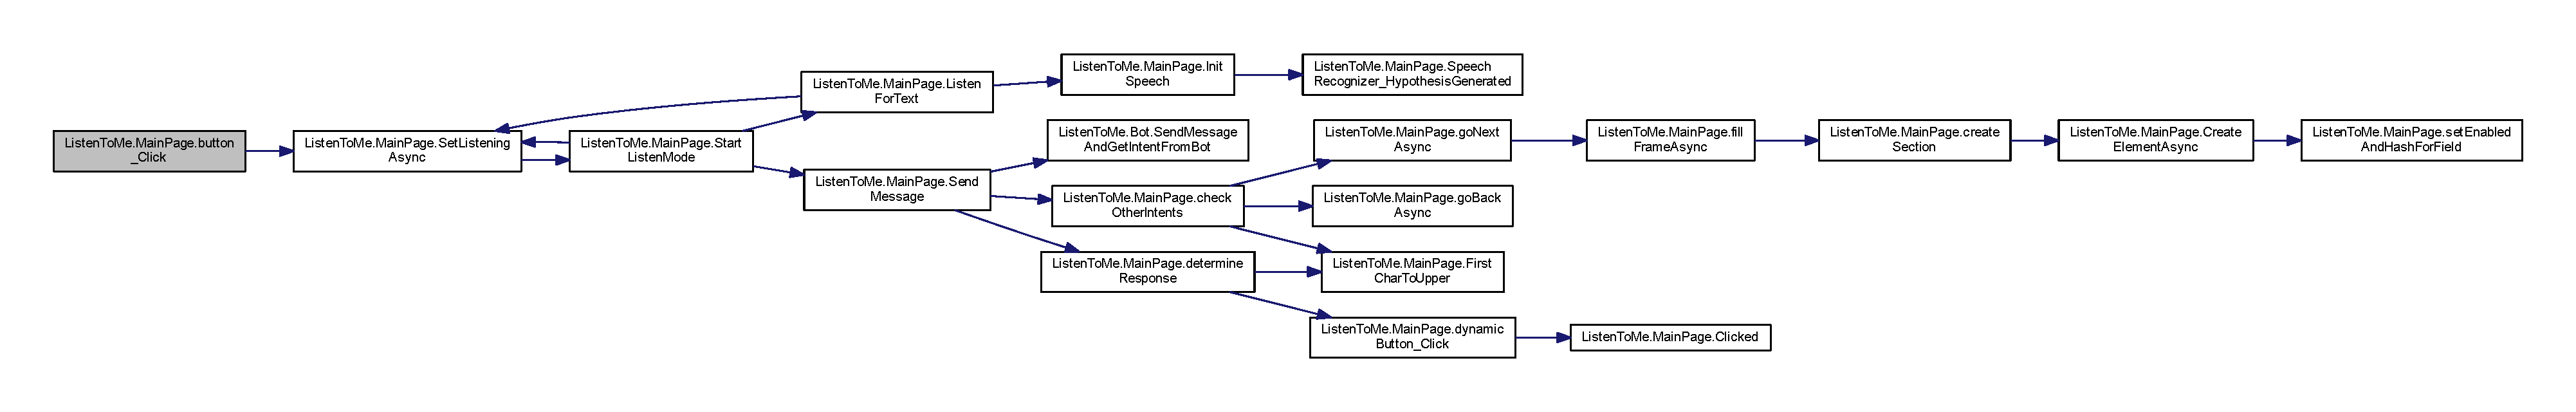
\includegraphics[width=350pt]{class_listen_to_me_1_1_main_page_afee59bda6fcfb361bf088d543e197879_cgraph}
\end{center}
\end{figure}


\index{Listen\+To\+Me\+::\+Main\+Page@{Listen\+To\+Me\+::\+Main\+Page}!check\+Other\+Intents@{check\+Other\+Intents}}
\index{check\+Other\+Intents@{check\+Other\+Intents}!Listen\+To\+Me\+::\+Main\+Page@{Listen\+To\+Me\+::\+Main\+Page}}
\subsubsection[{\texorpdfstring{check\+Other\+Intents(string intent, string message, bool speak)}{checkOtherIntents(string intent, string message, bool speak)}}]{\setlength{\rightskip}{0pt plus 5cm}async void Listen\+To\+Me.\+Main\+Page.\+check\+Other\+Intents (
\begin{DoxyParamCaption}
\item[{string}]{intent, }
\item[{string}]{message, }
\item[{bool}]{speak}
\end{DoxyParamCaption}
)\hspace{0.3cm}{\ttfamily [private]}}\hypertarget{class_listen_to_me_1_1_main_page_a203cee0f97f99d3ac38d9338e7c39427}{}\label{class_listen_to_me_1_1_main_page_a203cee0f97f99d3ac38d9338e7c39427}


helps calling actions of intents other than Field.\+Fill\+In 


\begin{DoxyParams}{Parameters}
{\em intent} & the name of the intent\\
\hline
\end{DoxyParams}


Here is the call graph for this function\+:
\nopagebreak
\begin{figure}[H]
\begin{center}
\leavevmode
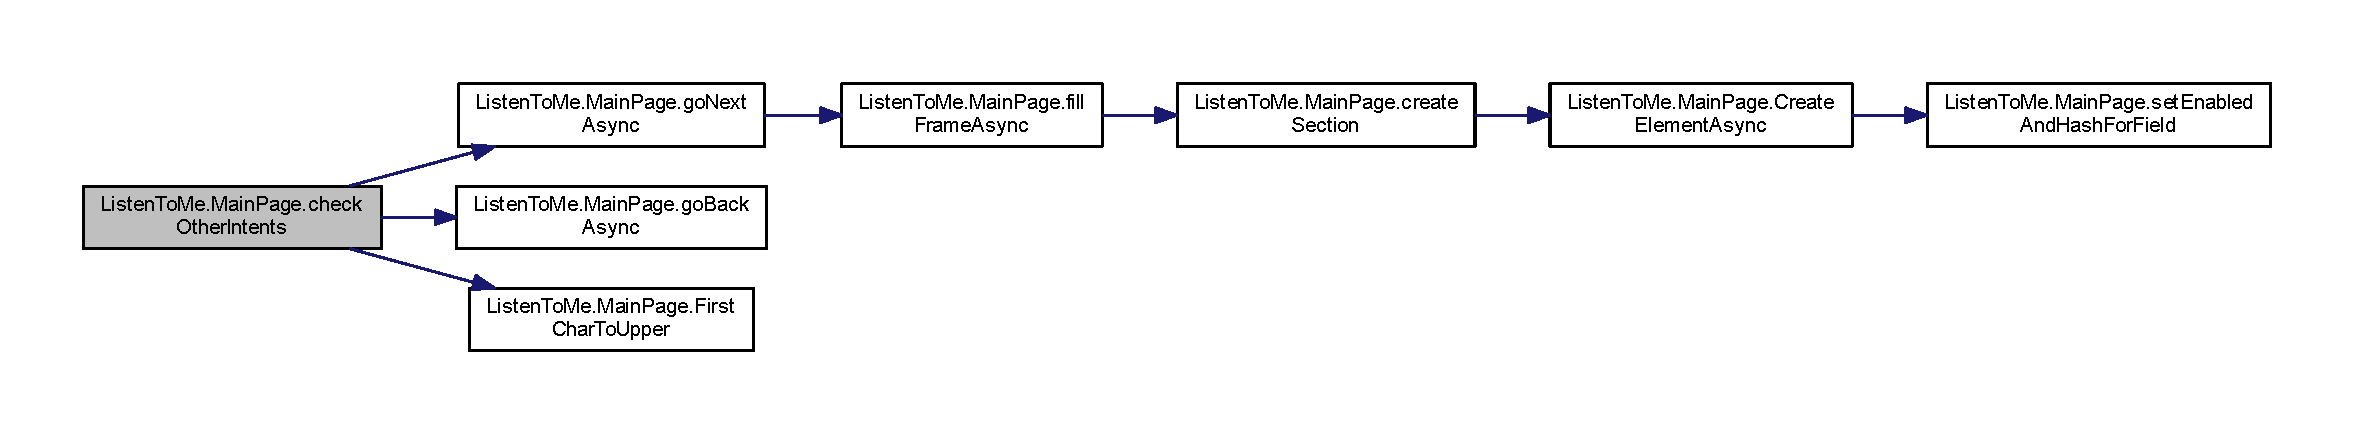
\includegraphics[width=350pt]{class_listen_to_me_1_1_main_page_a203cee0f97f99d3ac38d9338e7c39427_cgraph}
\end{center}
\end{figure}




Here is the caller graph for this function\+:
\nopagebreak
\begin{figure}[H]
\begin{center}
\leavevmode
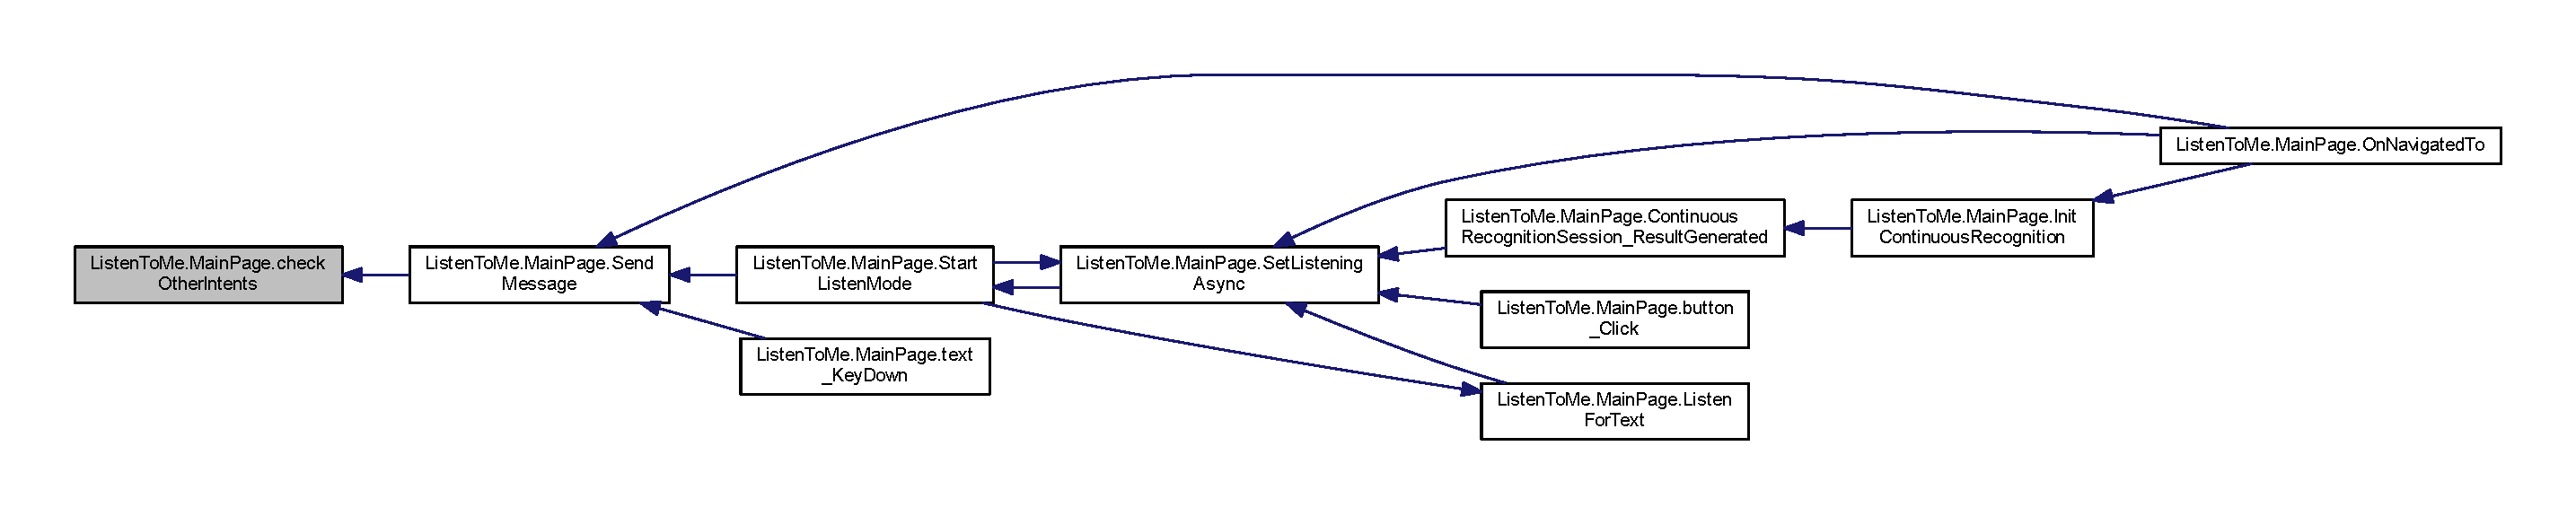
\includegraphics[width=350pt]{class_listen_to_me_1_1_main_page_a203cee0f97f99d3ac38d9338e7c39427_icgraph}
\end{center}
\end{figure}


\index{Listen\+To\+Me\+::\+Main\+Page@{Listen\+To\+Me\+::\+Main\+Page}!Clicked@{Clicked}}
\index{Clicked@{Clicked}!Listen\+To\+Me\+::\+Main\+Page@{Listen\+To\+Me\+::\+Main\+Page}}
\subsubsection[{\texorpdfstring{Clicked(string sender, string text\+Value)}{Clicked(string sender, string textValue)}}]{\setlength{\rightskip}{0pt plus 5cm}void Listen\+To\+Me.\+Main\+Page.\+Clicked (
\begin{DoxyParamCaption}
\item[{string}]{sender, }
\item[{string}]{text\+Value}
\end{DoxyParamCaption}
)\hspace{0.3cm}{\ttfamily [private]}}\hypertarget{class_listen_to_me_1_1_main_page_a465e7f9723aec19e912a3913841d477e}{}\label{class_listen_to_me_1_1_main_page_a465e7f9723aec19e912a3913841d477e}


Here is the caller graph for this function\+:
\nopagebreak
\begin{figure}[H]
\begin{center}
\leavevmode
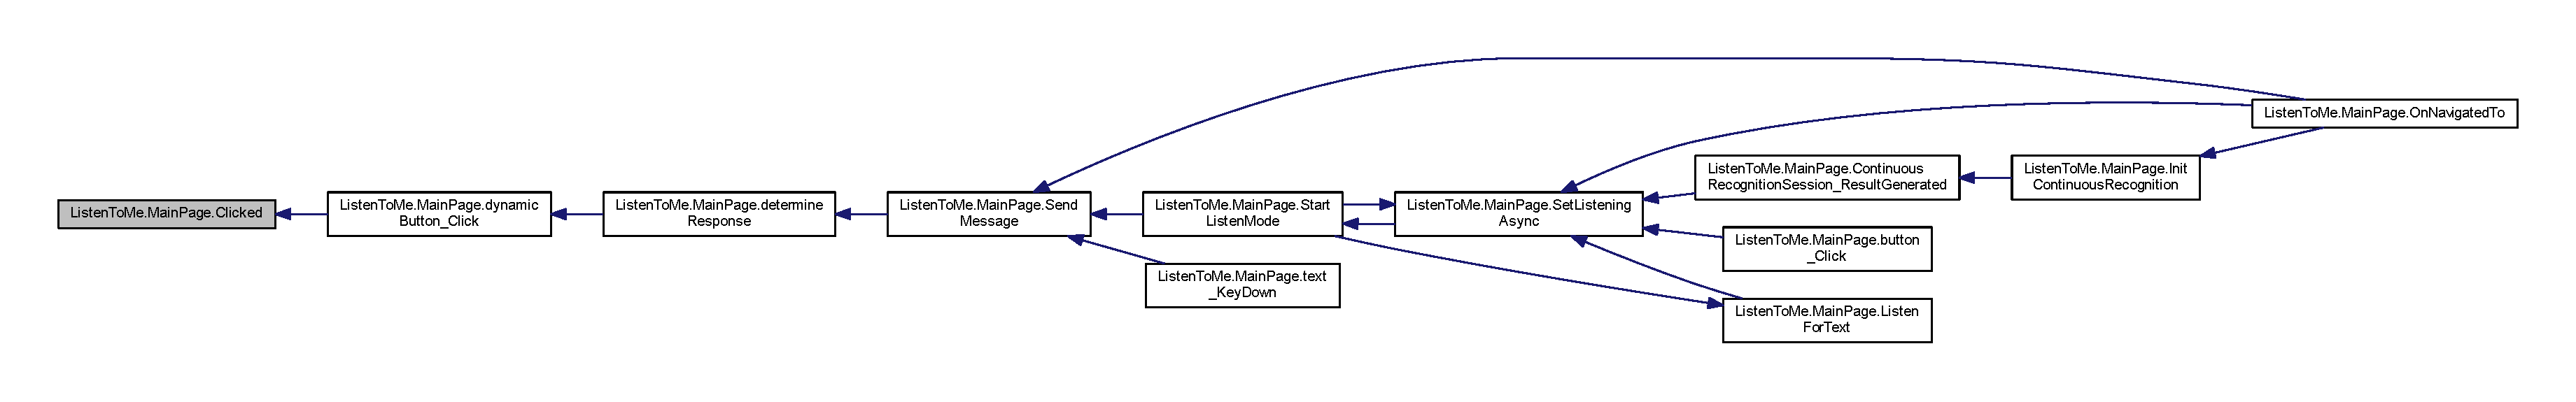
\includegraphics[width=350pt]{class_listen_to_me_1_1_main_page_a465e7f9723aec19e912a3913841d477e_icgraph}
\end{center}
\end{figure}


\index{Listen\+To\+Me\+::\+Main\+Page@{Listen\+To\+Me\+::\+Main\+Page}!Continuous\+Recognition\+Session\+\_\+\+Result\+Generated@{Continuous\+Recognition\+Session\+\_\+\+Result\+Generated}}
\index{Continuous\+Recognition\+Session\+\_\+\+Result\+Generated@{Continuous\+Recognition\+Session\+\_\+\+Result\+Generated}!Listen\+To\+Me\+::\+Main\+Page@{Listen\+To\+Me\+::\+Main\+Page}}
\subsubsection[{\texorpdfstring{Continuous\+Recognition\+Session\+\_\+\+Result\+Generated(\+Speech\+Continuous\+Recognition\+Session sender, Speech\+Continuous\+Recognition\+Result\+Generated\+Event\+Args args)}{ContinuousRecognitionSession_ResultGenerated(SpeechContinuousRecognitionSession sender, SpeechContinuousRecognitionResultGeneratedEventArgs args)}}]{\setlength{\rightskip}{0pt plus 5cm}async void Listen\+To\+Me.\+Main\+Page.\+Continuous\+Recognition\+Session\+\_\+\+Result\+Generated (
\begin{DoxyParamCaption}
\item[{Speech\+Continuous\+Recognition\+Session}]{sender, }
\item[{Speech\+Continuous\+Recognition\+Result\+Generated\+Event\+Args}]{args}
\end{DoxyParamCaption}
)\hspace{0.3cm}{\ttfamily [private]}}\hypertarget{class_listen_to_me_1_1_main_page_afad060c55f3bedc7d8e499829e133c98}{}\label{class_listen_to_me_1_1_main_page_afad060c55f3bedc7d8e499829e133c98}


Here is the call graph for this function\+:
\nopagebreak
\begin{figure}[H]
\begin{center}
\leavevmode
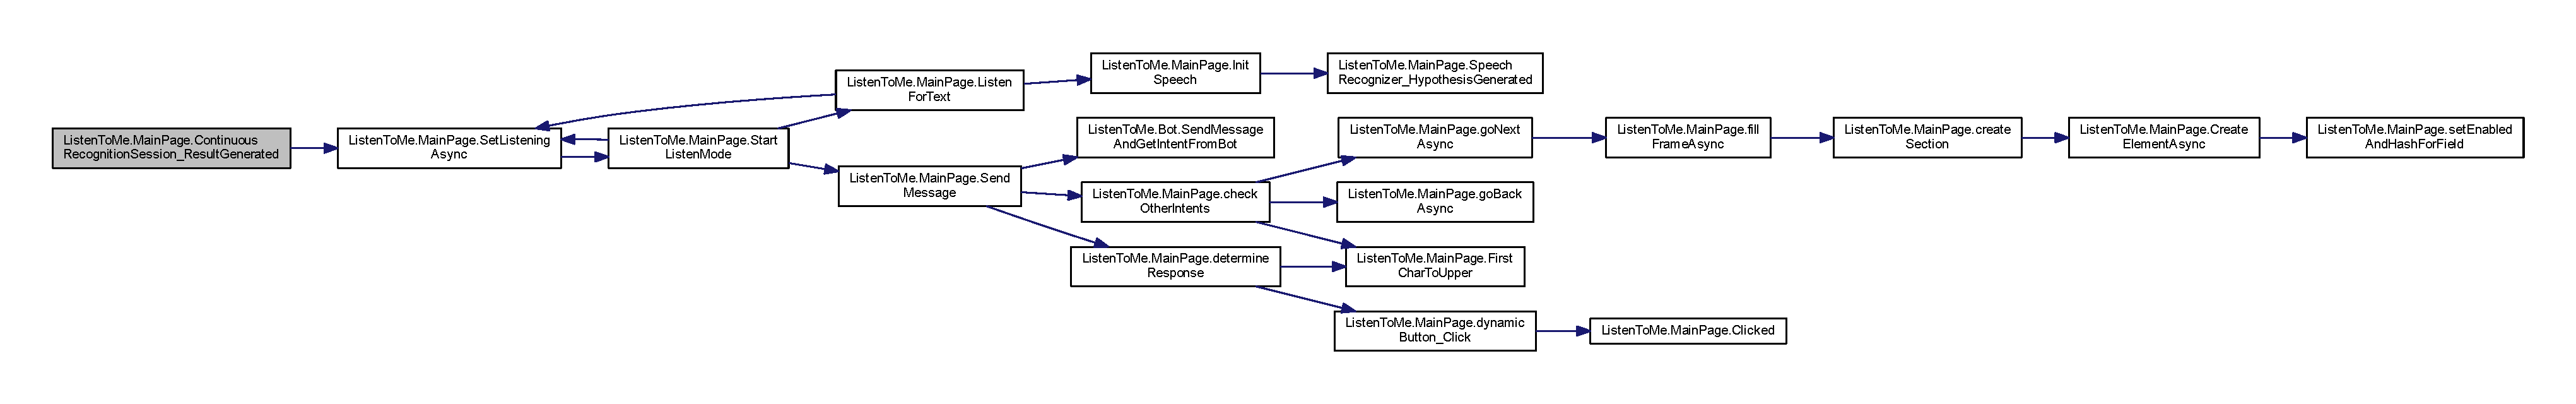
\includegraphics[width=350pt]{class_listen_to_me_1_1_main_page_afad060c55f3bedc7d8e499829e133c98_cgraph}
\end{center}
\end{figure}




Here is the caller graph for this function\+:
\nopagebreak
\begin{figure}[H]
\begin{center}
\leavevmode
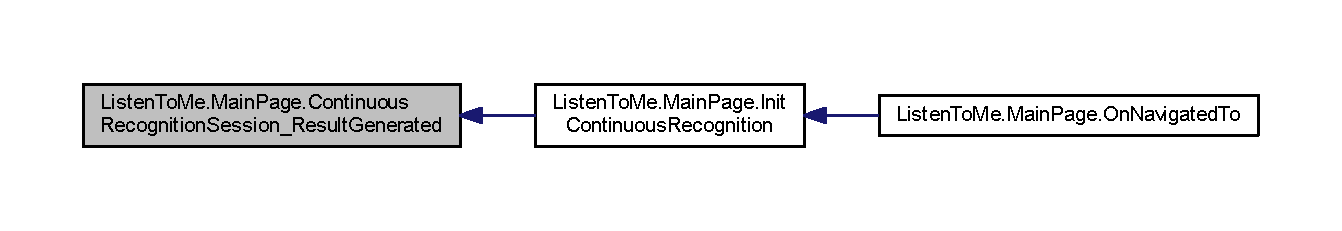
\includegraphics[width=350pt]{class_listen_to_me_1_1_main_page_afad060c55f3bedc7d8e499829e133c98_icgraph}
\end{center}
\end{figure}


\index{Listen\+To\+Me\+::\+Main\+Page@{Listen\+To\+Me\+::\+Main\+Page}!Create\+Element\+Async@{Create\+Element\+Async}}
\index{Create\+Element\+Async@{Create\+Element\+Async}!Listen\+To\+Me\+::\+Main\+Page@{Listen\+To\+Me\+::\+Main\+Page}}
\subsubsection[{\texorpdfstring{Create\+Element\+Async(\+Element element, Stack\+Panel panel, Text\+Box field=null)}{CreateElementAsync(Element element, StackPanel panel, TextBox field=null)}}]{\setlength{\rightskip}{0pt plus 5cm}async Task Listen\+To\+Me.\+Main\+Page.\+Create\+Element\+Async (
\begin{DoxyParamCaption}
\item[{Element}]{element, }
\item[{Stack\+Panel}]{panel, }
\item[{Text\+Box}]{field = {\ttfamily null}}
\end{DoxyParamCaption}
)\hspace{0.3cm}{\ttfamily [private]}}\hypertarget{class_listen_to_me_1_1_main_page_a73b3a3311149846cf028c5824dab2a6e}{}\label{class_listen_to_me_1_1_main_page_a73b3a3311149846cf028c5824dab2a6e}


creates an element from the section object by determining what type of element it is reference\+: \href{https://stackoverflow.com/questions/37297810/updatesourcetrigger-dont-work-in-wpf-customcontrols}{\tt https\+://stackoverflow.\+com/questions/37297810/updatesourcetrigger-\/dont-\/work-\/in-\/wpf-\/customcontrols} 


\begin{DoxyParams}{Parameters}
{\em element} & The element from the section\\
\hline
{\em panel} & the panel on which to add the element\\
\hline
{\em field} & as label elements have subelements, field is used for recursive calls to know the parent object\\
\hline
\end{DoxyParams}


Here is the call graph for this function\+:
\nopagebreak
\begin{figure}[H]
\begin{center}
\leavevmode
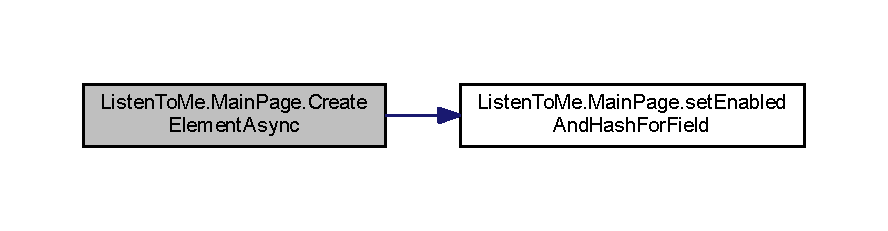
\includegraphics[width=350pt]{class_listen_to_me_1_1_main_page_a73b3a3311149846cf028c5824dab2a6e_cgraph}
\end{center}
\end{figure}




Here is the caller graph for this function\+:
\nopagebreak
\begin{figure}[H]
\begin{center}
\leavevmode
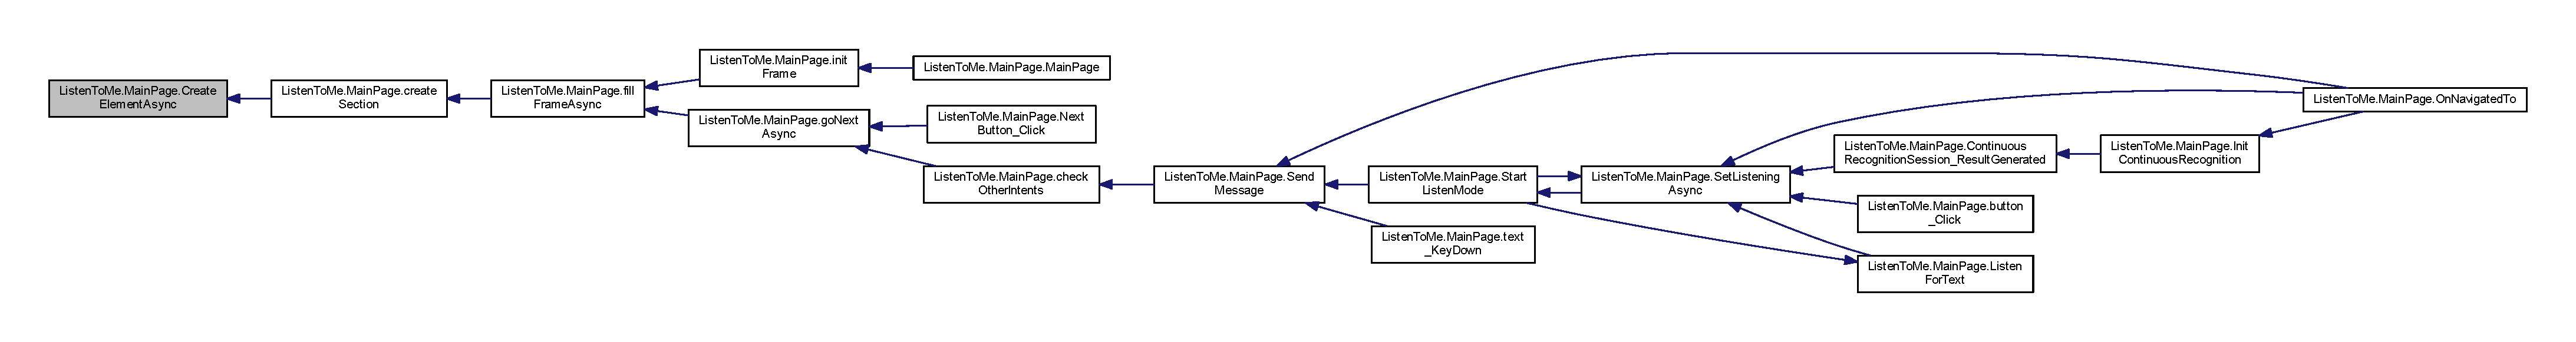
\includegraphics[width=350pt]{class_listen_to_me_1_1_main_page_a73b3a3311149846cf028c5824dab2a6e_icgraph}
\end{center}
\end{figure}


\index{Listen\+To\+Me\+::\+Main\+Page@{Listen\+To\+Me\+::\+Main\+Page}!create\+Section@{create\+Section}}
\index{create\+Section@{create\+Section}!Listen\+To\+Me\+::\+Main\+Page@{Listen\+To\+Me\+::\+Main\+Page}}
\subsubsection[{\texorpdfstring{create\+Section(\+Section section, Stack\+Panel my\+Panel)}{createSection(Section section, StackPanel myPanel)}}]{\setlength{\rightskip}{0pt plus 5cm}async Task Listen\+To\+Me.\+Main\+Page.\+create\+Section (
\begin{DoxyParamCaption}
\item[{Section}]{section, }
\item[{Stack\+Panel}]{my\+Panel}
\end{DoxyParamCaption}
)\hspace{0.3cm}{\ttfamily [private]}}\hypertarget{class_listen_to_me_1_1_main_page_a16241dfda10c37812bcb3a55a791e011}{}\label{class_listen_to_me_1_1_main_page_a16241dfda10c37812bcb3a55a791e011}


creates a section by adding control elements to a panel 


\begin{DoxyParams}{Parameters}
{\em section} & the section object that is being translated into controls\\
\hline
{\em my\+Panel} & the panel on which to place the controls\\
\hline
\end{DoxyParams}


Here is the call graph for this function\+:
\nopagebreak
\begin{figure}[H]
\begin{center}
\leavevmode
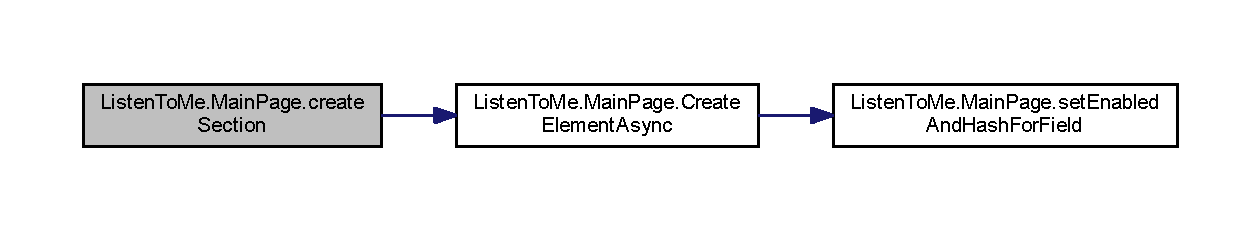
\includegraphics[width=350pt]{class_listen_to_me_1_1_main_page_a16241dfda10c37812bcb3a55a791e011_cgraph}
\end{center}
\end{figure}




Here is the caller graph for this function\+:
\nopagebreak
\begin{figure}[H]
\begin{center}
\leavevmode
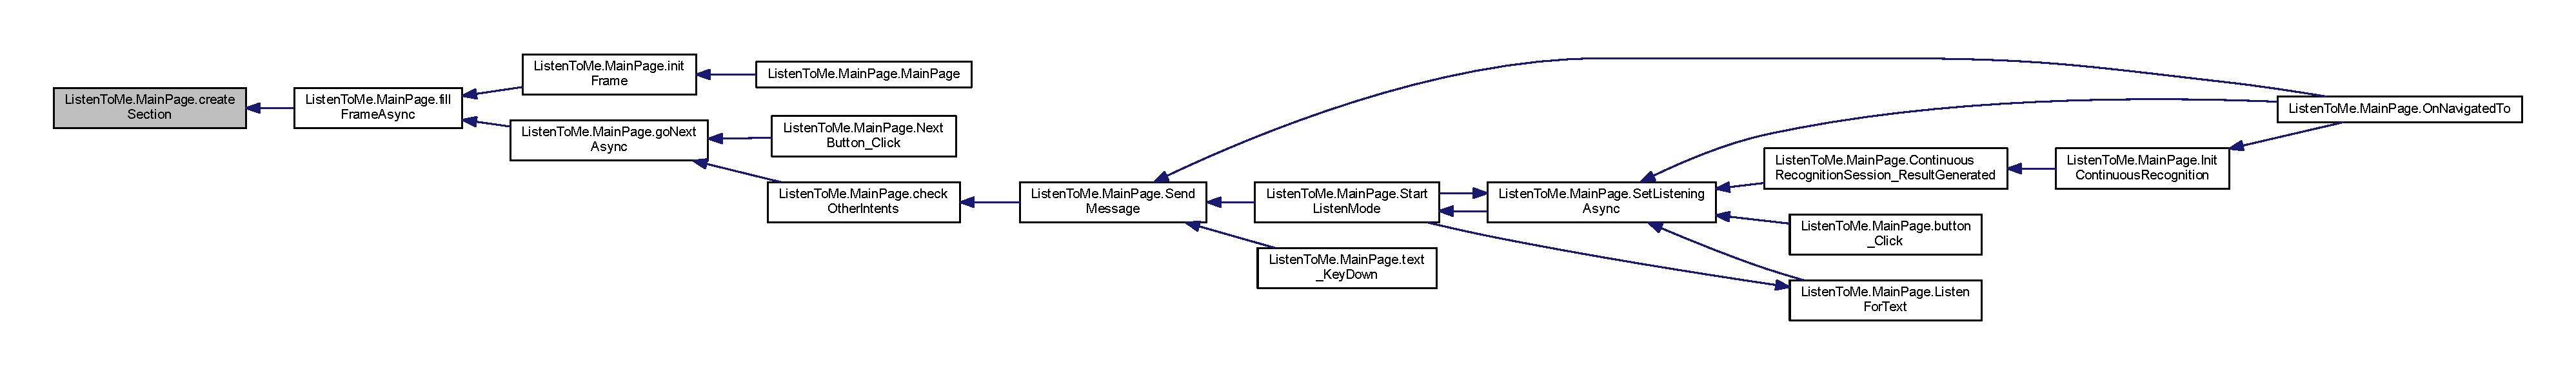
\includegraphics[width=350pt]{class_listen_to_me_1_1_main_page_a16241dfda10c37812bcb3a55a791e011_icgraph}
\end{center}
\end{figure}


\index{Listen\+To\+Me\+::\+Main\+Page@{Listen\+To\+Me\+::\+Main\+Page}!determine\+Response@{determine\+Response}}
\index{determine\+Response@{determine\+Response}!Listen\+To\+Me\+::\+Main\+Page@{Listen\+To\+Me\+::\+Main\+Page}}
\subsubsection[{\texorpdfstring{determine\+Response(string intent, string text\+Value, string users\+Field\+Name, string luis\+Type\+Of\+Text\+Value)}{determineResponse(string intent, string textValue, string usersFieldName, string luisTypeOfTextValue)}}]{\setlength{\rightskip}{0pt plus 5cm}async Task$<$string$>$ Listen\+To\+Me.\+Main\+Page.\+determine\+Response (
\begin{DoxyParamCaption}
\item[{string}]{intent, }
\item[{string}]{text\+Value, }
\item[{string}]{users\+Field\+Name, }
\item[{string}]{luis\+Type\+Of\+Text\+Value}
\end{DoxyParamCaption}
)\hspace{0.3cm}{\ttfamily [private]}}\hypertarget{class_listen_to_me_1_1_main_page_ab68e25e8370c434b0deb5069c7cdd254}{}\label{class_listen_to_me_1_1_main_page_ab68e25e8370c434b0deb5069c7cdd254}


is essential in processing the recognized L\+U\+I\+S-\/entities. Sometimes L\+U\+IS entities are not recognized by the language model. 


\begin{DoxyParams}{Parameters}
{\em intent} & the intent that L\+U\+IS recognizes. Is not importent, as this will be always Field.\+Fill\+In\\
\hline
{\em text\+Value} & the textvalue for the input field\\
\hline
{\em users\+Field\+Name} & the dirty text type name the user used in the query. \\
\hline
{\em luis\+Type\+Of\+Text\+Value} & the clean text type\\
\hline
\end{DoxyParams}
\begin{DoxyReturn}{Returns}
error messages
\end{DoxyReturn}


Here is the call graph for this function\+:
\nopagebreak
\begin{figure}[H]
\begin{center}
\leavevmode
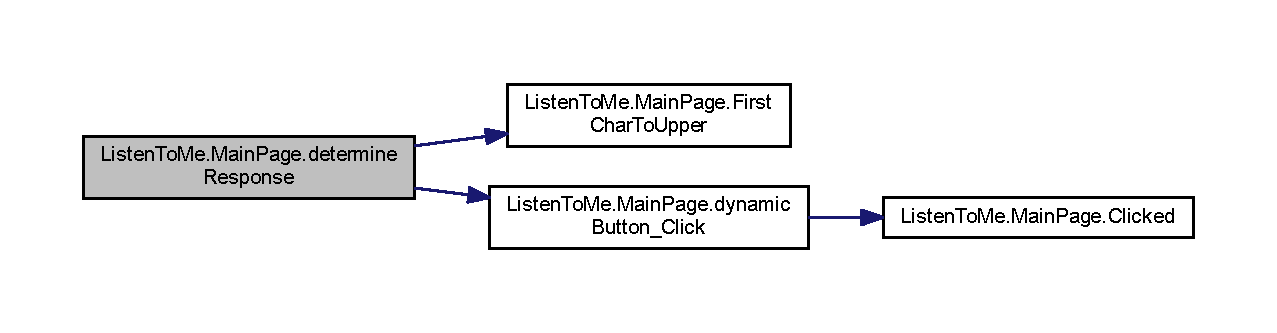
\includegraphics[width=350pt]{class_listen_to_me_1_1_main_page_ab68e25e8370c434b0deb5069c7cdd254_cgraph}
\end{center}
\end{figure}




Here is the caller graph for this function\+:
\nopagebreak
\begin{figure}[H]
\begin{center}
\leavevmode
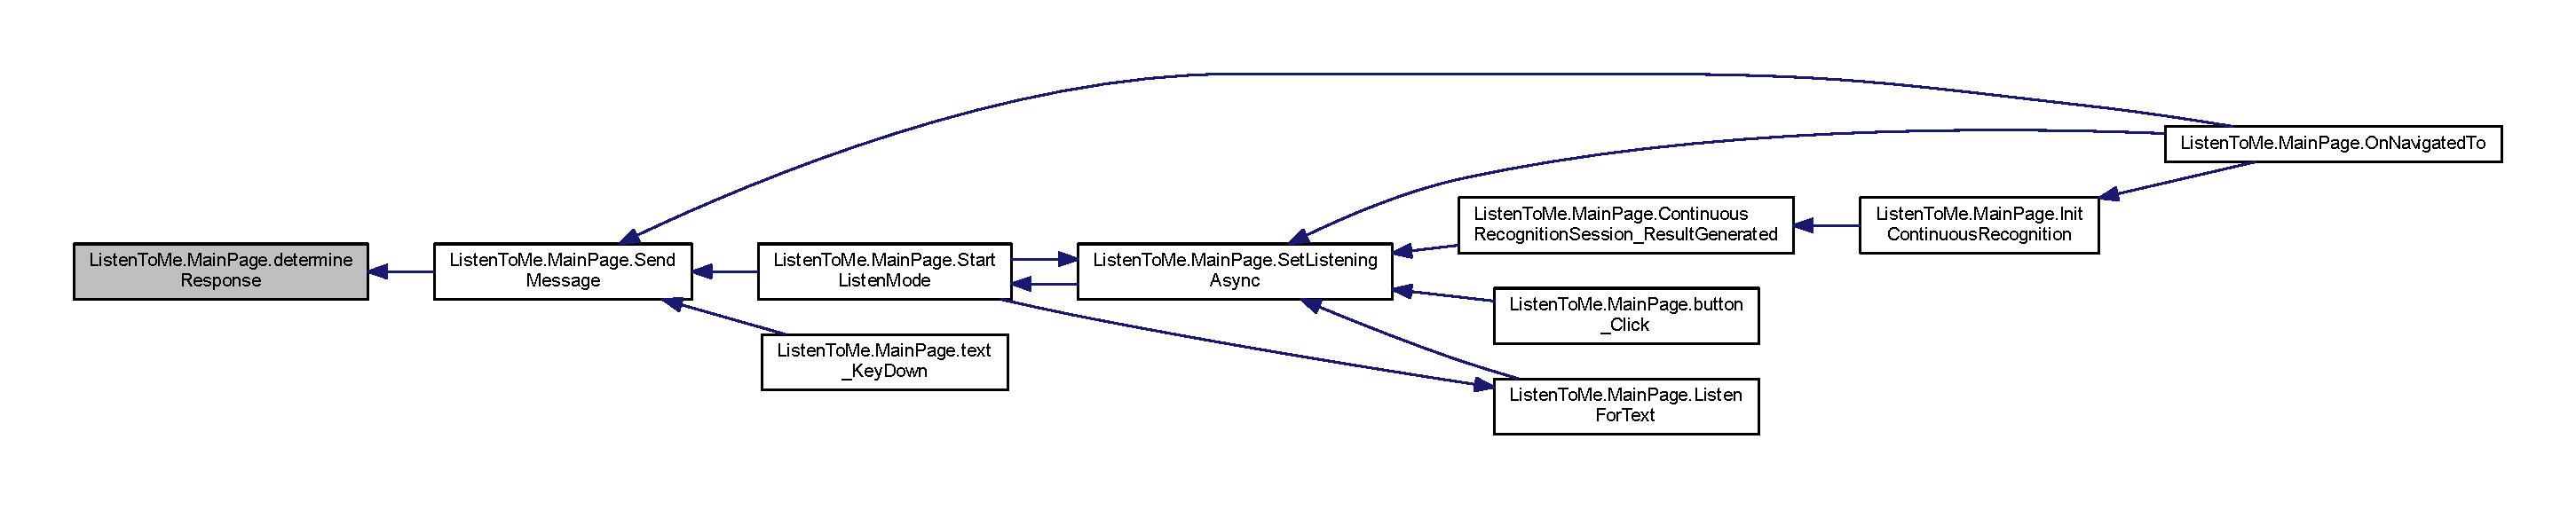
\includegraphics[width=350pt]{class_listen_to_me_1_1_main_page_ab68e25e8370c434b0deb5069c7cdd254_icgraph}
\end{center}
\end{figure}


\index{Listen\+To\+Me\+::\+Main\+Page@{Listen\+To\+Me\+::\+Main\+Page}!dynamic\+Button\+\_\+\+Click@{dynamic\+Button\+\_\+\+Click}}
\index{dynamic\+Button\+\_\+\+Click@{dynamic\+Button\+\_\+\+Click}!Listen\+To\+Me\+::\+Main\+Page@{Listen\+To\+Me\+::\+Main\+Page}}
\subsubsection[{\texorpdfstring{dynamic\+Button\+\_\+\+Click(object sender, Routed\+Event\+Args e)}{dynamicButton_Click(object sender, RoutedEventArgs e)}}]{\setlength{\rightskip}{0pt plus 5cm}void Listen\+To\+Me.\+Main\+Page.\+dynamic\+Button\+\_\+\+Click (
\begin{DoxyParamCaption}
\item[{object}]{sender, }
\item[{Routed\+Event\+Args}]{e}
\end{DoxyParamCaption}
)\hspace{0.3cm}{\ttfamily [private]}}\hypertarget{class_listen_to_me_1_1_main_page_acad3fb1a64c0bea077f5ad38627faeef}{}\label{class_listen_to_me_1_1_main_page_acad3fb1a64c0bea077f5ad38627faeef}


Button is hit for microphone activation 


\begin{DoxyParams}{Parameters}
{\em sender} & the microphone button\\
\hline
{\em e} & some eventarguments\\
\hline
\end{DoxyParams}


Here is the call graph for this function\+:
\nopagebreak
\begin{figure}[H]
\begin{center}
\leavevmode
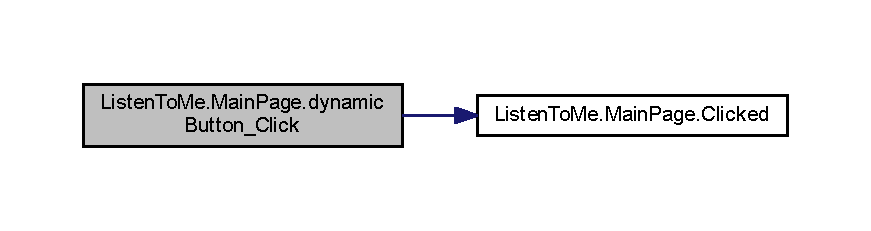
\includegraphics[width=350pt]{class_listen_to_me_1_1_main_page_acad3fb1a64c0bea077f5ad38627faeef_cgraph}
\end{center}
\end{figure}




Here is the caller graph for this function\+:
\nopagebreak
\begin{figure}[H]
\begin{center}
\leavevmode
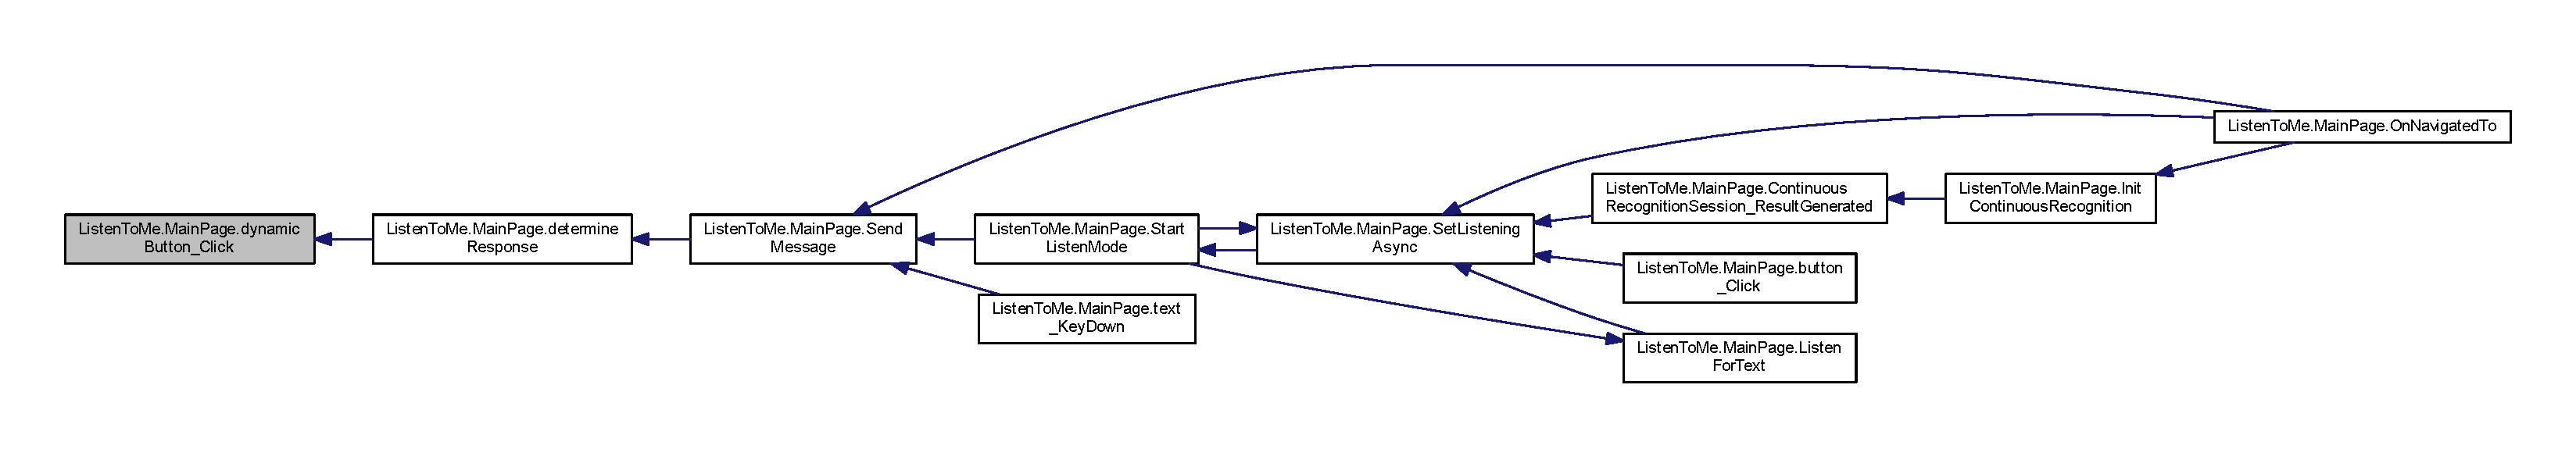
\includegraphics[width=350pt]{class_listen_to_me_1_1_main_page_acad3fb1a64c0bea077f5ad38627faeef_icgraph}
\end{center}
\end{figure}


\index{Listen\+To\+Me\+::\+Main\+Page@{Listen\+To\+Me\+::\+Main\+Page}!fill\+Frame\+Async@{fill\+Frame\+Async}}
\index{fill\+Frame\+Async@{fill\+Frame\+Async}!Listen\+To\+Me\+::\+Main\+Page@{Listen\+To\+Me\+::\+Main\+Page}}
\subsubsection[{\texorpdfstring{fill\+Frame\+Async()}{fillFrameAsync()}}]{\setlength{\rightskip}{0pt plus 5cm}async Task Listen\+To\+Me.\+Main\+Page.\+fill\+Frame\+Async (
\begin{DoxyParamCaption}
{}
\end{DoxyParamCaption}
)\hspace{0.3cm}{\ttfamily [private]}}\hypertarget{class_listen_to_me_1_1_main_page_a1a1e1d6e362134f6426bcf99ca83c45c}{}\label{class_listen_to_me_1_1_main_page_a1a1e1d6e362134f6426bcf99ca83c45c}


fill Frame creates a new Page for main\+Frame and adds it to the main\+Frame as Content 


\begin{DoxyParams}{Parameters}
{\em rnd} & random element signalling background Page\textquotesingle{}s colour\\
\hline
\end{DoxyParams}


Here is the call graph for this function\+:
\nopagebreak
\begin{figure}[H]
\begin{center}
\leavevmode
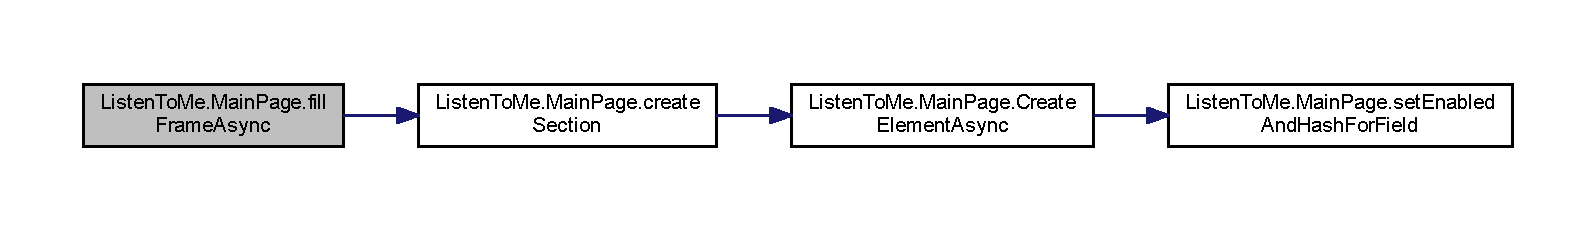
\includegraphics[width=350pt]{class_listen_to_me_1_1_main_page_a1a1e1d6e362134f6426bcf99ca83c45c_cgraph}
\end{center}
\end{figure}




Here is the caller graph for this function\+:
\nopagebreak
\begin{figure}[H]
\begin{center}
\leavevmode
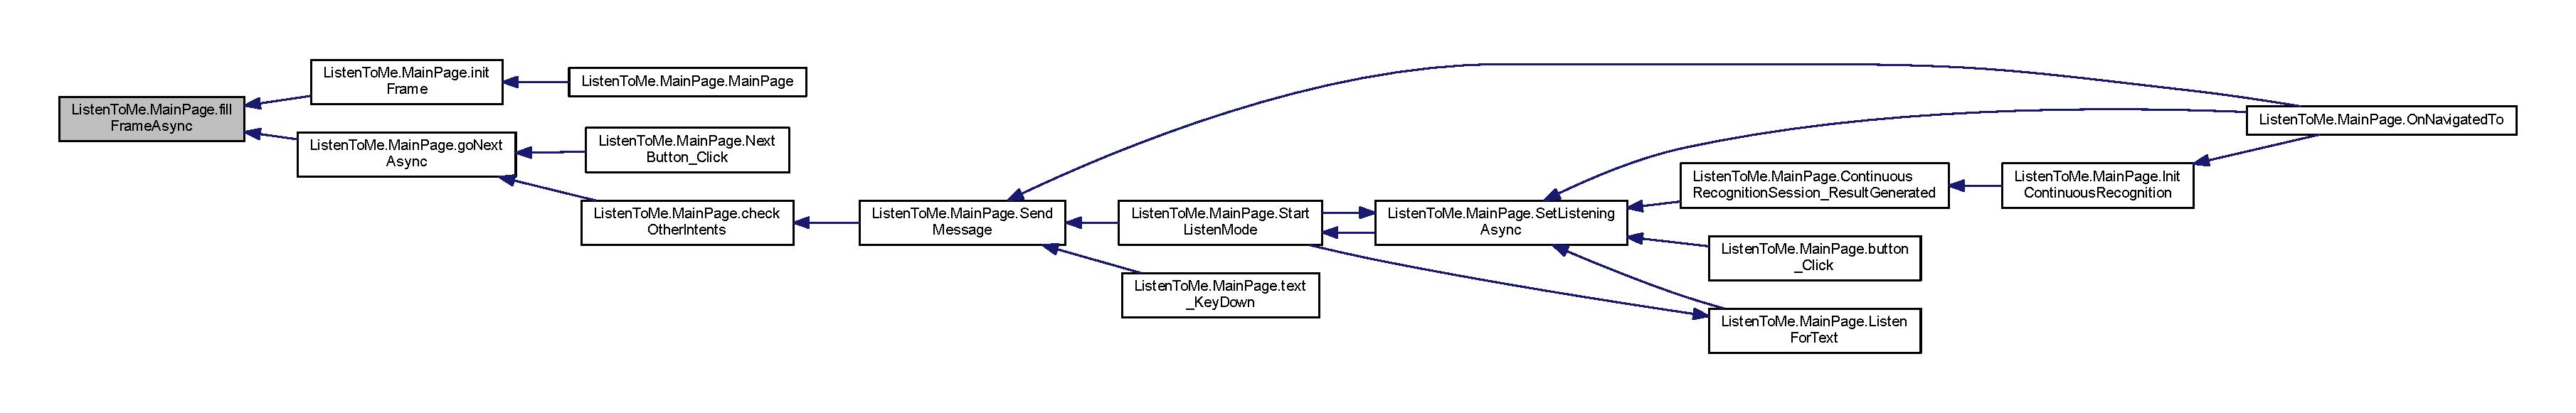
\includegraphics[width=350pt]{class_listen_to_me_1_1_main_page_a1a1e1d6e362134f6426bcf99ca83c45c_icgraph}
\end{center}
\end{figure}


\index{Listen\+To\+Me\+::\+Main\+Page@{Listen\+To\+Me\+::\+Main\+Page}!First\+Char\+To\+Upper@{First\+Char\+To\+Upper}}
\index{First\+Char\+To\+Upper@{First\+Char\+To\+Upper}!Listen\+To\+Me\+::\+Main\+Page@{Listen\+To\+Me\+::\+Main\+Page}}
\subsubsection[{\texorpdfstring{First\+Char\+To\+Upper(string input)}{FirstCharToUpper(string input)}}]{\setlength{\rightskip}{0pt plus 5cm}static string Listen\+To\+Me.\+Main\+Page.\+First\+Char\+To\+Upper (
\begin{DoxyParamCaption}
\item[{string}]{input}
\end{DoxyParamCaption}
)\hspace{0.3cm}{\ttfamily [static]}}\hypertarget{class_listen_to_me_1_1_main_page_af4469348ffee9a5d1a8680d2535a279b}{}\label{class_listen_to_me_1_1_main_page_af4469348ffee9a5d1a8680d2535a279b}


helper method for cleaning output from luis. Since L\+U\+IS answers in lowercase only, this method uppercases the first letter 


\begin{DoxyParams}{Parameters}
{\em input} & \\
\hline
\end{DoxyParams}
\begin{DoxyReturn}{Returns}

\end{DoxyReturn}


Here is the caller graph for this function\+:
\nopagebreak
\begin{figure}[H]
\begin{center}
\leavevmode
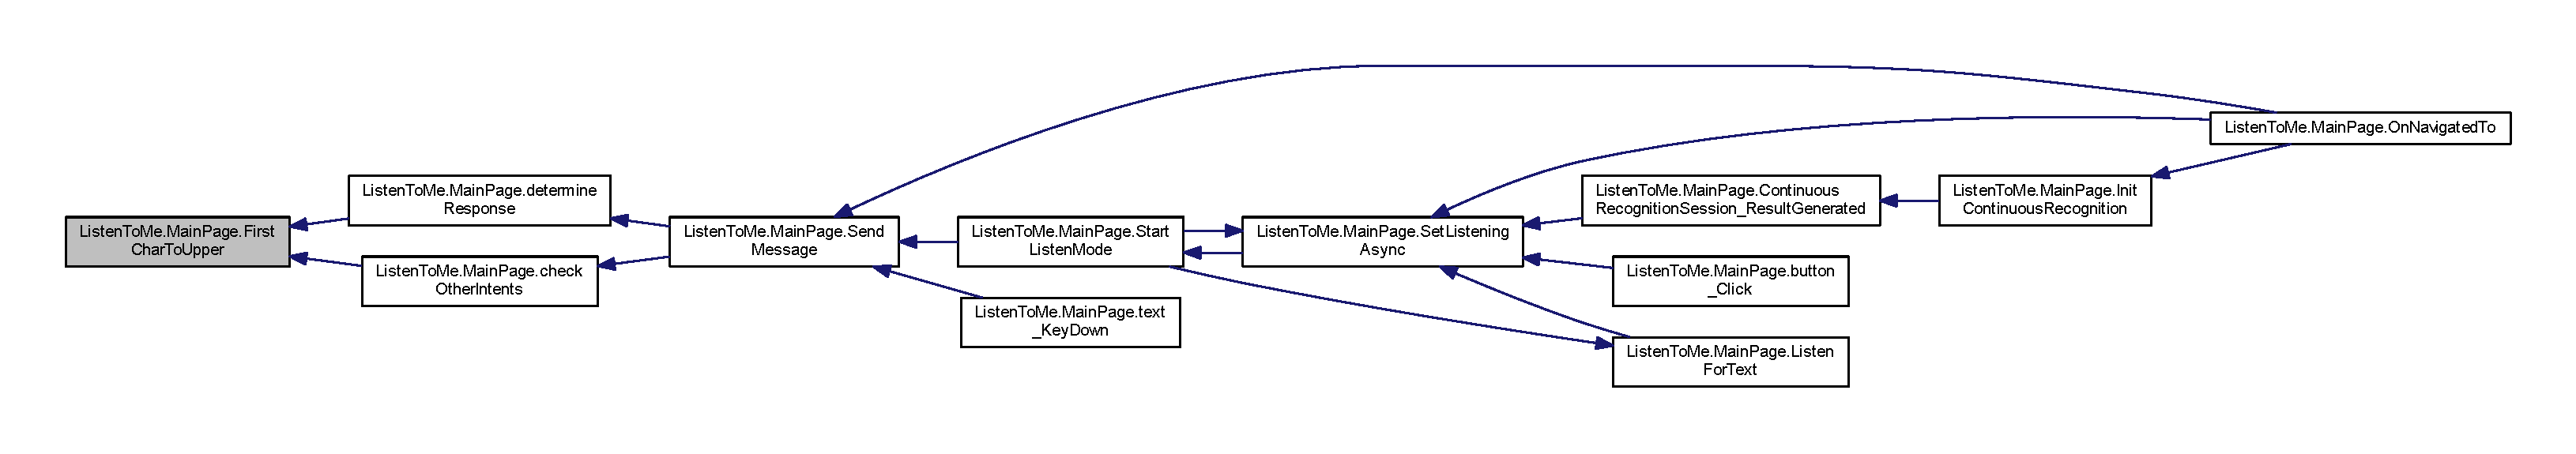
\includegraphics[width=350pt]{class_listen_to_me_1_1_main_page_af4469348ffee9a5d1a8680d2535a279b_icgraph}
\end{center}
\end{figure}


\index{Listen\+To\+Me\+::\+Main\+Page@{Listen\+To\+Me\+::\+Main\+Page}!go\+Back\+Async@{go\+Back\+Async}}
\index{go\+Back\+Async@{go\+Back\+Async}!Listen\+To\+Me\+::\+Main\+Page@{Listen\+To\+Me\+::\+Main\+Page}}
\subsubsection[{\texorpdfstring{go\+Back\+Async()}{goBackAsync()}}]{\setlength{\rightskip}{0pt plus 5cm}async Task Listen\+To\+Me.\+Main\+Page.\+go\+Back\+Async (
\begin{DoxyParamCaption}
{}
\end{DoxyParamCaption}
)\hspace{0.3cm}{\ttfamily [private]}}\hypertarget{class_listen_to_me_1_1_main_page_a1ccf14d59eabbcc4148cadd8dd11fc04}{}\label{class_listen_to_me_1_1_main_page_a1ccf14d59eabbcc4148cadd8dd11fc04}


Here is the caller graph for this function\+:
\nopagebreak
\begin{figure}[H]
\begin{center}
\leavevmode
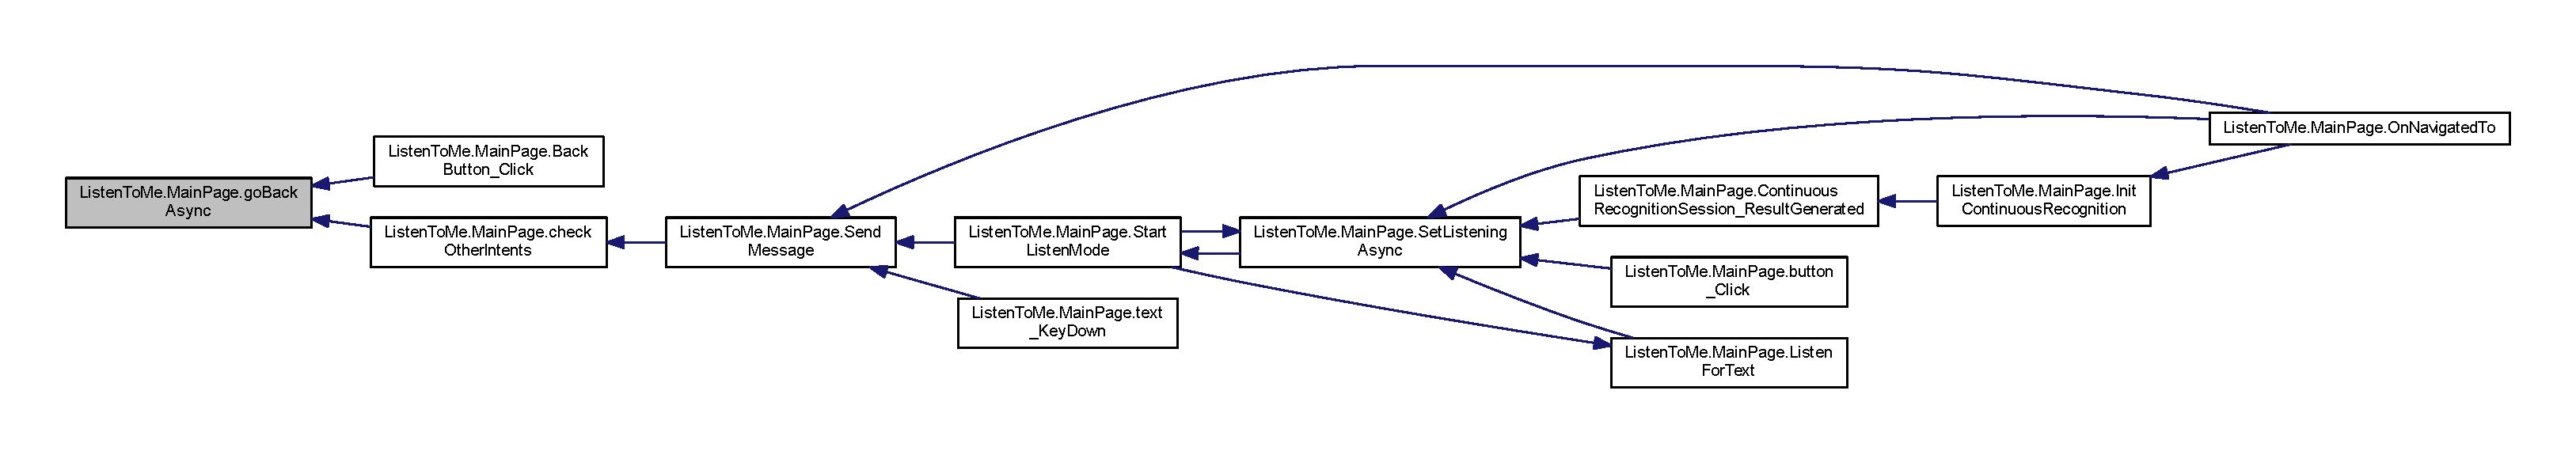
\includegraphics[width=350pt]{class_listen_to_me_1_1_main_page_a1ccf14d59eabbcc4148cadd8dd11fc04_icgraph}
\end{center}
\end{figure}


\index{Listen\+To\+Me\+::\+Main\+Page@{Listen\+To\+Me\+::\+Main\+Page}!go\+Next\+Async@{go\+Next\+Async}}
\index{go\+Next\+Async@{go\+Next\+Async}!Listen\+To\+Me\+::\+Main\+Page@{Listen\+To\+Me\+::\+Main\+Page}}
\subsubsection[{\texorpdfstring{go\+Next\+Async()}{goNextAsync()}}]{\setlength{\rightskip}{0pt plus 5cm}async Task Listen\+To\+Me.\+Main\+Page.\+go\+Next\+Async (
\begin{DoxyParamCaption}
{}
\end{DoxyParamCaption}
)\hspace{0.3cm}{\ttfamily [private]}}\hypertarget{class_listen_to_me_1_1_main_page_a8cd1a04a404800cfab55de0ba4466f68}{}\label{class_listen_to_me_1_1_main_page_a8cd1a04a404800cfab55de0ba4466f68}


Here is the call graph for this function\+:
\nopagebreak
\begin{figure}[H]
\begin{center}
\leavevmode
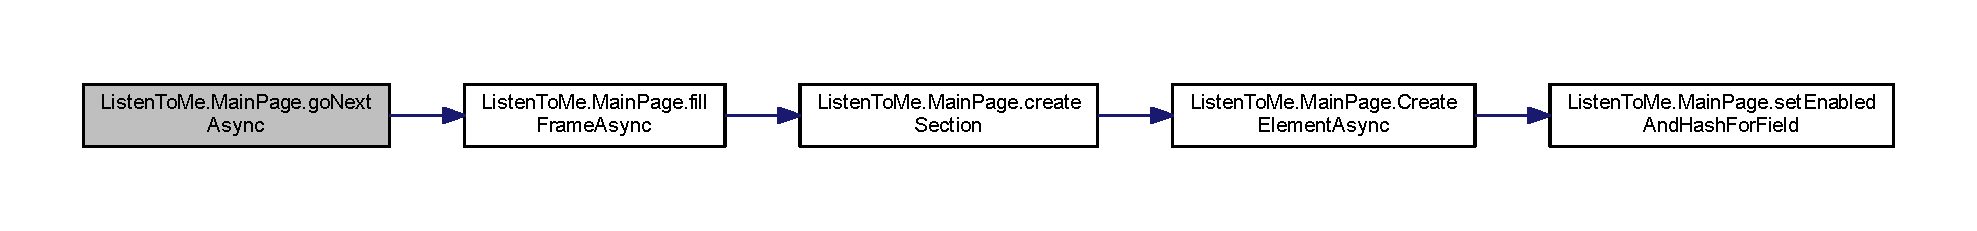
\includegraphics[width=350pt]{class_listen_to_me_1_1_main_page_a8cd1a04a404800cfab55de0ba4466f68_cgraph}
\end{center}
\end{figure}




Here is the caller graph for this function\+:
\nopagebreak
\begin{figure}[H]
\begin{center}
\leavevmode
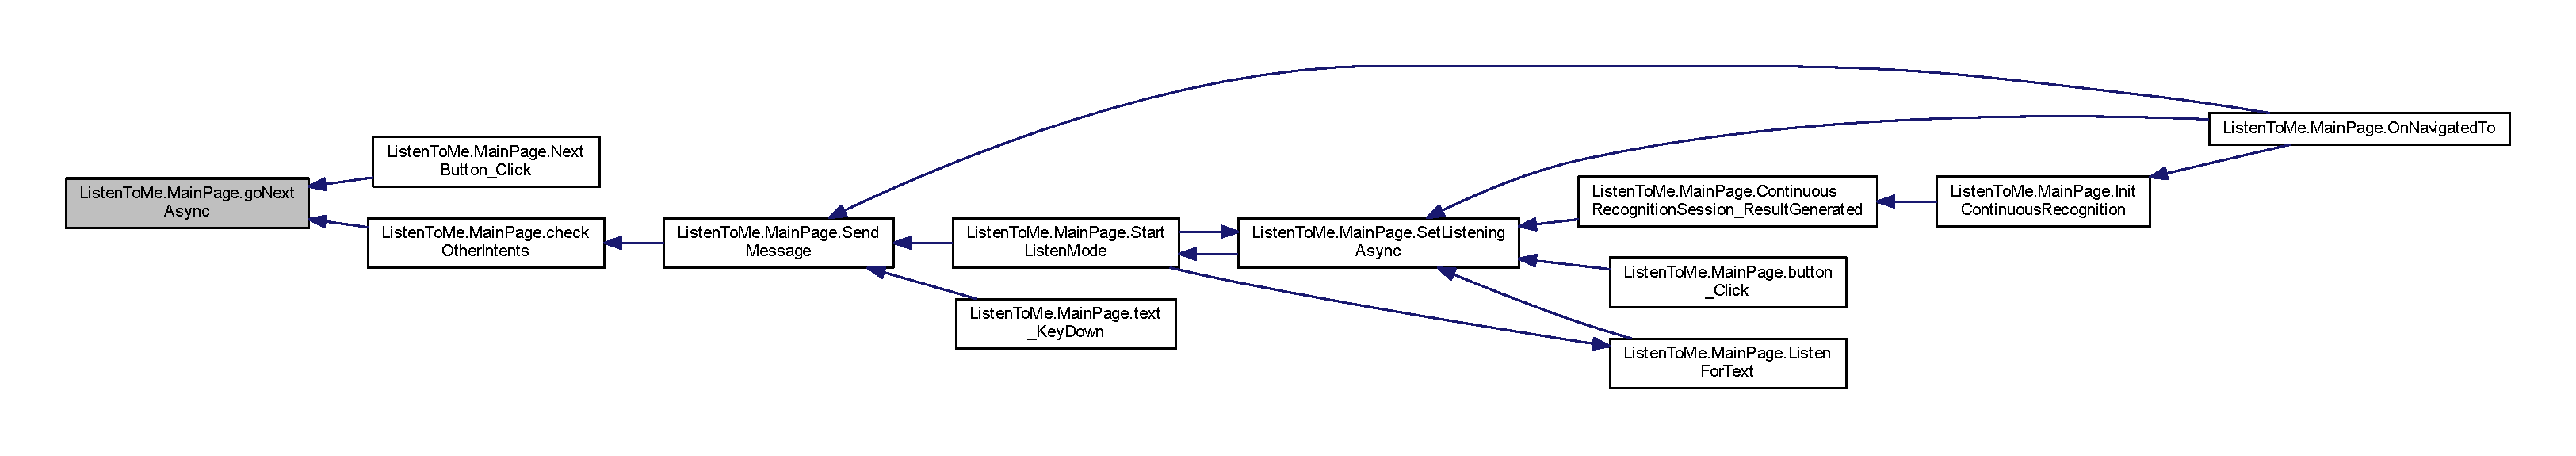
\includegraphics[width=350pt]{class_listen_to_me_1_1_main_page_a8cd1a04a404800cfab55de0ba4466f68_icgraph}
\end{center}
\end{figure}


\index{Listen\+To\+Me\+::\+Main\+Page@{Listen\+To\+Me\+::\+Main\+Page}!Home\+Button\+\_\+\+Click@{Home\+Button\+\_\+\+Click}}
\index{Home\+Button\+\_\+\+Click@{Home\+Button\+\_\+\+Click}!Listen\+To\+Me\+::\+Main\+Page@{Listen\+To\+Me\+::\+Main\+Page}}
\subsubsection[{\texorpdfstring{Home\+Button\+\_\+\+Click(object sender, Routed\+Event\+Args e)}{HomeButton_Click(object sender, RoutedEventArgs e)}}]{\setlength{\rightskip}{0pt plus 5cm}async void Listen\+To\+Me.\+Main\+Page.\+Home\+Button\+\_\+\+Click (
\begin{DoxyParamCaption}
\item[{object}]{sender, }
\item[{Routed\+Event\+Args}]{e}
\end{DoxyParamCaption}
)\hspace{0.3cm}{\ttfamily [private]}}\hypertarget{class_listen_to_me_1_1_main_page_a4dec5880c4a900edea6e9a2f37cd93fc}{}\label{class_listen_to_me_1_1_main_page_a4dec5880c4a900edea6e9a2f37cd93fc}


has no speacial meaning as of yet 


\begin{DoxyParams}{Parameters}
{\em sender} & \\
\hline
{\em e} & \\
\hline
\end{DoxyParams}
\index{Listen\+To\+Me\+::\+Main\+Page@{Listen\+To\+Me\+::\+Main\+Page}!Init\+Continuous\+Recognition@{Init\+Continuous\+Recognition}}
\index{Init\+Continuous\+Recognition@{Init\+Continuous\+Recognition}!Listen\+To\+Me\+::\+Main\+Page@{Listen\+To\+Me\+::\+Main\+Page}}
\subsubsection[{\texorpdfstring{Init\+Continuous\+Recognition()}{InitContinuousRecognition()}}]{\setlength{\rightskip}{0pt plus 5cm}async Task Listen\+To\+Me.\+Main\+Page.\+Init\+Continuous\+Recognition (
\begin{DoxyParamCaption}
{}
\end{DoxyParamCaption}
)\hspace{0.3cm}{\ttfamily [private]}}\hypertarget{class_listen_to_me_1_1_main_page_adbf1a6a0cab368d6e803bbd1b918a045}{}\label{class_listen_to_me_1_1_main_page_adbf1a6a0cab368d6e803bbd1b918a045}


sets up continous speech recognition 

\begin{DoxyReturn}{Returns}

\end{DoxyReturn}


Here is the call graph for this function\+:
\nopagebreak
\begin{figure}[H]
\begin{center}
\leavevmode
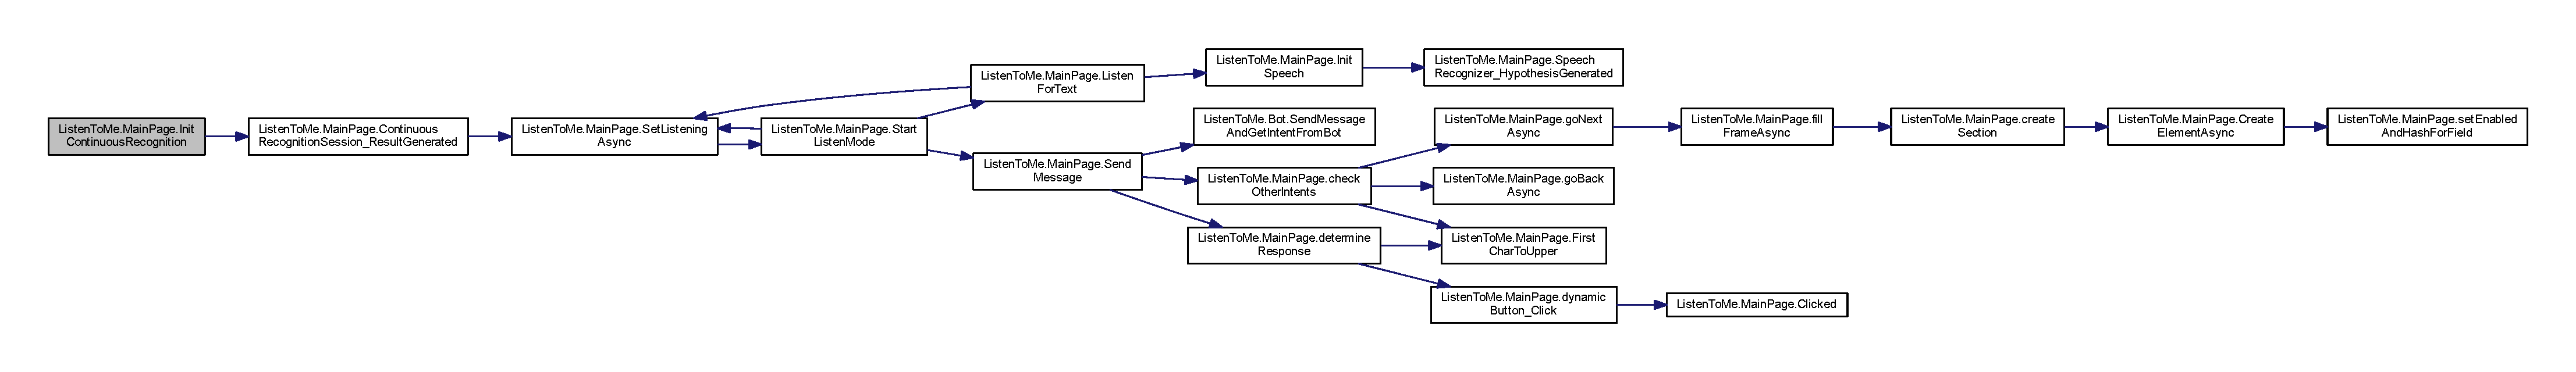
\includegraphics[width=350pt]{class_listen_to_me_1_1_main_page_adbf1a6a0cab368d6e803bbd1b918a045_cgraph}
\end{center}
\end{figure}




Here is the caller graph for this function\+:
\nopagebreak
\begin{figure}[H]
\begin{center}
\leavevmode
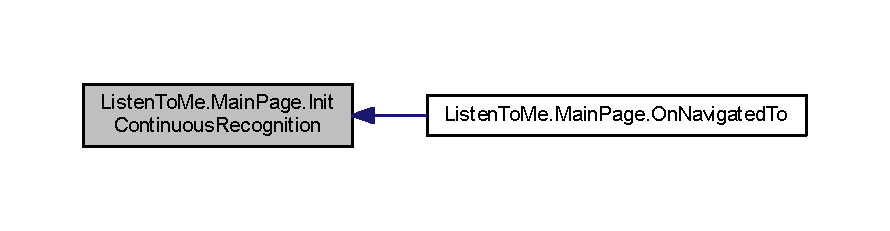
\includegraphics[width=350pt]{class_listen_to_me_1_1_main_page_adbf1a6a0cab368d6e803bbd1b918a045_icgraph}
\end{center}
\end{figure}


\index{Listen\+To\+Me\+::\+Main\+Page@{Listen\+To\+Me\+::\+Main\+Page}!init\+Frame@{init\+Frame}}
\index{init\+Frame@{init\+Frame}!Listen\+To\+Me\+::\+Main\+Page@{Listen\+To\+Me\+::\+Main\+Page}}
\subsubsection[{\texorpdfstring{init\+Frame()}{initFrame()}}]{\setlength{\rightskip}{0pt plus 5cm}async void Listen\+To\+Me.\+Main\+Page.\+init\+Frame (
\begin{DoxyParamCaption}
{}
\end{DoxyParamCaption}
)\hspace{0.3cm}{\ttfamily [private]}}\hypertarget{class_listen_to_me_1_1_main_page_a781bed1ae1145079c62597b5a938c0d1}{}\label{class_listen_to_me_1_1_main_page_a781bed1ae1145079c62597b5a938c0d1}


fills the section field in formstore with information from the web form 



Here is the call graph for this function\+:
\nopagebreak
\begin{figure}[H]
\begin{center}
\leavevmode
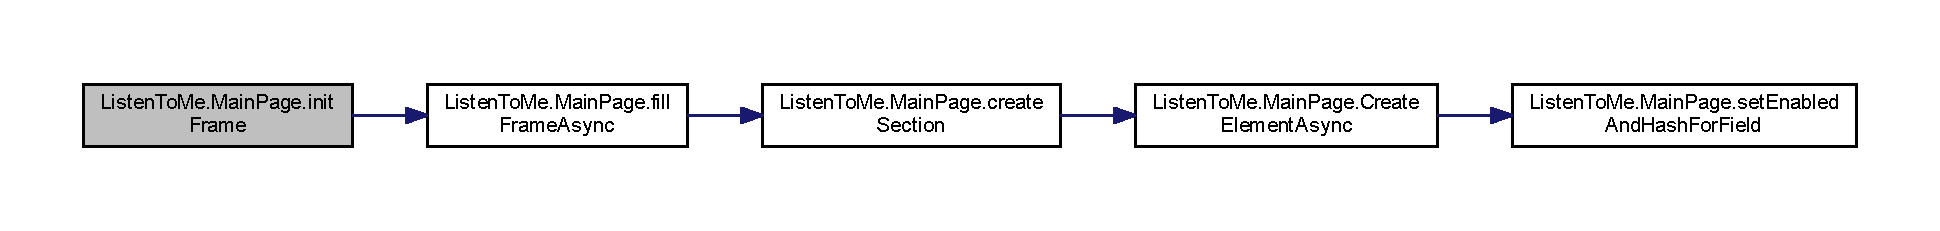
\includegraphics[width=350pt]{class_listen_to_me_1_1_main_page_a781bed1ae1145079c62597b5a938c0d1_cgraph}
\end{center}
\end{figure}




Here is the caller graph for this function\+:
\nopagebreak
\begin{figure}[H]
\begin{center}
\leavevmode
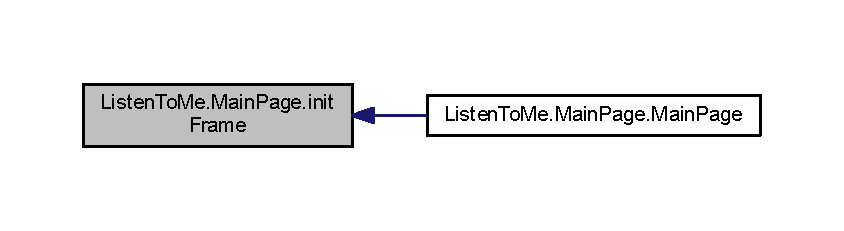
\includegraphics[width=350pt]{class_listen_to_me_1_1_main_page_a781bed1ae1145079c62597b5a938c0d1_icgraph}
\end{center}
\end{figure}


\index{Listen\+To\+Me\+::\+Main\+Page@{Listen\+To\+Me\+::\+Main\+Page}!Init\+Speech@{Init\+Speech}}
\index{Init\+Speech@{Init\+Speech}!Listen\+To\+Me\+::\+Main\+Page@{Listen\+To\+Me\+::\+Main\+Page}}
\subsubsection[{\texorpdfstring{Init\+Speech()}{InitSpeech()}}]{\setlength{\rightskip}{0pt plus 5cm}async Task Listen\+To\+Me.\+Main\+Page.\+Init\+Speech (
\begin{DoxyParamCaption}
{}
\end{DoxyParamCaption}
)\hspace{0.3cm}{\ttfamily [private]}}\hypertarget{class_listen_to_me_1_1_main_page_ac541bec23372af9da39117384c6b177e}{}\label{class_listen_to_me_1_1_main_page_ac541bec23372af9da39117384c6b177e}


initialized speech recognition 



Here is the call graph for this function\+:
\nopagebreak
\begin{figure}[H]
\begin{center}
\leavevmode
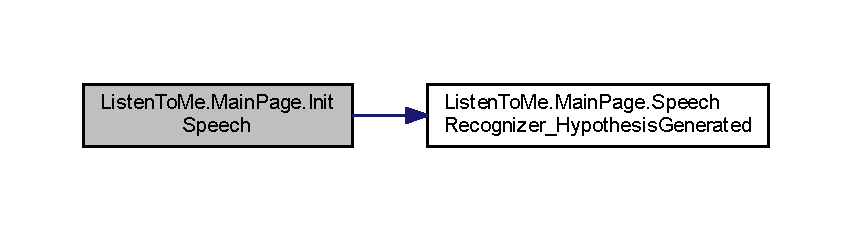
\includegraphics[width=350pt]{class_listen_to_me_1_1_main_page_ac541bec23372af9da39117384c6b177e_cgraph}
\end{center}
\end{figure}




Here is the caller graph for this function\+:
\nopagebreak
\begin{figure}[H]
\begin{center}
\leavevmode
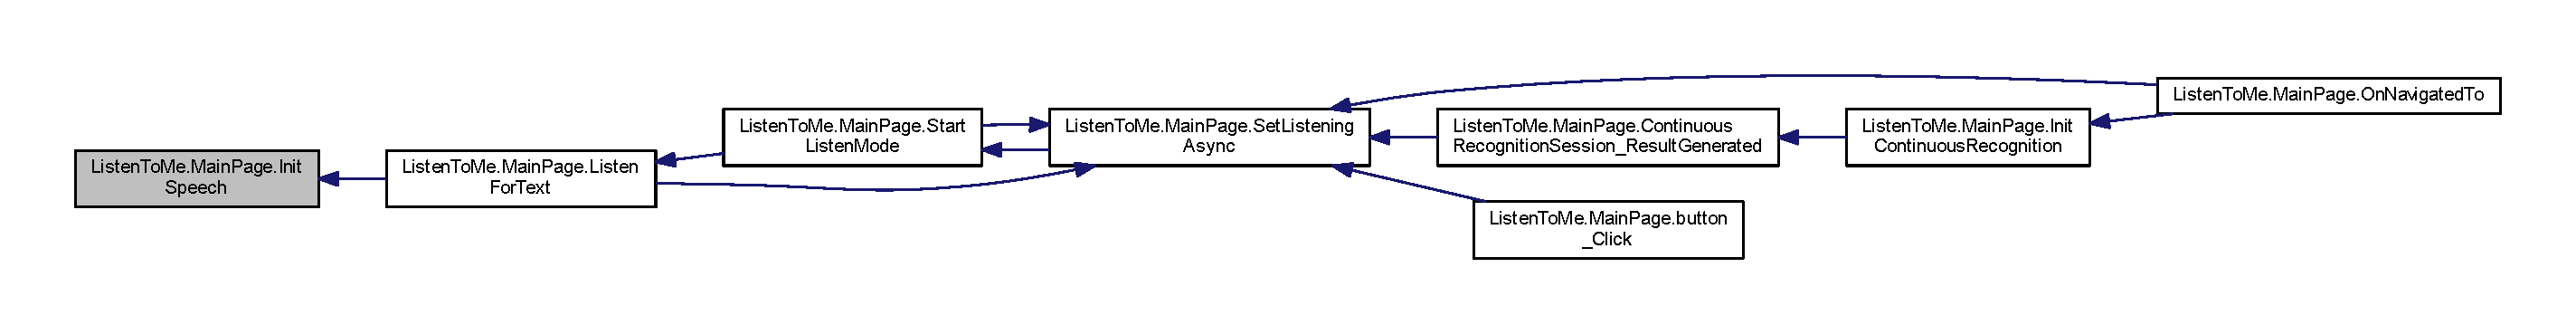
\includegraphics[width=350pt]{class_listen_to_me_1_1_main_page_ac541bec23372af9da39117384c6b177e_icgraph}
\end{center}
\end{figure}


\index{Listen\+To\+Me\+::\+Main\+Page@{Listen\+To\+Me\+::\+Main\+Page}!Listen\+For\+Text@{Listen\+For\+Text}}
\index{Listen\+For\+Text@{Listen\+For\+Text}!Listen\+To\+Me\+::\+Main\+Page@{Listen\+To\+Me\+::\+Main\+Page}}
\subsubsection[{\texorpdfstring{Listen\+For\+Text()}{ListenForText()}}]{\setlength{\rightskip}{0pt plus 5cm}async Task$<$string$>$ Listen\+To\+Me.\+Main\+Page.\+Listen\+For\+Text (
\begin{DoxyParamCaption}
{}
\end{DoxyParamCaption}
)\hspace{0.3cm}{\ttfamily [private]}}\hypertarget{class_listen_to_me_1_1_main_page_a94a7dfd5dc1ec2e9bf7a86a4b9f7df0c}{}\label{class_listen_to_me_1_1_main_page_a94a7dfd5dc1ec2e9bf7a86a4b9f7df0c}


handles exceptions in the speechrecognition api. Also checks whether the device the user in using has enabled microphone input 

\begin{DoxyReturn}{Returns}

\end{DoxyReturn}


Here is the call graph for this function\+:
\nopagebreak
\begin{figure}[H]
\begin{center}
\leavevmode
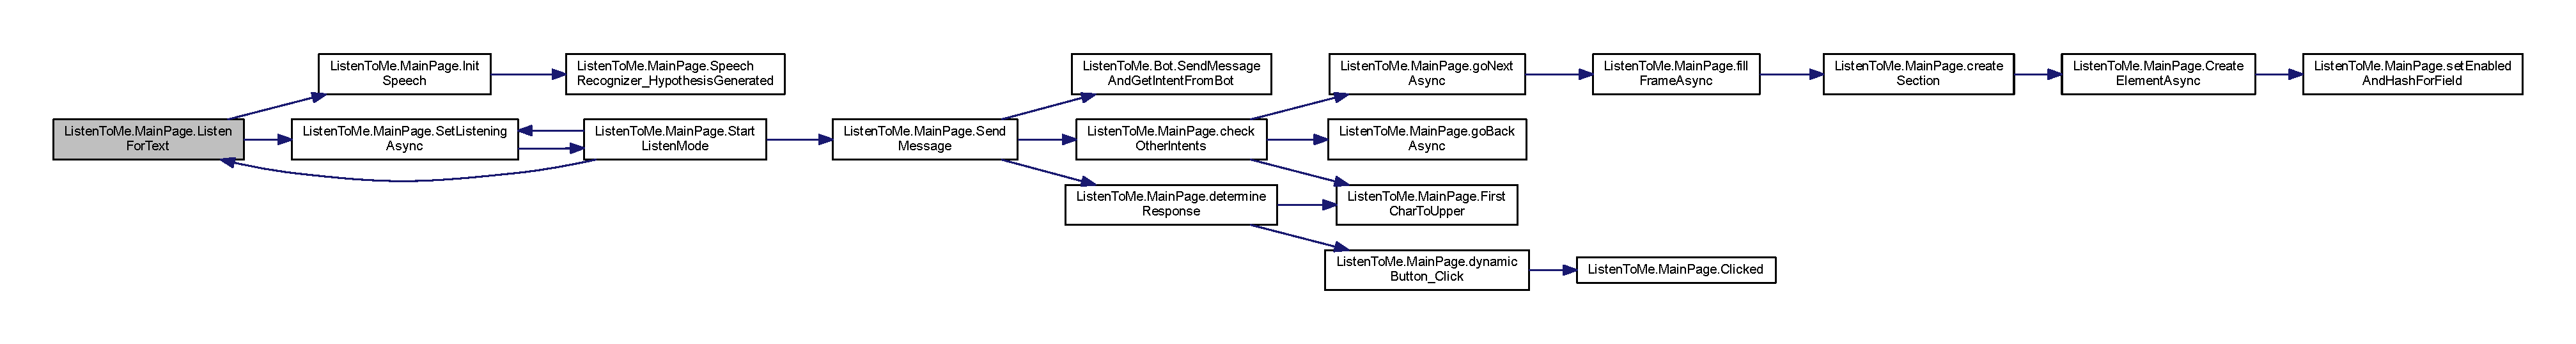
\includegraphics[width=350pt]{class_listen_to_me_1_1_main_page_a94a7dfd5dc1ec2e9bf7a86a4b9f7df0c_cgraph}
\end{center}
\end{figure}




Here is the caller graph for this function\+:
\nopagebreak
\begin{figure}[H]
\begin{center}
\leavevmode
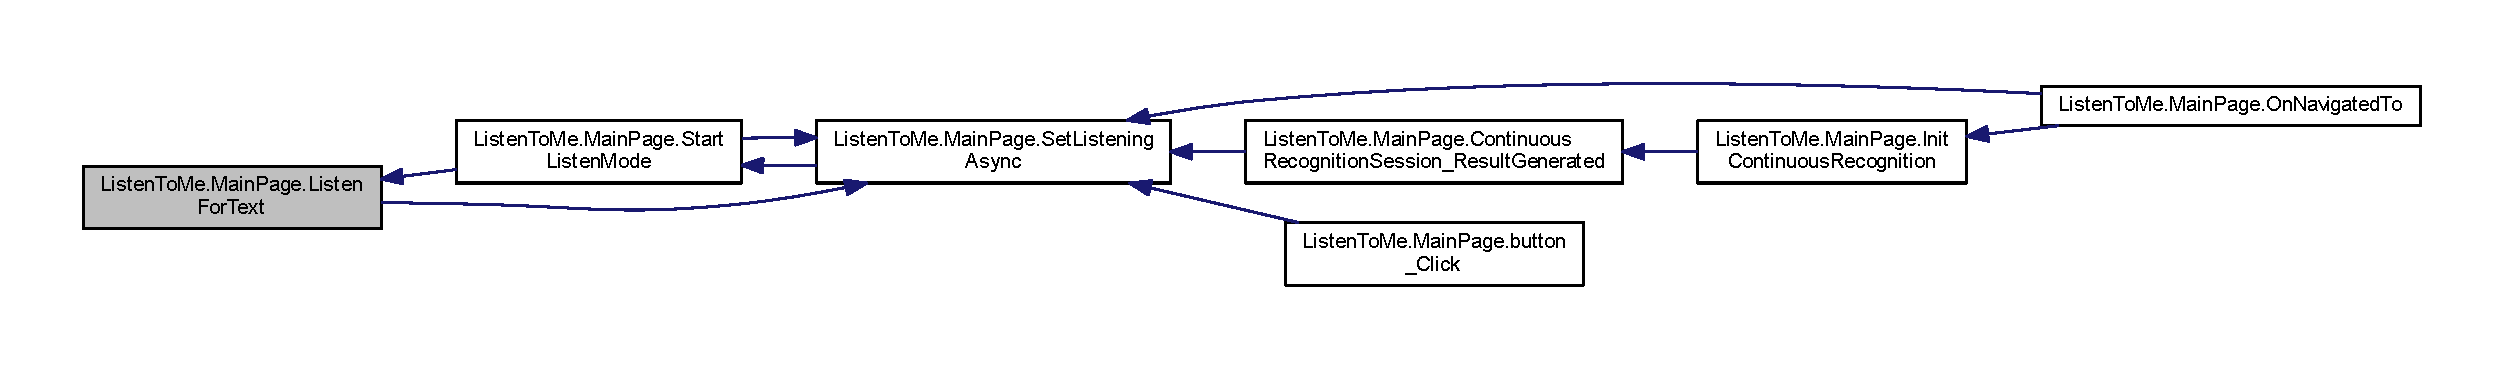
\includegraphics[width=350pt]{class_listen_to_me_1_1_main_page_a94a7dfd5dc1ec2e9bf7a86a4b9f7df0c_icgraph}
\end{center}
\end{figure}


\index{Listen\+To\+Me\+::\+Main\+Page@{Listen\+To\+Me\+::\+Main\+Page}!Media\+\_\+\+Media\+Ended@{Media\+\_\+\+Media\+Ended}}
\index{Media\+\_\+\+Media\+Ended@{Media\+\_\+\+Media\+Ended}!Listen\+To\+Me\+::\+Main\+Page@{Listen\+To\+Me\+::\+Main\+Page}}
\subsubsection[{\texorpdfstring{Media\+\_\+\+Media\+Ended(object sender, Routed\+Event\+Args e)}{Media_MediaEnded(object sender, RoutedEventArgs e)}}]{\setlength{\rightskip}{0pt plus 5cm}void Listen\+To\+Me.\+Main\+Page.\+Media\+\_\+\+Media\+Ended (
\begin{DoxyParamCaption}
\item[{object}]{sender, }
\item[{Routed\+Event\+Args}]{e}
\end{DoxyParamCaption}
)\hspace{0.3cm}{\ttfamily [private]}}\hypertarget{class_listen_to_me_1_1_main_page_ab7c9aeb7a6b1053375754c58933360d6}{}\label{class_listen_to_me_1_1_main_page_ab7c9aeb7a6b1053375754c58933360d6}


Here is the caller graph for this function\+:
\nopagebreak
\begin{figure}[H]
\begin{center}
\leavevmode
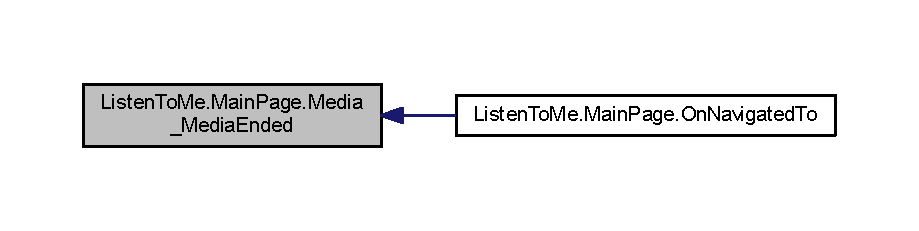
\includegraphics[width=350pt]{class_listen_to_me_1_1_main_page_ab7c9aeb7a6b1053375754c58933360d6_icgraph}
\end{center}
\end{figure}


\index{Listen\+To\+Me\+::\+Main\+Page@{Listen\+To\+Me\+::\+Main\+Page}!navigation\+Helper\+\_\+\+Load\+State@{navigation\+Helper\+\_\+\+Load\+State}}
\index{navigation\+Helper\+\_\+\+Load\+State@{navigation\+Helper\+\_\+\+Load\+State}!Listen\+To\+Me\+::\+Main\+Page@{Listen\+To\+Me\+::\+Main\+Page}}
\subsubsection[{\texorpdfstring{navigation\+Helper\+\_\+\+Load\+State(object sender, Load\+State\+Event\+Args e)}{navigationHelper_LoadState(object sender, LoadStateEventArgs e)}}]{\setlength{\rightskip}{0pt plus 5cm}void Listen\+To\+Me.\+Main\+Page.\+navigation\+Helper\+\_\+\+Load\+State (
\begin{DoxyParamCaption}
\item[{object}]{sender, }
\item[{Load\+State\+Event\+Args}]{e}
\end{DoxyParamCaption}
)\hspace{0.3cm}{\ttfamily [private]}}\hypertarget{class_listen_to_me_1_1_main_page_a696e8f4cb397c01ba2465d68e2b8c369}{}\label{class_listen_to_me_1_1_main_page_a696e8f4cb397c01ba2465d68e2b8c369}


to\+Do implement formstore call that loads the values of the input fields 


\begin{DoxyParams}{Parameters}
{\em sender} & \\
\hline
{\em e} & \\
\hline
\end{DoxyParams}


Here is the caller graph for this function\+:
\nopagebreak
\begin{figure}[H]
\begin{center}
\leavevmode
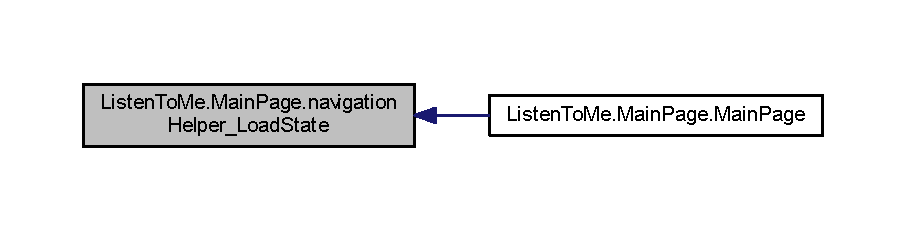
\includegraphics[width=350pt]{class_listen_to_me_1_1_main_page_a696e8f4cb397c01ba2465d68e2b8c369_icgraph}
\end{center}
\end{figure}


\index{Listen\+To\+Me\+::\+Main\+Page@{Listen\+To\+Me\+::\+Main\+Page}!navigation\+Helper\+\_\+\+Save\+State@{navigation\+Helper\+\_\+\+Save\+State}}
\index{navigation\+Helper\+\_\+\+Save\+State@{navigation\+Helper\+\_\+\+Save\+State}!Listen\+To\+Me\+::\+Main\+Page@{Listen\+To\+Me\+::\+Main\+Page}}
\subsubsection[{\texorpdfstring{navigation\+Helper\+\_\+\+Save\+State(object sender, Save\+State\+Event\+Args e)}{navigationHelper_SaveState(object sender, SaveStateEventArgs e)}}]{\setlength{\rightskip}{0pt plus 5cm}void Listen\+To\+Me.\+Main\+Page.\+navigation\+Helper\+\_\+\+Save\+State (
\begin{DoxyParamCaption}
\item[{object}]{sender, }
\item[{Save\+State\+Event\+Args}]{e}
\end{DoxyParamCaption}
)\hspace{0.3cm}{\ttfamily [private]}}\hypertarget{class_listen_to_me_1_1_main_page_abd810ebce6d7300369767bd604e107d2}{}\label{class_listen_to_me_1_1_main_page_abd810ebce6d7300369767bd604e107d2}


to\+Do implement formstore call that saves the values of the input fields 


\begin{DoxyParams}{Parameters}
{\em sender} & \\
\hline
{\em e} & \\
\hline
\end{DoxyParams}


Here is the caller graph for this function\+:
\nopagebreak
\begin{figure}[H]
\begin{center}
\leavevmode
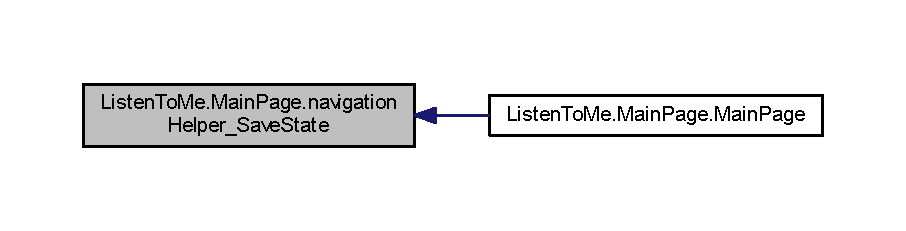
\includegraphics[width=350pt]{class_listen_to_me_1_1_main_page_abd810ebce6d7300369767bd604e107d2_icgraph}
\end{center}
\end{figure}


\index{Listen\+To\+Me\+::\+Main\+Page@{Listen\+To\+Me\+::\+Main\+Page}!Next\+Button\+\_\+\+Click@{Next\+Button\+\_\+\+Click}}
\index{Next\+Button\+\_\+\+Click@{Next\+Button\+\_\+\+Click}!Listen\+To\+Me\+::\+Main\+Page@{Listen\+To\+Me\+::\+Main\+Page}}
\subsubsection[{\texorpdfstring{Next\+Button\+\_\+\+Click(object sender, Routed\+Event\+Args e)}{NextButton_Click(object sender, RoutedEventArgs e)}}]{\setlength{\rightskip}{0pt plus 5cm}async void Listen\+To\+Me.\+Main\+Page.\+Next\+Button\+\_\+\+Click (
\begin{DoxyParamCaption}
\item[{object}]{sender, }
\item[{Routed\+Event\+Args}]{e}
\end{DoxyParamCaption}
)\hspace{0.3cm}{\ttfamily [private]}}\hypertarget{class_listen_to_me_1_1_main_page_a8144f2438fc2512708677190d74d2111}{}\label{class_listen_to_me_1_1_main_page_a8144f2438fc2512708677190d74d2111}


loads the next section into the frame 


\begin{DoxyParams}{Parameters}
{\em sender} & the next-\/button\\
\hline
{\em e} & some arguments\\
\hline
\end{DoxyParams}


Here is the call graph for this function\+:
\nopagebreak
\begin{figure}[H]
\begin{center}
\leavevmode
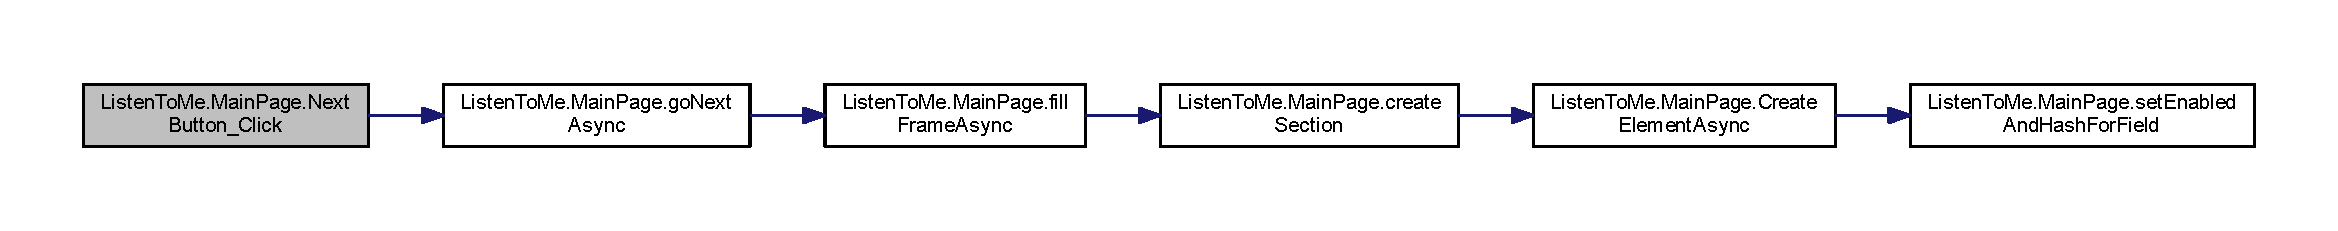
\includegraphics[width=350pt]{class_listen_to_me_1_1_main_page_a8144f2438fc2512708677190d74d2111_cgraph}
\end{center}
\end{figure}


\index{Listen\+To\+Me\+::\+Main\+Page@{Listen\+To\+Me\+::\+Main\+Page}!On\+Navigated\+From@{On\+Navigated\+From}}
\index{On\+Navigated\+From@{On\+Navigated\+From}!Listen\+To\+Me\+::\+Main\+Page@{Listen\+To\+Me\+::\+Main\+Page}}
\subsubsection[{\texorpdfstring{On\+Navigated\+From(\+Navigation\+Event\+Args e)}{OnNavigatedFrom(NavigationEventArgs e)}}]{\setlength{\rightskip}{0pt plus 5cm}override void Listen\+To\+Me.\+Main\+Page.\+On\+Navigated\+From (
\begin{DoxyParamCaption}
\item[{Navigation\+Event\+Args}]{e}
\end{DoxyParamCaption}
)\hspace{0.3cm}{\ttfamily [protected]}}\hypertarget{class_listen_to_me_1_1_main_page_a15a008ef01c6354ef72d4ec864d8d8e3}{}\label{class_listen_to_me_1_1_main_page_a15a008ef01c6354ef72d4ec864d8d8e3}
\index{Listen\+To\+Me\+::\+Main\+Page@{Listen\+To\+Me\+::\+Main\+Page}!On\+Navigated\+To@{On\+Navigated\+To}}
\index{On\+Navigated\+To@{On\+Navigated\+To}!Listen\+To\+Me\+::\+Main\+Page@{Listen\+To\+Me\+::\+Main\+Page}}
\subsubsection[{\texorpdfstring{On\+Navigated\+To(\+Navigation\+Event\+Args e)}{OnNavigatedTo(NavigationEventArgs e)}}]{\setlength{\rightskip}{0pt plus 5cm}override async void Listen\+To\+Me.\+Main\+Page.\+On\+Navigated\+To (
\begin{DoxyParamCaption}
\item[{Navigation\+Event\+Args}]{e}
\end{DoxyParamCaption}
)\hspace{0.3cm}{\ttfamily [protected]}}\hypertarget{class_listen_to_me_1_1_main_page_a8027d1a18b781cfe127ca02916c4552e}{}\label{class_listen_to_me_1_1_main_page_a8027d1a18b781cfe127ca02916c4552e}


is called after the login was sucessful 


\begin{DoxyParams}{Parameters}
{\em e} & \\
\hline
\end{DoxyParams}


Here is the call graph for this function\+:
\nopagebreak
\begin{figure}[H]
\begin{center}
\leavevmode
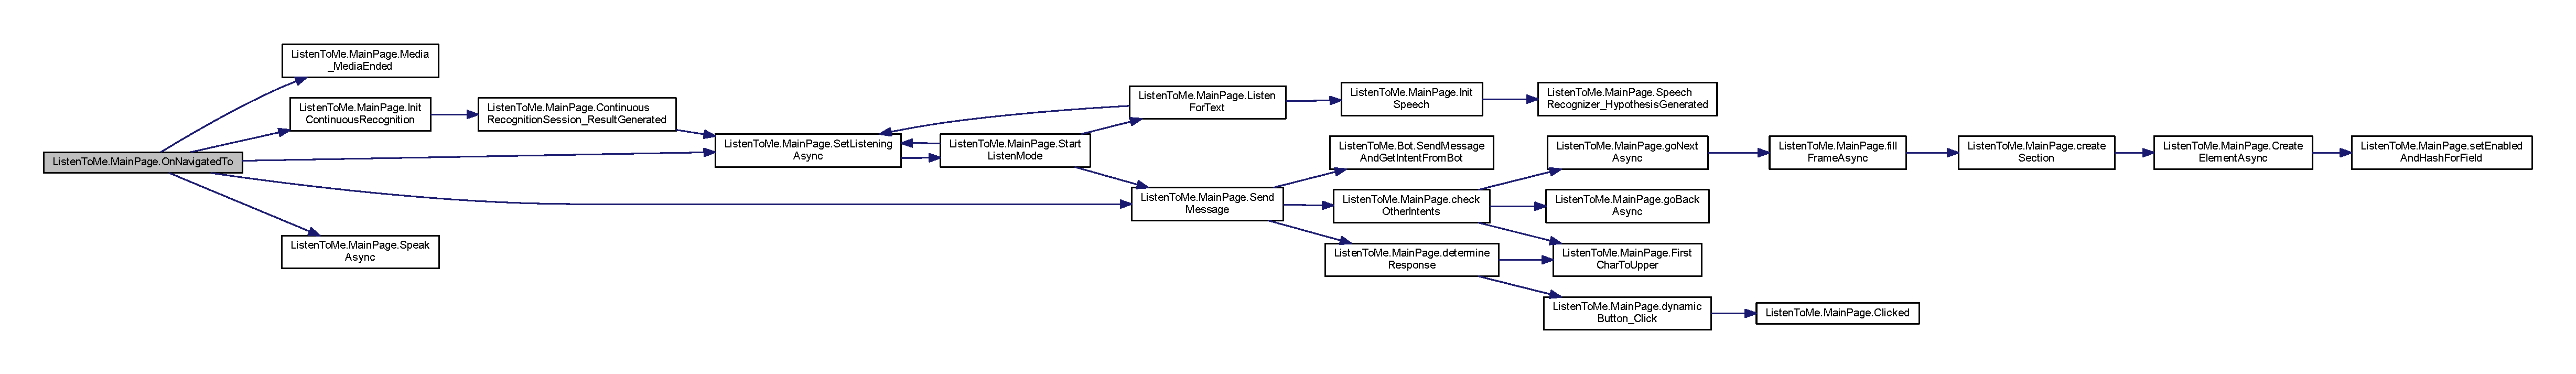
\includegraphics[width=350pt]{class_listen_to_me_1_1_main_page_a8027d1a18b781cfe127ca02916c4552e_cgraph}
\end{center}
\end{figure}


\index{Listen\+To\+Me\+::\+Main\+Page@{Listen\+To\+Me\+::\+Main\+Page}!Page\+\_\+\+Loaded@{Page\+\_\+\+Loaded}}
\index{Page\+\_\+\+Loaded@{Page\+\_\+\+Loaded}!Listen\+To\+Me\+::\+Main\+Page@{Listen\+To\+Me\+::\+Main\+Page}}
\subsubsection[{\texorpdfstring{Page\+\_\+\+Loaded(object sender, Routed\+Event\+Args e)}{Page_Loaded(object sender, RoutedEventArgs e)}}]{\setlength{\rightskip}{0pt plus 5cm}void Listen\+To\+Me.\+Main\+Page.\+Page\+\_\+\+Loaded (
\begin{DoxyParamCaption}
\item[{object}]{sender, }
\item[{Routed\+Event\+Args}]{e}
\end{DoxyParamCaption}
)\hspace{0.3cm}{\ttfamily [private]}}\hypertarget{class_listen_to_me_1_1_main_page_a9e7a645ae278f0e83ff9c3a831b37028}{}\label{class_listen_to_me_1_1_main_page_a9e7a645ae278f0e83ff9c3a831b37028}
\index{Listen\+To\+Me\+::\+Main\+Page@{Listen\+To\+Me\+::\+Main\+Page}!Send\+Message@{Send\+Message}}
\index{Send\+Message@{Send\+Message}!Listen\+To\+Me\+::\+Main\+Page@{Listen\+To\+Me\+::\+Main\+Page}}
\subsubsection[{\texorpdfstring{Send\+Message(string message, bool speak=false)}{SendMessage(string message, bool speak=false)}}]{\setlength{\rightskip}{0pt plus 5cm}async void Listen\+To\+Me.\+Main\+Page.\+Send\+Message (
\begin{DoxyParamCaption}
\item[{string}]{message, }
\item[{bool}]{speak = {\ttfamily false}}
\end{DoxyParamCaption}
)\hspace{0.3cm}{\ttfamily [private]}}\hypertarget{class_listen_to_me_1_1_main_page_a09c2518852d4261ff6a2118c8e01de9f}{}\label{class_listen_to_me_1_1_main_page_a09c2518852d4261ff6a2118c8e01de9f}


calls the L\+U\+IS A\+PI to retrieve the \hyperlink{class_listen_to_me_1_1_bot}{Bot} Web\+App\textquotesingle{}s answer for a specific request 


\begin{DoxyParams}{Parameters}
{\em message} & the request\\
\hline
{\em speak} & flag that indicates whether the funtion is called in speech mode or text mode\\
\hline
\end{DoxyParams}


Here is the call graph for this function\+:
\nopagebreak
\begin{figure}[H]
\begin{center}
\leavevmode
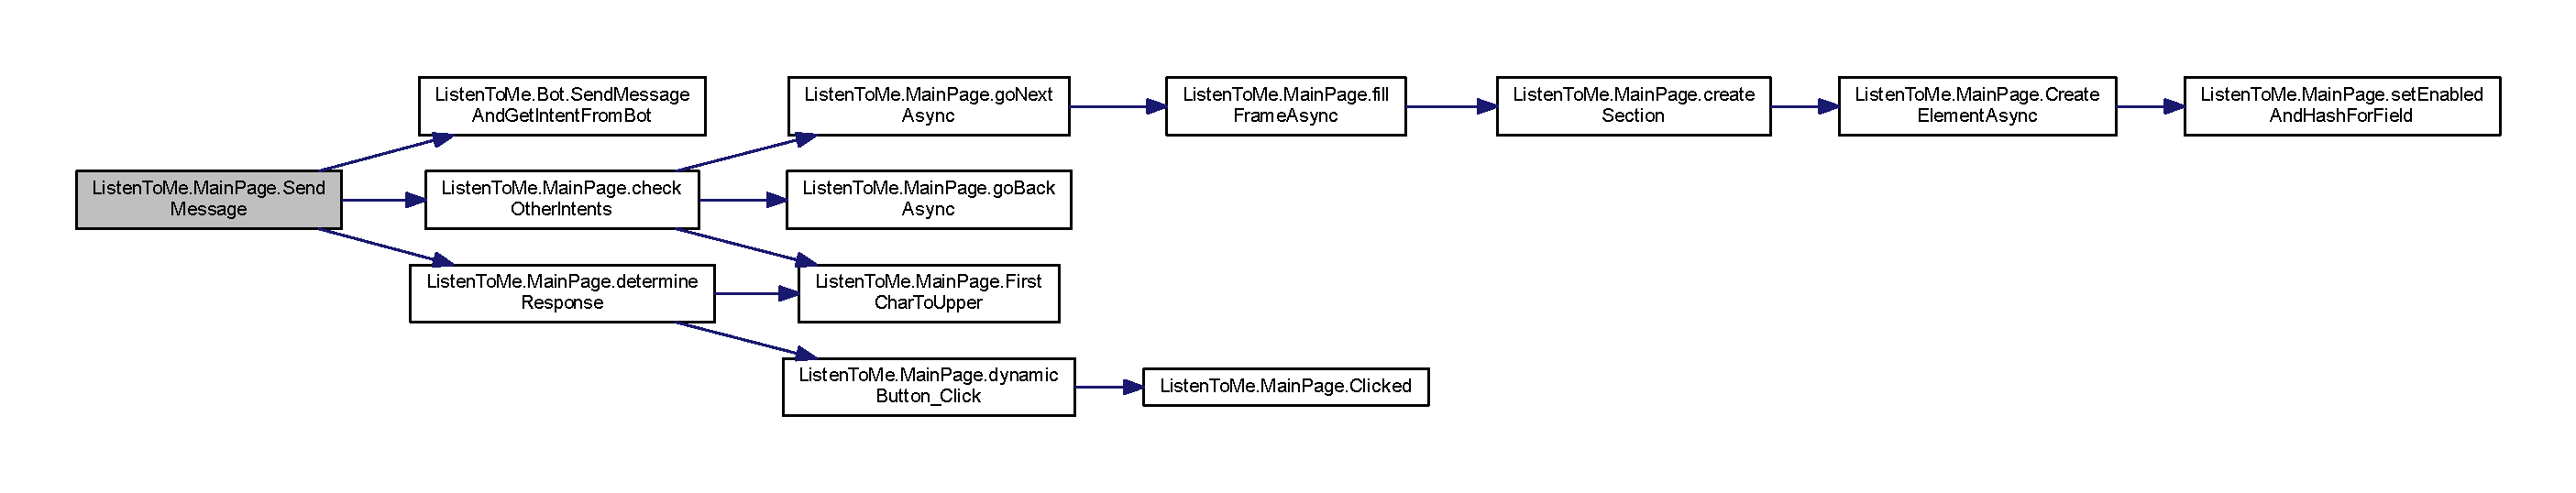
\includegraphics[width=350pt]{class_listen_to_me_1_1_main_page_a09c2518852d4261ff6a2118c8e01de9f_cgraph}
\end{center}
\end{figure}




Here is the caller graph for this function\+:
\nopagebreak
\begin{figure}[H]
\begin{center}
\leavevmode
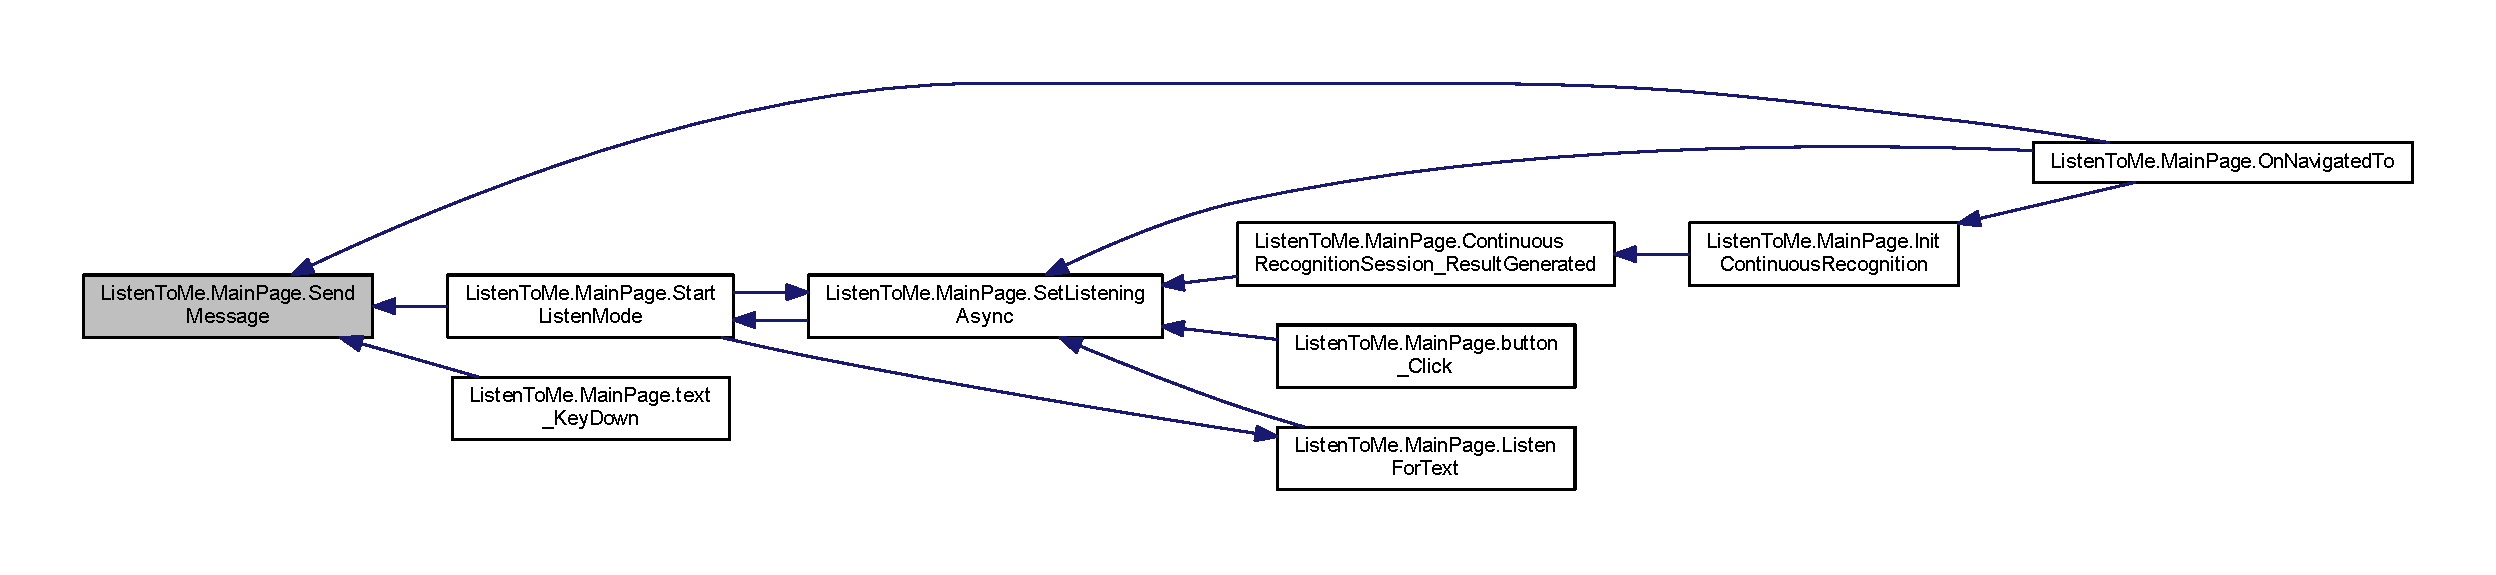
\includegraphics[width=350pt]{class_listen_to_me_1_1_main_page_a09c2518852d4261ff6a2118c8e01de9f_icgraph}
\end{center}
\end{figure}


\index{Listen\+To\+Me\+::\+Main\+Page@{Listen\+To\+Me\+::\+Main\+Page}!set\+Enabled\+And\+Hash\+For\+Field@{set\+Enabled\+And\+Hash\+For\+Field}}
\index{set\+Enabled\+And\+Hash\+For\+Field@{set\+Enabled\+And\+Hash\+For\+Field}!Listen\+To\+Me\+::\+Main\+Page@{Listen\+To\+Me\+::\+Main\+Page}}
\subsubsection[{\texorpdfstring{set\+Enabled\+And\+Hash\+For\+Field(\+Text\+Box field, Element element, Stack\+Panel panel)}{setEnabledAndHashForField(TextBox field, Element element, StackPanel panel)}}]{\setlength{\rightskip}{0pt plus 5cm}void Listen\+To\+Me.\+Main\+Page.\+set\+Enabled\+And\+Hash\+For\+Field (
\begin{DoxyParamCaption}
\item[{Text\+Box}]{field, }
\item[{Element}]{element, }
\item[{Stack\+Panel}]{panel}
\end{DoxyParamCaption}
)\hspace{0.3cm}{\ttfamily [private]}}\hypertarget{class_listen_to_me_1_1_main_page_a80911257473f608abc125a1083045041}{}\label{class_listen_to_me_1_1_main_page_a80911257473f608abc125a1083045041}


sets the enabled property of a Text\+Box control to disabled, if the model Element\textquotesingle{}s property is set to \textquotesingle{}disabled\textquotesingle{} string. This is the case for input elements that are only for displaying information, e.\+g. summing up other entries made by the user. If the Text\+Box stays enabled, the header will be added to the Hash\+Table that is used by the L\+U\+I\+S-\/\+Model to determine to which Text\+Box to pass a user value to. 


\begin{DoxyParams}{Parameters}
{\em field} & The Text\+Box to be set\\
\hline
{\em element} & the model insatnce that saved the future property valus of the field\\
\hline
{\em panel} & the panel on which all Text\+Boxes lie\\
\hline
\end{DoxyParams}


Here is the caller graph for this function\+:
\nopagebreak
\begin{figure}[H]
\begin{center}
\leavevmode
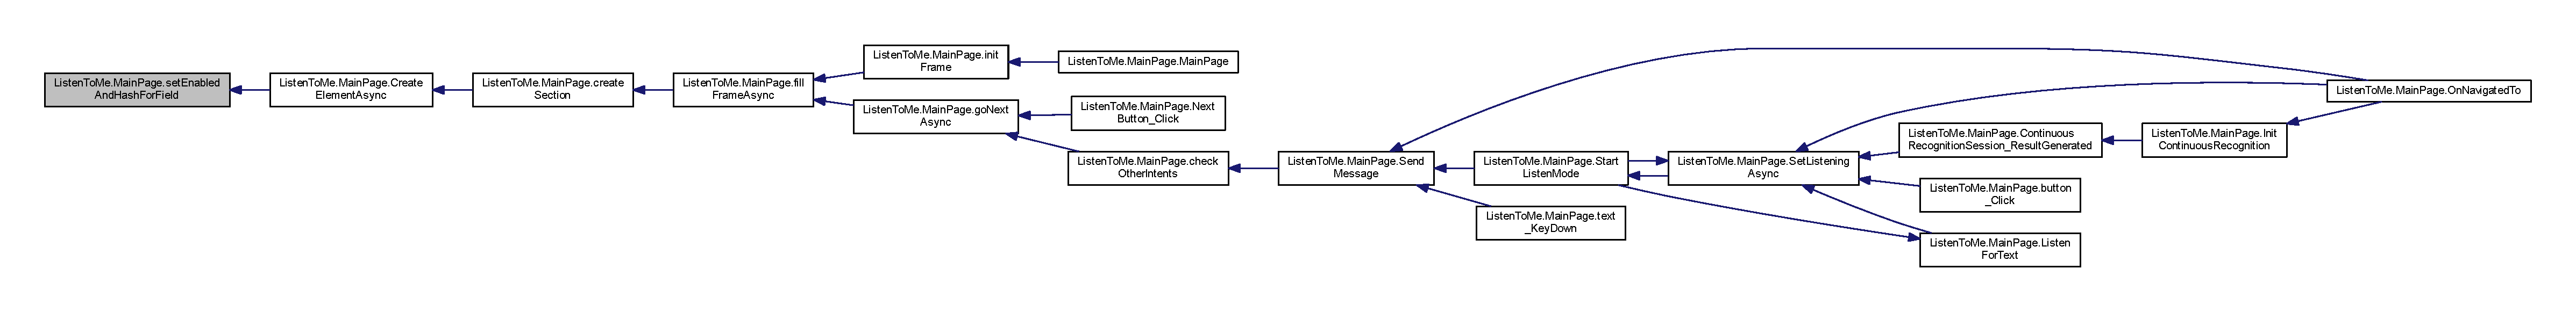
\includegraphics[width=350pt]{class_listen_to_me_1_1_main_page_a80911257473f608abc125a1083045041_icgraph}
\end{center}
\end{figure}


\index{Listen\+To\+Me\+::\+Main\+Page@{Listen\+To\+Me\+::\+Main\+Page}!Set\+Listening\+Async@{Set\+Listening\+Async}}
\index{Set\+Listening\+Async@{Set\+Listening\+Async}!Listen\+To\+Me\+::\+Main\+Page@{Listen\+To\+Me\+::\+Main\+Page}}
\subsubsection[{\texorpdfstring{Set\+Listening\+Async(bool to\+Listen)}{SetListeningAsync(bool toListen)}}]{\setlength{\rightskip}{0pt plus 5cm}async System.\+Threading.\+Tasks.\+Task Listen\+To\+Me.\+Main\+Page.\+Set\+Listening\+Async (
\begin{DoxyParamCaption}
\item[{bool}]{to\+Listen}
\end{DoxyParamCaption}
)\hspace{0.3cm}{\ttfamily [private]}}\hypertarget{class_listen_to_me_1_1_main_page_a57d75ef6bb9c10b0c944c3eb5513b076}{}\label{class_listen_to_me_1_1_main_page_a57d75ef6bb9c10b0c944c3eb5513b076}


sets the flag whether speech recognition is enabled according to the parameter 


\begin{DoxyParams}{Parameters}
{\em to\+Listen} & the parameter. If true it sets the flag and activates listenmode for false vice versa\\
\hline
\end{DoxyParams}
\begin{DoxyReturn}{Returns}

\end{DoxyReturn}


Here is the call graph for this function\+:
\nopagebreak
\begin{figure}[H]
\begin{center}
\leavevmode
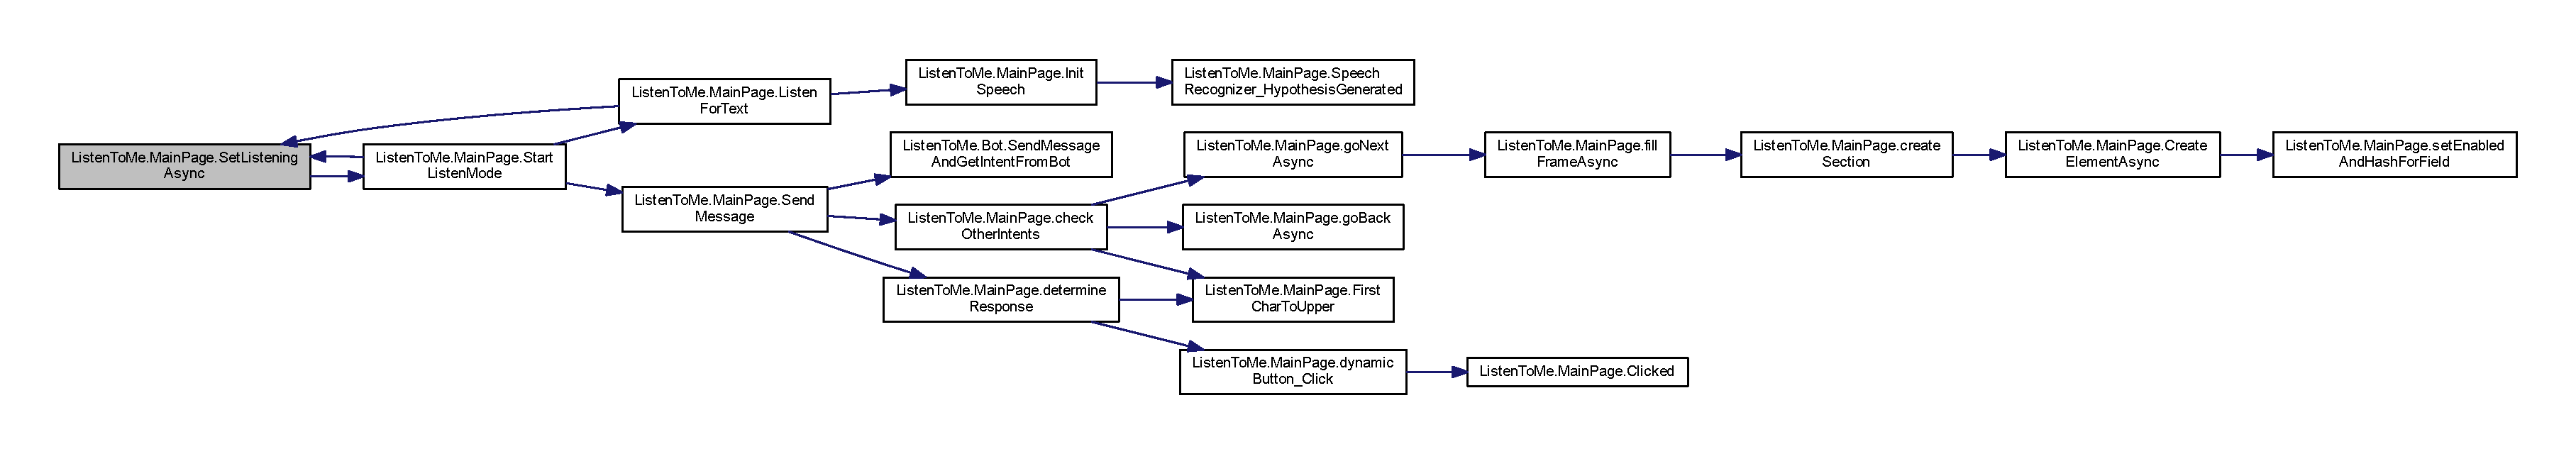
\includegraphics[width=350pt]{class_listen_to_me_1_1_main_page_a57d75ef6bb9c10b0c944c3eb5513b076_cgraph}
\end{center}
\end{figure}




Here is the caller graph for this function\+:
\nopagebreak
\begin{figure}[H]
\begin{center}
\leavevmode
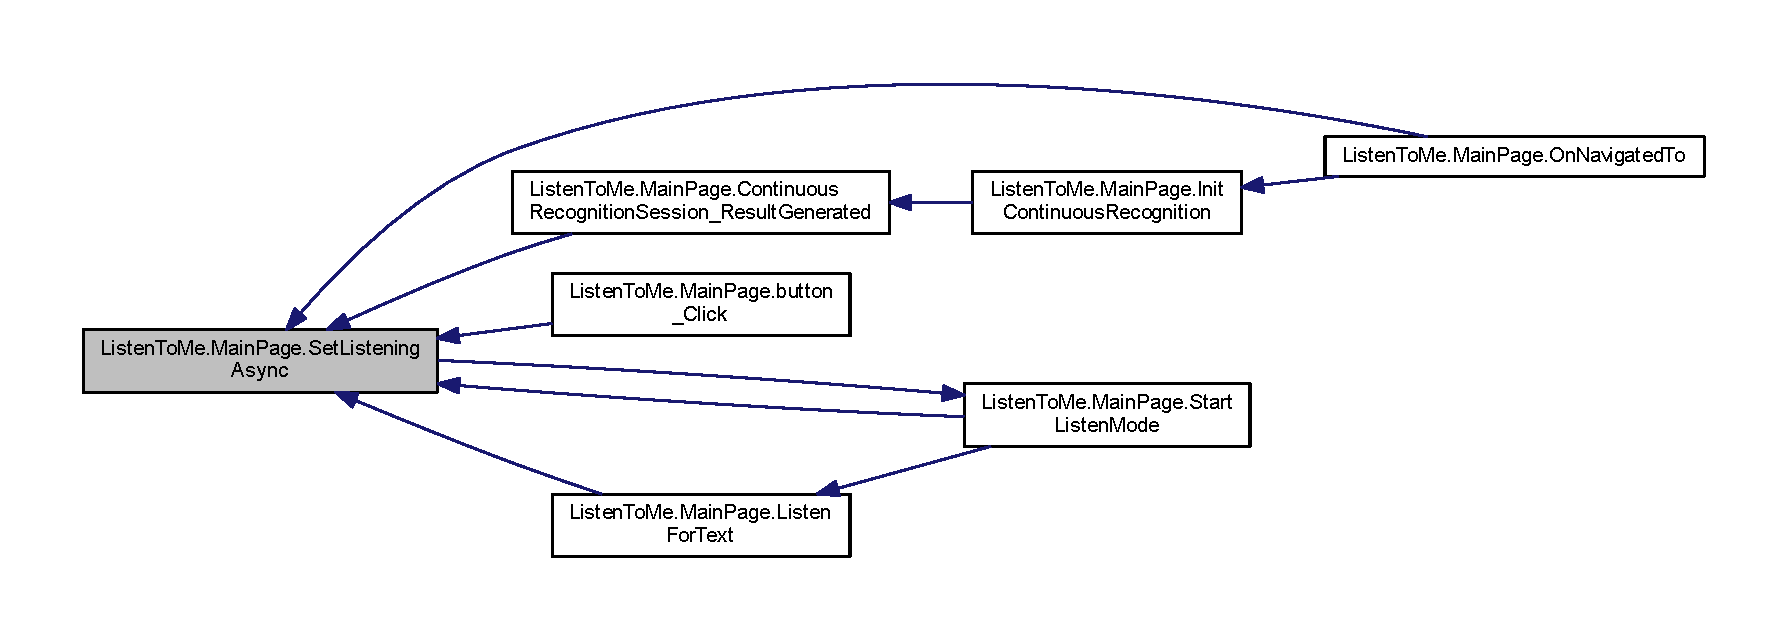
\includegraphics[width=350pt]{class_listen_to_me_1_1_main_page_a57d75ef6bb9c10b0c944c3eb5513b076_icgraph}
\end{center}
\end{figure}


\index{Listen\+To\+Me\+::\+Main\+Page@{Listen\+To\+Me\+::\+Main\+Page}!Speak\+Async@{Speak\+Async}}
\index{Speak\+Async@{Speak\+Async}!Listen\+To\+Me\+::\+Main\+Page@{Listen\+To\+Me\+::\+Main\+Page}}
\subsubsection[{\texorpdfstring{Speak\+Async(string to\+Speak)}{SpeakAsync(string toSpeak)}}]{\setlength{\rightskip}{0pt plus 5cm}async Task Listen\+To\+Me.\+Main\+Page.\+Speak\+Async (
\begin{DoxyParamCaption}
\item[{string}]{to\+Speak}
\end{DoxyParamCaption}
)\hspace{0.3cm}{\ttfamily [private]}}\hypertarget{class_listen_to_me_1_1_main_page_aa1c50f04230b8907027a95bfe54cb7d2}{}\label{class_listen_to_me_1_1_main_page_aa1c50f04230b8907027a95bfe54cb7d2}


lets the \hyperlink{class_listen_to_me_1_1_app}{App} speak the answer to the user 


\begin{DoxyParams}{Parameters}
{\em to\+Speak} & the answer to be spoken\\
\hline
\end{DoxyParams}


Here is the caller graph for this function\+:
\nopagebreak
\begin{figure}[H]
\begin{center}
\leavevmode
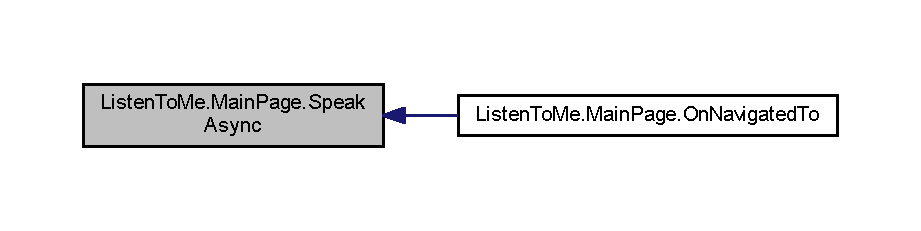
\includegraphics[width=350pt]{class_listen_to_me_1_1_main_page_aa1c50f04230b8907027a95bfe54cb7d2_icgraph}
\end{center}
\end{figure}


\index{Listen\+To\+Me\+::\+Main\+Page@{Listen\+To\+Me\+::\+Main\+Page}!Speech\+Recognizer\+\_\+\+Hypothesis\+Generated@{Speech\+Recognizer\+\_\+\+Hypothesis\+Generated}}
\index{Speech\+Recognizer\+\_\+\+Hypothesis\+Generated@{Speech\+Recognizer\+\_\+\+Hypothesis\+Generated}!Listen\+To\+Me\+::\+Main\+Page@{Listen\+To\+Me\+::\+Main\+Page}}
\subsubsection[{\texorpdfstring{Speech\+Recognizer\+\_\+\+Hypothesis\+Generated(\+Speech\+Recognizer sender, Speech\+Recognition\+Hypothesis\+Generated\+Event\+Args args)}{SpeechRecognizer_HypothesisGenerated(SpeechRecognizer sender, SpeechRecognitionHypothesisGeneratedEventArgs args)}}]{\setlength{\rightskip}{0pt plus 5cm}async void Listen\+To\+Me.\+Main\+Page.\+Speech\+Recognizer\+\_\+\+Hypothesis\+Generated (
\begin{DoxyParamCaption}
\item[{Speech\+Recognizer}]{sender, }
\item[{Speech\+Recognition\+Hypothesis\+Generated\+Event\+Args}]{args}
\end{DoxyParamCaption}
)\hspace{0.3cm}{\ttfamily [private]}}\hypertarget{class_listen_to_me_1_1_main_page_a78024cb9b68bafc3375081574dbbea89}{}\label{class_listen_to_me_1_1_main_page_a78024cb9b68bafc3375081574dbbea89}


handles the Hypothesis\+Generated event of the speech recognizer 


\begin{DoxyParams}{Parameters}
{\em sender} & the speech recognizer\\
\hline
{\em args} & arguments that may be passed\\
\hline
\end{DoxyParams}


Here is the caller graph for this function\+:
\nopagebreak
\begin{figure}[H]
\begin{center}
\leavevmode
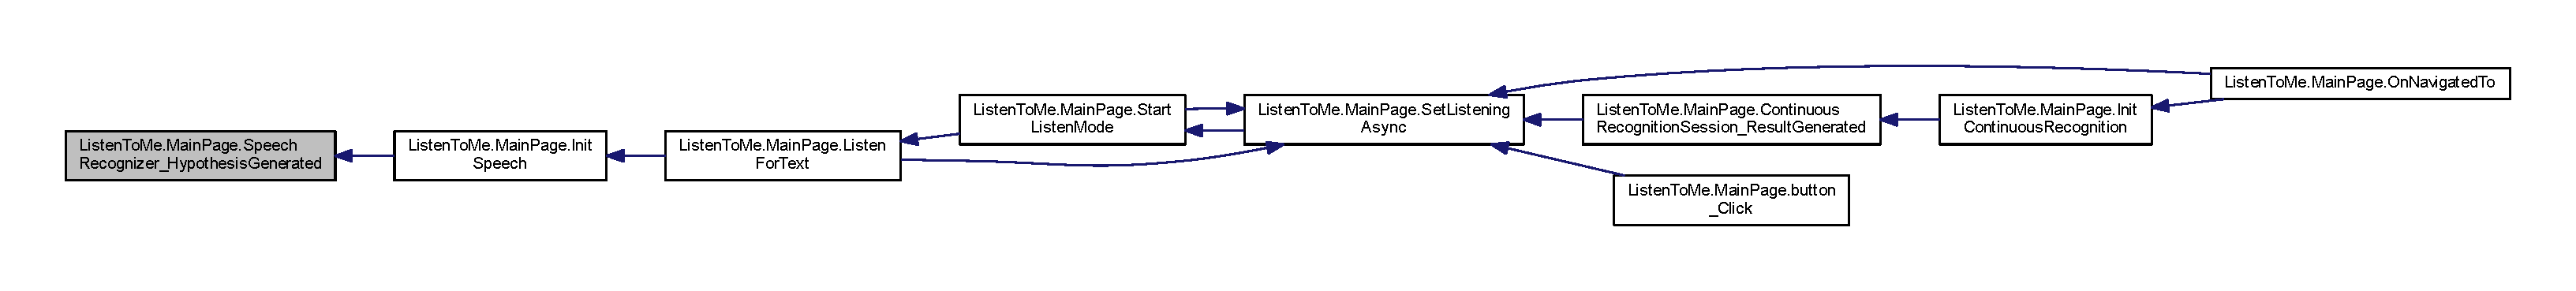
\includegraphics[width=350pt]{class_listen_to_me_1_1_main_page_a78024cb9b68bafc3375081574dbbea89_icgraph}
\end{center}
\end{figure}


\index{Listen\+To\+Me\+::\+Main\+Page@{Listen\+To\+Me\+::\+Main\+Page}!Start\+Listen\+Mode@{Start\+Listen\+Mode}}
\index{Start\+Listen\+Mode@{Start\+Listen\+Mode}!Listen\+To\+Me\+::\+Main\+Page@{Listen\+To\+Me\+::\+Main\+Page}}
\subsubsection[{\texorpdfstring{Start\+Listen\+Mode()}{StartListenMode()}}]{\setlength{\rightskip}{0pt plus 5cm}async void Listen\+To\+Me.\+Main\+Page.\+Start\+Listen\+Mode (
\begin{DoxyParamCaption}
{}
\end{DoxyParamCaption}
)\hspace{0.3cm}{\ttfamily [private]}}\hypertarget{class_listen_to_me_1_1_main_page_ab9fba04f0fc94773c2838f6af87ec14b}{}\label{class_listen_to_me_1_1_main_page_ab9fba04f0fc94773c2838f6af87ec14b}


analyzes the speech input, recognized the text and calls \hyperlink{class_listen_to_me_1_1_main_page_a09c2518852d4261ff6a2118c8e01de9f}{Send\+Message()} to display the rcognized text 



Here is the call graph for this function\+:
\nopagebreak
\begin{figure}[H]
\begin{center}
\leavevmode
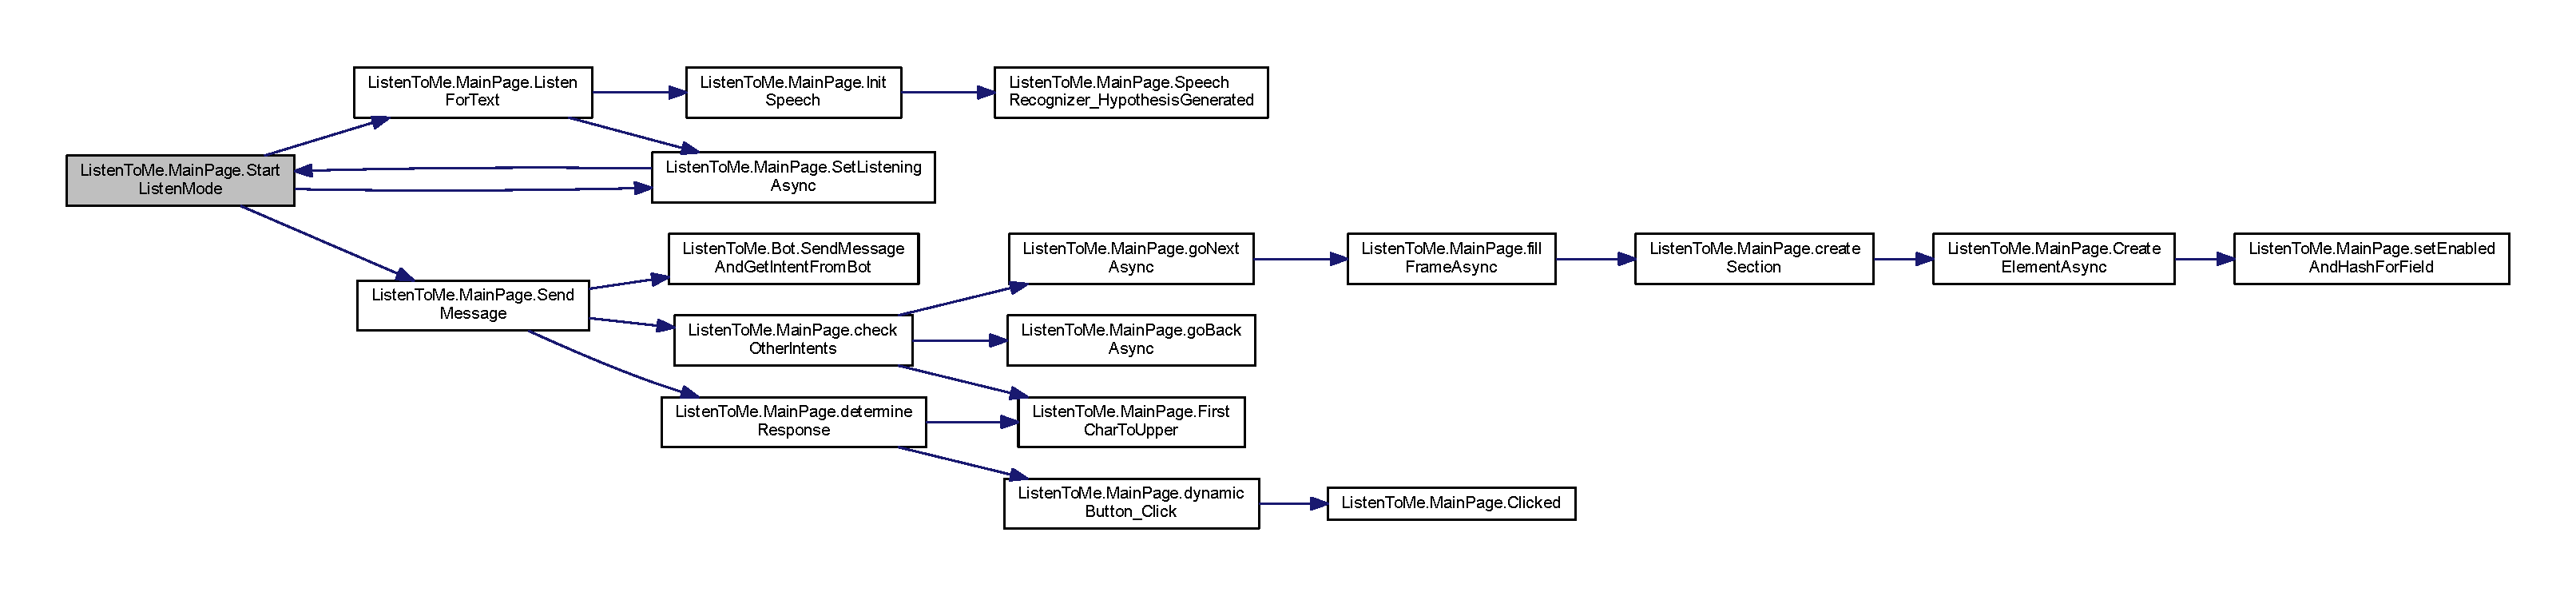
\includegraphics[width=350pt]{class_listen_to_me_1_1_main_page_ab9fba04f0fc94773c2838f6af87ec14b_cgraph}
\end{center}
\end{figure}




Here is the caller graph for this function\+:
\nopagebreak
\begin{figure}[H]
\begin{center}
\leavevmode
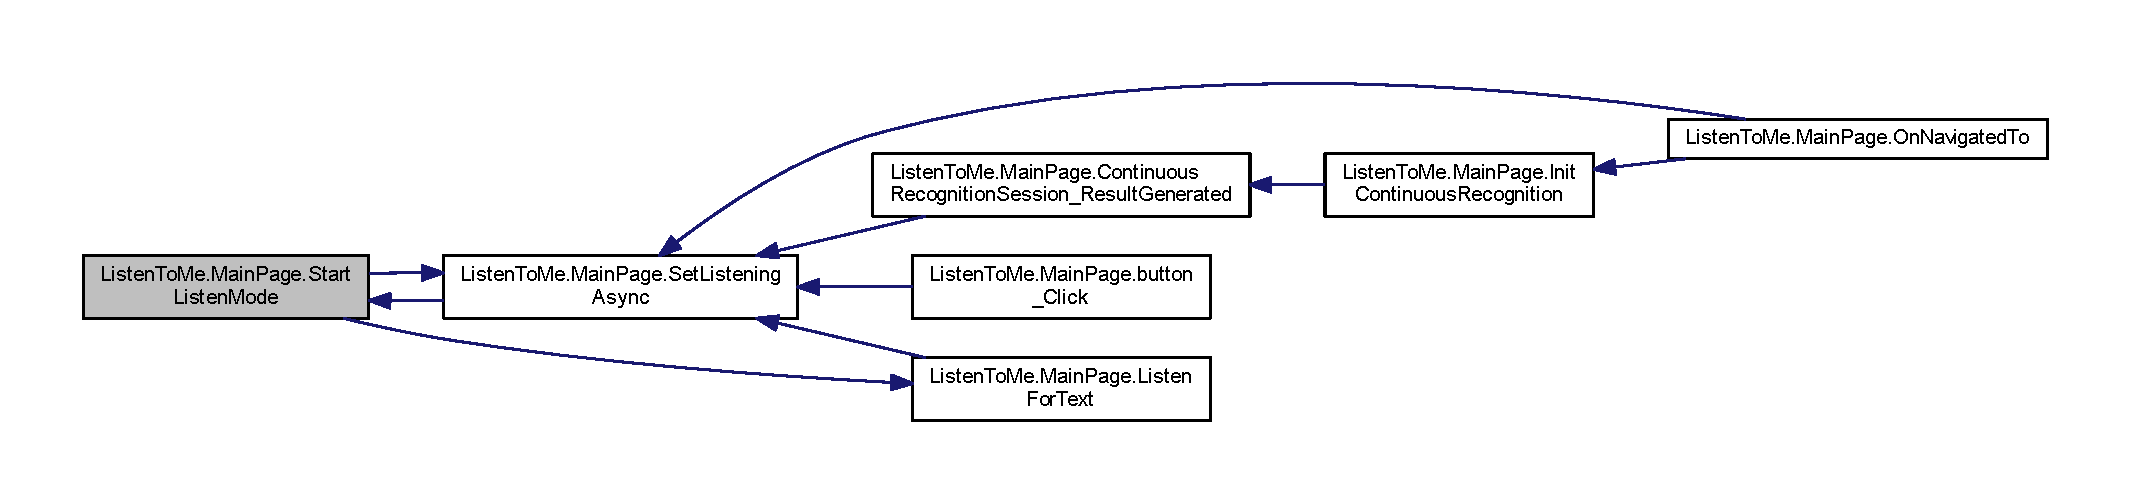
\includegraphics[width=350pt]{class_listen_to_me_1_1_main_page_ab9fba04f0fc94773c2838f6af87ec14b_icgraph}
\end{center}
\end{figure}


\index{Listen\+To\+Me\+::\+Main\+Page@{Listen\+To\+Me\+::\+Main\+Page}!test\+Net\+Connection\+Smaller@{test\+Net\+Connection\+Smaller}}
\index{test\+Net\+Connection\+Smaller@{test\+Net\+Connection\+Smaller}!Listen\+To\+Me\+::\+Main\+Page@{Listen\+To\+Me\+::\+Main\+Page}}
\subsubsection[{\texorpdfstring{test\+Net\+Connection\+Smaller()}{testNetConnectionSmaller()}}]{\setlength{\rightskip}{0pt plus 5cm}async void Listen\+To\+Me.\+Main\+Page.\+test\+Net\+Connection\+Smaller (
\begin{DoxyParamCaption}
{}
\end{DoxyParamCaption}
)}\hypertarget{class_listen_to_me_1_1_main_page_a4adb881a143354b71604cfa79ea69e25}{}\label{class_listen_to_me_1_1_main_page_a4adb881a143354b71604cfa79ea69e25}


testing connection to the website. Not working, both requests return with empty responses. reference\+: \href{https://blogs.windows.com/buildingapps/2015/11/23/demystifying-httpclient-apis-in-the-universal-windows-platform/#kzmsLAKtjKLGJFAU.97}{\tt https\+://blogs.\+windows.\+com/buildingapps/2015/11/23/demystifying-\/httpclient-\/apis-\/in-\/the-\/universal-\/windows-\/platform/\#kzms\+L\+A\+Ktj\+K\+L\+G\+J\+F\+A\+U.\+97} reference\+: \href{https://docs.microsoft.com/en-us/aspnet/web-api/overview/advanced/calling-a-web-api-from-a-net-client}{\tt https\+://docs.\+microsoft.\+com/en-\/us/aspnet/web-\/api/overview/advanced/calling-\/a-\/web-\/api-\/from-\/a-\/net-\/client} 


\begin{DoxyParams}{Parameters}
{\em user\+Name} & \\
\hline
{\em password} & \\
\hline
\end{DoxyParams}
\index{Listen\+To\+Me\+::\+Main\+Page@{Listen\+To\+Me\+::\+Main\+Page}!test\+Regex@{test\+Regex}}
\index{test\+Regex@{test\+Regex}!Listen\+To\+Me\+::\+Main\+Page@{Listen\+To\+Me\+::\+Main\+Page}}
\subsubsection[{\texorpdfstring{test\+Regex()}{testRegex()}}]{\setlength{\rightskip}{0pt plus 5cm}async void Listen\+To\+Me.\+Main\+Page.\+test\+Regex (
\begin{DoxyParamCaption}
{}
\end{DoxyParamCaption}
)\hspace{0.3cm}{\ttfamily [private]}}\hypertarget{class_listen_to_me_1_1_main_page_ae285c1eb3d44999ceecdb1b4f5a7bf83}{}\label{class_listen_to_me_1_1_main_page_ae285c1eb3d44999ceecdb1b4f5a7bf83}
\index{Listen\+To\+Me\+::\+Main\+Page@{Listen\+To\+Me\+::\+Main\+Page}!text\+\_\+\+Key\+Down@{text\+\_\+\+Key\+Down}}
\index{text\+\_\+\+Key\+Down@{text\+\_\+\+Key\+Down}!Listen\+To\+Me\+::\+Main\+Page@{Listen\+To\+Me\+::\+Main\+Page}}
\subsubsection[{\texorpdfstring{text\+\_\+\+Key\+Down(object sender, Key\+Routed\+Event\+Args e)}{text_KeyDown(object sender, KeyRoutedEventArgs e)}}]{\setlength{\rightskip}{0pt plus 5cm}void Listen\+To\+Me.\+Main\+Page.\+text\+\_\+\+Key\+Down (
\begin{DoxyParamCaption}
\item[{object}]{sender, }
\item[{Key\+Routed\+Event\+Args}]{e}
\end{DoxyParamCaption}
)\hspace{0.3cm}{\ttfamily [private]}}\hypertarget{class_listen_to_me_1_1_main_page_a2b101dc0c72c1dcb73fe756a5847940e}{}\label{class_listen_to_me_1_1_main_page_a2b101dc0c72c1dcb73fe756a5847940e}


Method that is reacting each time a key is hit while the textinput field has focus. 


\begin{DoxyParams}{Parameters}
{\em sender} & \\
\hline
{\em e} & \\
\hline
\end{DoxyParams}


Here is the call graph for this function\+:
\nopagebreak
\begin{figure}[H]
\begin{center}
\leavevmode
\includegraphics[width=350pt]{class_listen_to_me_1_1_main_page_a2b101dc0c72c1dcb73fe756a5847940e_cgraph}
\end{center}
\end{figure}




\subsection{Member Data Documentation}
\index{Listen\+To\+Me\+::\+Main\+Page@{Listen\+To\+Me\+::\+Main\+Page}!bot@{bot}}
\index{bot@{bot}!Listen\+To\+Me\+::\+Main\+Page@{Listen\+To\+Me\+::\+Main\+Page}}
\subsubsection[{\texorpdfstring{bot}{bot}}]{\setlength{\rightskip}{0pt plus 5cm}{\bf Bot} Listen\+To\+Me.\+Main\+Page.\+bot\hspace{0.3cm}{\ttfamily [private]}}\hypertarget{class_listen_to_me_1_1_main_page_a09b9deff7e80e3d524cd0f12d1c060f9}{}\label{class_listen_to_me_1_1_main_page_a09b9deff7e80e3d524cd0f12d1c060f9}


connects via Direct\+Line tho the Web\+App. Communicates with the language understanding intelligence model 

\index{Listen\+To\+Me\+::\+Main\+Page@{Listen\+To\+Me\+::\+Main\+Page}!count\+User\+Inputs@{count\+User\+Inputs}}
\index{count\+User\+Inputs@{count\+User\+Inputs}!Listen\+To\+Me\+::\+Main\+Page@{Listen\+To\+Me\+::\+Main\+Page}}
\subsubsection[{\texorpdfstring{count\+User\+Inputs}{countUserInputs}}]{\setlength{\rightskip}{0pt plus 5cm}int Listen\+To\+Me.\+Main\+Page.\+count\+User\+Inputs\hspace{0.3cm}{\ttfamily [private]}}\hypertarget{class_listen_to_me_1_1_main_page_a94ae31ea5ea90fff0194c7c3345e3987}{}\label{class_listen_to_me_1_1_main_page_a94ae31ea5ea90fff0194c7c3345e3987}


counts the user\textquotesingle{}s inputs for helping the app at guessing which field is filled out next. 

\index{Listen\+To\+Me\+::\+Main\+Page@{Listen\+To\+Me\+::\+Main\+Page}!current\+Panel@{current\+Panel}}
\index{current\+Panel@{current\+Panel}!Listen\+To\+Me\+::\+Main\+Page@{Listen\+To\+Me\+::\+Main\+Page}}
\subsubsection[{\texorpdfstring{current\+Panel}{currentPanel}}]{\setlength{\rightskip}{0pt plus 5cm}Stack\+Panel Listen\+To\+Me.\+Main\+Page.\+current\+Panel\hspace{0.3cm}{\ttfamily [private]}}\hypertarget{class_listen_to_me_1_1_main_page_a6dbd09c74d99bf0223489a06035980eb}{}\label{class_listen_to_me_1_1_main_page_a6dbd09c74d99bf0223489a06035980eb}


contains the Text\+Boxes and other controls of the page 

\index{Listen\+To\+Me\+::\+Main\+Page@{Listen\+To\+Me\+::\+Main\+Page}!index\+Of\+Current\+Element@{index\+Of\+Current\+Element}}
\index{index\+Of\+Current\+Element@{index\+Of\+Current\+Element}!Listen\+To\+Me\+::\+Main\+Page@{Listen\+To\+Me\+::\+Main\+Page}}
\subsubsection[{\texorpdfstring{index\+Of\+Current\+Element}{indexOfCurrentElement}}]{\setlength{\rightskip}{0pt plus 5cm}int Listen\+To\+Me.\+Main\+Page.\+index\+Of\+Current\+Element\hspace{0.3cm}{\ttfamily [private]}}\hypertarget{class_listen_to_me_1_1_main_page_acc0f3cb24ff26c2cfc76cd42a2fe2118}{}\label{class_listen_to_me_1_1_main_page_acc0f3cb24ff26c2cfc76cd42a2fe2118}


index of the last Text\+Box to which text was send with \hyperlink{class_listen_to_me_1_1_main_page_a09c2518852d4261ff6a2118c8e01de9f}{Send\+Message(string, bool)} 

\index{Listen\+To\+Me\+::\+Main\+Page@{Listen\+To\+Me\+::\+Main\+Page}!inputs@{inputs}}
\index{inputs@{inputs}!Listen\+To\+Me\+::\+Main\+Page@{Listen\+To\+Me\+::\+Main\+Page}}
\subsubsection[{\texorpdfstring{inputs}{inputs}}]{\setlength{\rightskip}{0pt plus 5cm}List$<$string$>$ Listen\+To\+Me.\+Main\+Page.\+inputs\hspace{0.3cm}{\ttfamily [private]}}\hypertarget{class_listen_to_me_1_1_main_page_a7ee97019c1b3318631a799c2979b7364}{}\label{class_listen_to_me_1_1_main_page_a7ee97019c1b3318631a799c2979b7364}
\index{Listen\+To\+Me\+::\+Main\+Page@{Listen\+To\+Me\+::\+Main\+Page}!Is\+Initializing@{Is\+Initializing}}
\index{Is\+Initializing@{Is\+Initializing}!Listen\+To\+Me\+::\+Main\+Page@{Listen\+To\+Me\+::\+Main\+Page}}
\subsubsection[{\texorpdfstring{Is\+Initializing}{IsInitializing}}]{\setlength{\rightskip}{0pt plus 5cm}bool Listen\+To\+Me.\+Main\+Page.\+Is\+Initializing = true\hspace{0.3cm}{\ttfamily [private]}}\hypertarget{class_listen_to_me_1_1_main_page_a448f51804566fe32efca61994caf9ab9}{}\label{class_listen_to_me_1_1_main_page_a448f51804566fe32efca61994caf9ab9}


flag for preventing the \hyperlink{class_listen_to_me_1_1_main_page_a465e7f9723aec19e912a3913841d477e}{Clicked(string, string)} 

\index{Listen\+To\+Me\+::\+Main\+Page@{Listen\+To\+Me\+::\+Main\+Page}!listening@{listening}}
\index{listening@{listening}!Listen\+To\+Me\+::\+Main\+Page@{Listen\+To\+Me\+::\+Main\+Page}}
\subsubsection[{\texorpdfstring{listening}{listening}}]{\setlength{\rightskip}{0pt plus 5cm}bool Listen\+To\+Me.\+Main\+Page.\+listening = false\hspace{0.3cm}{\ttfamily [private]}}\hypertarget{class_listen_to_me_1_1_main_page_ad46f69d6d70b9b13b74b4013b86ca608}{}\label{class_listen_to_me_1_1_main_page_ad46f69d6d70b9b13b74b4013b86ca608}


a variable that is true when the user is speaking to the speech input field and false if he is typing into the speech input field 

\index{Listen\+To\+Me\+::\+Main\+Page@{Listen\+To\+Me\+::\+Main\+Page}!loader@{loader}}
\index{loader@{loader}!Listen\+To\+Me\+::\+Main\+Page@{Listen\+To\+Me\+::\+Main\+Page}}
\subsubsection[{\texorpdfstring{loader}{loader}}]{\setlength{\rightskip}{0pt plus 5cm}Resource\+Loader Listen\+To\+Me.\+Main\+Page.\+loader\hspace{0.3cm}{\ttfamily [private]}}\hypertarget{class_listen_to_me_1_1_main_page_a906eb7f1e61084dcfb0b0f833b0d96f4}{}\label{class_listen_to_me_1_1_main_page_a906eb7f1e61084dcfb0b0f833b0d96f4}


loads localized string ressources from Strings/ directory 

\index{Listen\+To\+Me\+::\+Main\+Page@{Listen\+To\+Me\+::\+Main\+Page}!manual\+Reset\+Event@{manual\+Reset\+Event}}
\index{manual\+Reset\+Event@{manual\+Reset\+Event}!Listen\+To\+Me\+::\+Main\+Page@{Listen\+To\+Me\+::\+Main\+Page}}
\subsubsection[{\texorpdfstring{manual\+Reset\+Event}{manualResetEvent}}]{\setlength{\rightskip}{0pt plus 5cm}Manual\+Reset\+Event Listen\+To\+Me.\+Main\+Page.\+manual\+Reset\+Event\hspace{0.3cm}{\ttfamily [private]}}\hypertarget{class_listen_to_me_1_1_main_page_acc2116e019bacfa54fd25381eeaf363f}{}\label{class_listen_to_me_1_1_main_page_acc2116e019bacfa54fd25381eeaf363f}


has no tasks so far but might be important in the future 

\index{Listen\+To\+Me\+::\+Main\+Page@{Listen\+To\+Me\+::\+Main\+Page}!my\+Frame\+Helper@{my\+Frame\+Helper}}
\index{my\+Frame\+Helper@{my\+Frame\+Helper}!Listen\+To\+Me\+::\+Main\+Page@{Listen\+To\+Me\+::\+Main\+Page}}
\subsubsection[{\texorpdfstring{my\+Frame\+Helper}{myFrameHelper}}]{\setlength{\rightskip}{0pt plus 5cm}Root\+Frame\+Navigation\+Helper Listen\+To\+Me.\+Main\+Page.\+my\+Frame\+Helper\hspace{0.3cm}{\ttfamily [private]}}\hypertarget{class_listen_to_me_1_1_main_page_a3185b88ec21f447708a2d3da983997e0}{}\label{class_listen_to_me_1_1_main_page_a3185b88ec21f447708a2d3da983997e0}


rootframe navigation helper is helping the rootframe navigation with keyboard events 

\index{Listen\+To\+Me\+::\+Main\+Page@{Listen\+To\+Me\+::\+Main\+Page}!navigation\+Helper@{navigation\+Helper}}
\index{navigation\+Helper@{navigation\+Helper}!Listen\+To\+Me\+::\+Main\+Page@{Listen\+To\+Me\+::\+Main\+Page}}
\subsubsection[{\texorpdfstring{navigation\+Helper}{navigationHelper}}]{\setlength{\rightskip}{0pt plus 5cm}Navigation\+Helper Listen\+To\+Me.\+Main\+Page.\+navigation\+Helper\hspace{0.3cm}{\ttfamily [private]}}\hypertarget{class_listen_to_me_1_1_main_page_a9ad9fdc2f7159cbe2d495645459cffe8}{}\label{class_listen_to_me_1_1_main_page_a9ad9fdc2f7159cbe2d495645459cffe8}


Navigationhelper is administrating the history of the pages in the frame of the programm 

\index{Listen\+To\+Me\+::\+Main\+Page@{Listen\+To\+Me\+::\+Main\+Page}!navigation\+Service@{navigation\+Service}}
\index{navigation\+Service@{navigation\+Service}!Listen\+To\+Me\+::\+Main\+Page@{Listen\+To\+Me\+::\+Main\+Page}}
\subsubsection[{\texorpdfstring{navigation\+Service}{navigationService}}]{\setlength{\rightskip}{0pt plus 5cm}Navigation\+Service Listen\+To\+Me.\+Main\+Page.\+navigation\+Service\hspace{0.3cm}{\ttfamily [private]}}\hypertarget{class_listen_to_me_1_1_main_page_aff60f67b7f65b20f4df33be26d015bcf}{}\label{class_listen_to_me_1_1_main_page_aff60f67b7f65b20f4df33be26d015bcf}


navigation\+Service is controlling the rootframe changes whenever navigation occurs 

\index{Listen\+To\+Me\+::\+Main\+Page@{Listen\+To\+Me\+::\+Main\+Page}!pages\+Count@{pages\+Count}}
\index{pages\+Count@{pages\+Count}!Listen\+To\+Me\+::\+Main\+Page@{Listen\+To\+Me\+::\+Main\+Page}}
\subsubsection[{\texorpdfstring{pages\+Count}{pagesCount}}]{\setlength{\rightskip}{0pt plus 5cm}int Listen\+To\+Me.\+Main\+Page.\+pages\+Count\hspace{0.3cm}{\ttfamily [private]}}\hypertarget{class_listen_to_me_1_1_main_page_afa885f51f46e84b050d0874e64389880}{}\label{class_listen_to_me_1_1_main_page_afa885f51f46e84b050d0874e64389880}


variable that counts the sections to know which section has to be loades into the frame 

\index{Listen\+To\+Me\+::\+Main\+Page@{Listen\+To\+Me\+::\+Main\+Page}!show\+Grid@{show\+Grid}}
\index{show\+Grid@{show\+Grid}!Listen\+To\+Me\+::\+Main\+Page@{Listen\+To\+Me\+::\+Main\+Page}}
\subsubsection[{\texorpdfstring{show\+Grid}{showGrid}}]{\setlength{\rightskip}{0pt plus 5cm}bool Listen\+To\+Me.\+Main\+Page.\+show\+Grid}\hypertarget{class_listen_to_me_1_1_main_page_a03679610fded2c61480540ebcc7e4667}{}\label{class_listen_to_me_1_1_main_page_a03679610fded2c61480540ebcc7e4667}


storing wether the grid is visible for grid navigation 

\index{Listen\+To\+Me\+::\+Main\+Page@{Listen\+To\+Me\+::\+Main\+Page}!speech\+Recognizer@{speech\+Recognizer}}
\index{speech\+Recognizer@{speech\+Recognizer}!Listen\+To\+Me\+::\+Main\+Page@{Listen\+To\+Me\+::\+Main\+Page}}
\subsubsection[{\texorpdfstring{speech\+Recognizer}{speechRecognizer}}]{\setlength{\rightskip}{0pt plus 5cm}Speech\+Recognizer Listen\+To\+Me.\+Main\+Page.\+speech\+Recognizer\hspace{0.3cm}{\ttfamily [private]}}\hypertarget{class_listen_to_me_1_1_main_page_a56393ec41c67e438e12651f5dc44a2cc}{}\label{class_listen_to_me_1_1_main_page_a56393ec41c67e438e12651f5dc44a2cc}


evaluates speech input if the user is only speaking a defined interval (e.\+g while speech input button is pressed) 

\index{Listen\+To\+Me\+::\+Main\+Page@{Listen\+To\+Me\+::\+Main\+Page}!speech\+Recognizer\+Continuous@{speech\+Recognizer\+Continuous}}
\index{speech\+Recognizer\+Continuous@{speech\+Recognizer\+Continuous}!Listen\+To\+Me\+::\+Main\+Page@{Listen\+To\+Me\+::\+Main\+Page}}
\subsubsection[{\texorpdfstring{speech\+Recognizer\+Continuous}{speechRecognizerContinuous}}]{\setlength{\rightskip}{0pt plus 5cm}Speech\+Recognizer Listen\+To\+Me.\+Main\+Page.\+speech\+Recognizer\+Continuous\hspace{0.3cm}{\ttfamily [private]}}\hypertarget{class_listen_to_me_1_1_main_page_ac417ca2ffe02d44895c029bf23e8f83a}{}\label{class_listen_to_me_1_1_main_page_ac417ca2ffe02d44895c029bf23e8f83a}


evaluates speech input if the user is continually speaking. triggered by the user saying start listening. If the command stop listening is said, it will stop continous speech recognition 



The documentation for this class was generated from the following file\+:\begin{DoxyCompactItemize}
\item 
C\+:/\+Users/user/source/repos/\+Hoermirzu/\+Listen\+To\+Me-\/master-\/89f0b49594deaade7bfad24dad062ff16eca36da/\+Listen\+To\+Me/\hyperlink{_main_page_8xaml_8cs}{Main\+Page.\+xaml.\+cs}\end{DoxyCompactItemize}

\hypertarget{class_listen_to_me_1_1_model_1_1_proxy}{}\section{Listen\+To\+Me.\+Model.\+Proxy Class Reference}
\label{class_listen_to_me_1_1_model_1_1_proxy}\index{Listen\+To\+Me.\+Model.\+Proxy@{Listen\+To\+Me.\+Model.\+Proxy}}


queries L\+U\+I\+Sbot\+Ai with techniques of Collin Blake from \href{https://www.youtube.com/watch?v=ziLkj4PmcCE}{\tt https\+://www.\+youtube.\+com/watch?v=zi\+Lkj4\+Pmc\+CE}  


\subsection*{Static Public Member Functions}
\begin{DoxyCompactItemize}
\item 
static async Task$<$ \hyperlink{class_listen_to_me_1_1_model_1_1_rootobject}{Rootobject} $>$ \hyperlink{class_listen_to_me_1_1_model_1_1_proxy_a5207b409f3a97f2450e9dce1108a6da1}{Get\+J\+S\+ON} (string query)
\begin{DoxyCompactList}\small\item\em sends a query to the language understanding model L\+U\+IS \end{DoxyCompactList}\item 
static async Task \hyperlink{class_listen_to_me_1_1_model_1_1_proxy_a6e03af261e464fb9b5a25e99b5209c32}{Upload\+Headings} ()
\begin{DoxyCompactList}\small\item\em the luis api is theoretically also able to process other requests automatically. This one is for updating the entities in the luis model. But it didn\textquotesingle{}t work. I think I\textquotesingle{}m misunderstanding the documentation reference\+: \href{https://westus.dev.cognitive.microsoft.com/docs/services/5890b47c39e2bb17b84a55ff/operations/5890b47c39e2bb052c5b9c2f}{\tt https\+://westus.\+dev.\+cognitive.\+microsoft.\+com/docs/services/5890b47c39e2bb17b84a55ff/operations/5890b47c39e2bb052c5b9c2f} \end{DoxyCompactList}\end{DoxyCompactItemize}


\subsection{Detailed Description}
queries L\+U\+I\+Sbot\+Ai with techniques of Collin Blake from \href{https://www.youtube.com/watch?v=ziLkj4PmcCE}{\tt https\+://www.\+youtube.\+com/watch?v=zi\+Lkj4\+Pmc\+CE} 



\subsection{Member Function Documentation}
\index{Listen\+To\+Me\+::\+Model\+::\+Proxy@{Listen\+To\+Me\+::\+Model\+::\+Proxy}!Get\+J\+S\+ON@{Get\+J\+S\+ON}}
\index{Get\+J\+S\+ON@{Get\+J\+S\+ON}!Listen\+To\+Me\+::\+Model\+::\+Proxy@{Listen\+To\+Me\+::\+Model\+::\+Proxy}}
\subsubsection[{\texorpdfstring{Get\+J\+S\+O\+N(string query)}{GetJSON(string query)}}]{\setlength{\rightskip}{0pt plus 5cm}static async Task$<${\bf Rootobject}$>$ Listen\+To\+Me.\+Model.\+Proxy.\+Get\+J\+S\+ON (
\begin{DoxyParamCaption}
\item[{string}]{query}
\end{DoxyParamCaption}
)\hspace{0.3cm}{\ttfamily [static]}}\hypertarget{class_listen_to_me_1_1_model_1_1_proxy_a5207b409f3a97f2450e9dce1108a6da1}{}\label{class_listen_to_me_1_1_model_1_1_proxy_a5207b409f3a97f2450e9dce1108a6da1}


sends a query to the language understanding model L\+U\+IS 


\begin{DoxyParams}{Parameters}
{\em query} & the user message to be evaluated\\
\hline
\end{DoxyParams}
\begin{DoxyReturn}{Returns}

\end{DoxyReturn}
\index{Listen\+To\+Me\+::\+Model\+::\+Proxy@{Listen\+To\+Me\+::\+Model\+::\+Proxy}!Upload\+Headings@{Upload\+Headings}}
\index{Upload\+Headings@{Upload\+Headings}!Listen\+To\+Me\+::\+Model\+::\+Proxy@{Listen\+To\+Me\+::\+Model\+::\+Proxy}}
\subsubsection[{\texorpdfstring{Upload\+Headings()}{UploadHeadings()}}]{\setlength{\rightskip}{0pt plus 5cm}static async Task Listen\+To\+Me.\+Model.\+Proxy.\+Upload\+Headings (
\begin{DoxyParamCaption}
{}
\end{DoxyParamCaption}
)\hspace{0.3cm}{\ttfamily [static]}}\hypertarget{class_listen_to_me_1_1_model_1_1_proxy_a6e03af261e464fb9b5a25e99b5209c32}{}\label{class_listen_to_me_1_1_model_1_1_proxy_a6e03af261e464fb9b5a25e99b5209c32}


the luis api is theoretically also able to process other requests automatically. This one is for updating the entities in the luis model. But it didn\textquotesingle{}t work. I think I\textquotesingle{}m misunderstanding the documentation reference\+: \href{https://westus.dev.cognitive.microsoft.com/docs/services/5890b47c39e2bb17b84a55ff/operations/5890b47c39e2bb052c5b9c2f}{\tt https\+://westus.\+dev.\+cognitive.\+microsoft.\+com/docs/services/5890b47c39e2bb17b84a55ff/operations/5890b47c39e2bb052c5b9c2f} 



The documentation for this class was generated from the following file\+:\begin{DoxyCompactItemize}
\item 
C\+:/\+Users/user/source/repos/\+Hoermirzu/\+Listen\+To\+Me-\/master-\/89f0b49594deaade7bfad24dad062ff16eca36da/\+Listen\+To\+Me/\+Model/Proxy.\+cs\end{DoxyCompactItemize}

\hypertarget{class_listen_to_me_1_1_model_1_1_rootobject}{}\section{Listen\+To\+Me.\+Model.\+Rootobject Class Reference}
\label{class_listen_to_me_1_1_model_1_1_rootobject}\index{Listen\+To\+Me.\+Model.\+Rootobject@{Listen\+To\+Me.\+Model.\+Rootobject}}


models the default L\+U\+IS Http-\/answer which consiscts in a json object providing propabilities of intens together with entity model  


\subsection*{Properties}
\begin{DoxyCompactItemize}
\item 
string \mbox{\hyperlink{class_listen_to_me_1_1_model_1_1_rootobject_adad3e848ab548426bf08f2a4e72406d9}{query}}\hspace{0.3cm}{\ttfamily  \mbox{[}get, set\mbox{]}}
\item 
\mbox{\hyperlink{class_listen_to_me_1_1_model_1_1_topscoringintent}{Topscoringintent}} \mbox{\hyperlink{class_listen_to_me_1_1_model_1_1_rootobject_a01604703f06c73a21555365a7619b6a5}{top\+Scoring\+Intent}}\hspace{0.3cm}{\ttfamily  \mbox{[}get, set\mbox{]}}
\item 
\mbox{\hyperlink{class_listen_to_me_1_1_model_1_1_intent}{Intent}} \mbox{[}$\,$\mbox{]} \mbox{\hyperlink{class_listen_to_me_1_1_model_1_1_rootobject_ad59ca4d5e32b1963884203c0e83c8e18}{intents}}\hspace{0.3cm}{\ttfamily  \mbox{[}get, set\mbox{]}}
\item 
\mbox{\hyperlink{class_listen_to_me_1_1_model_1_1_entity}{Entity}} \mbox{[}$\,$\mbox{]} \mbox{\hyperlink{class_listen_to_me_1_1_model_1_1_rootobject_a95eb6979506b4876f2fd9ef010706d1f}{entities}}\hspace{0.3cm}{\ttfamily  \mbox{[}get, set\mbox{]}}
\end{DoxyCompactItemize}


\subsection{Detailed Description}
models the default L\+U\+IS Http-\/answer which consiscts in a json object providing propabilities of intens together with entity model 



\subsection{Property Documentation}
\mbox{\Hypertarget{class_listen_to_me_1_1_model_1_1_rootobject_a95eb6979506b4876f2fd9ef010706d1f}\label{class_listen_to_me_1_1_model_1_1_rootobject_a95eb6979506b4876f2fd9ef010706d1f}} 
\index{Listen\+To\+Me\+::\+Model\+::\+Rootobject@{Listen\+To\+Me\+::\+Model\+::\+Rootobject}!entities@{entities}}
\index{entities@{entities}!Listen\+To\+Me\+::\+Model\+::\+Rootobject@{Listen\+To\+Me\+::\+Model\+::\+Rootobject}}
\subsubsection{\texorpdfstring{entities}{entities}}
{\footnotesize\ttfamily \mbox{\hyperlink{class_listen_to_me_1_1_model_1_1_entity}{Entity}} \mbox{[}$\,$\mbox{]} Listen\+To\+Me.\+Model.\+Rootobject.\+entities\hspace{0.3cm}{\ttfamily [get]}, {\ttfamily [set]}}

\mbox{\Hypertarget{class_listen_to_me_1_1_model_1_1_rootobject_ad59ca4d5e32b1963884203c0e83c8e18}\label{class_listen_to_me_1_1_model_1_1_rootobject_ad59ca4d5e32b1963884203c0e83c8e18}} 
\index{Listen\+To\+Me\+::\+Model\+::\+Rootobject@{Listen\+To\+Me\+::\+Model\+::\+Rootobject}!intents@{intents}}
\index{intents@{intents}!Listen\+To\+Me\+::\+Model\+::\+Rootobject@{Listen\+To\+Me\+::\+Model\+::\+Rootobject}}
\subsubsection{\texorpdfstring{intents}{intents}}
{\footnotesize\ttfamily \mbox{\hyperlink{class_listen_to_me_1_1_model_1_1_intent}{Intent}} \mbox{[}$\,$\mbox{]} Listen\+To\+Me.\+Model.\+Rootobject.\+intents\hspace{0.3cm}{\ttfamily [get]}, {\ttfamily [set]}}

\mbox{\Hypertarget{class_listen_to_me_1_1_model_1_1_rootobject_adad3e848ab548426bf08f2a4e72406d9}\label{class_listen_to_me_1_1_model_1_1_rootobject_adad3e848ab548426bf08f2a4e72406d9}} 
\index{Listen\+To\+Me\+::\+Model\+::\+Rootobject@{Listen\+To\+Me\+::\+Model\+::\+Rootobject}!query@{query}}
\index{query@{query}!Listen\+To\+Me\+::\+Model\+::\+Rootobject@{Listen\+To\+Me\+::\+Model\+::\+Rootobject}}
\subsubsection{\texorpdfstring{query}{query}}
{\footnotesize\ttfamily string Listen\+To\+Me.\+Model.\+Rootobject.\+query\hspace{0.3cm}{\ttfamily [get]}, {\ttfamily [set]}}

\mbox{\Hypertarget{class_listen_to_me_1_1_model_1_1_rootobject_a01604703f06c73a21555365a7619b6a5}\label{class_listen_to_me_1_1_model_1_1_rootobject_a01604703f06c73a21555365a7619b6a5}} 
\index{Listen\+To\+Me\+::\+Model\+::\+Rootobject@{Listen\+To\+Me\+::\+Model\+::\+Rootobject}!top\+Scoring\+Intent@{top\+Scoring\+Intent}}
\index{top\+Scoring\+Intent@{top\+Scoring\+Intent}!Listen\+To\+Me\+::\+Model\+::\+Rootobject@{Listen\+To\+Me\+::\+Model\+::\+Rootobject}}
\subsubsection{\texorpdfstring{top\+Scoring\+Intent}{topScoringIntent}}
{\footnotesize\ttfamily \mbox{\hyperlink{class_listen_to_me_1_1_model_1_1_topscoringintent}{Topscoringintent}} Listen\+To\+Me.\+Model.\+Rootobject.\+top\+Scoring\+Intent\hspace{0.3cm}{\ttfamily [get]}, {\ttfamily [set]}}



The documentation for this class was generated from the following file\+:\begin{DoxyCompactItemize}
\item 
C\+:/\+Users/fgeissle/source/repos/\+F\+B\+K\+Voice\+App/\+Listen\+To\+Me/\+Model/\mbox{\hyperlink{_proxy_8cs}{Proxy.\+cs}}\end{DoxyCompactItemize}

\hypertarget{class_listen_to_me_1_1_view_model_1_1_section_list_view_model}{}\section{Listen\+To\+Me.\+View\+Model.\+Section\+List\+View\+Model Class Reference}
\label{class_listen_to_me_1_1_view_model_1_1_section_list_view_model}\index{Listen\+To\+Me.\+View\+Model.\+Section\+List\+View\+Model@{Listen\+To\+Me.\+View\+Model.\+Section\+List\+View\+Model}}


View \mbox{\hyperlink{namespace_listen_to_me_1_1_model}{Model}} controlling the behavior of a List view of Sections  




Inheritance diagram for Listen\+To\+Me.\+View\+Model.\+Section\+List\+View\+Model\+:

\hypertarget{class_listen_to_me_1_1_view_model_1_1_section_view_model}{}\section{Listen\+To\+Me.\+View\+Model.\+Section\+View\+Model Class Reference}
\label{class_listen_to_me_1_1_view_model_1_1_section_view_model}\index{Listen\+To\+Me.\+View\+Model.\+Section\+View\+Model@{Listen\+To\+Me.\+View\+Model.\+Section\+View\+Model}}


View \mbox{\hyperlink{namespace_listen_to_me_1_1_model}{Model}} associated with Section\+Details.\+xaml. Provides access to an individual Section, and Commands for saving new, updating existing, and deleting Sections. Is able to both create brand new Sections, and edit existing Sections, hiding buttons that should not be accessible in some cases.  




Inheritance diagram for Listen\+To\+Me.\+View\+Model.\+Section\+View\+Model\+:
% FIG 0
\subsection*{Public Member Functions}
\begin{DoxyCompactItemize}
\item 
\mbox{\hyperlink{class_listen_to_me_1_1_view_model_1_1_section_view_model_a622922d8160810c017cbe323966da8cd}{Section\+View\+Model}} (\mbox{\hyperlink{class_listen_to_me_1_1_model_1_1_form}{Model.\+Form}} \mbox{\hyperlink{class_listen_to_me_1_1_view_model_1_1_section_view_model_af8a79aa8edbec7bff25750aec728dbef}{store}})
\begin{DoxyCompactList}\small\item\em Construct Section \mbox{\hyperlink{namespace_listen_to_me_1_1_view_model}{View\+Model}}, providing the store to persist Sections. Creates the Relay\+Commands to be bound to various buttons in the UI. \end{DoxyCompactList}\item 
async Task \mbox{\hyperlink{class_listen_to_me_1_1_view_model_1_1_section_view_model_a47ce8676fc601da4752a2ddab8d2250a}{Update\+Destination\+Phrase\+List}} ()
\begin{DoxyCompactList}\small\item\em Whenever a Section is modified, we trigger an update of the voice command Phrase list. This allows voice commands such as "Adventure Works Show Section to \{destination\} to be up to date with saved Sections. \end{DoxyCompactList}\end{DoxyCompactItemize}
\subsection*{Properties}
\begin{DoxyCompactItemize}
\item 
Section \mbox{\hyperlink{class_listen_to_me_1_1_view_model_1_1_section_view_model_ac1ac47e03f46b5fe9945f66cfbb03fa7}{Section}}\hspace{0.3cm}{\ttfamily  \mbox{[}get, set\mbox{]}}
\begin{DoxyCompactList}\small\item\em The Section this view model represents. \end{DoxyCompactList}\item 
String \mbox{\hyperlink{class_listen_to_me_1_1_view_model_1_1_section_view_model_a6cd72ba0cad2236b996d642a70b22bfa}{Destination\+Validation\+Error}}\hspace{0.3cm}{\ttfamily  \mbox{[}get, private set\mbox{]}}
\begin{DoxyCompactList}\small\item\em We require that a destination be set to a non-\/empty string. If the user attempts to save without one, this will be set to an explanatory validation prompt to be rendered in the UI. \end{DoxyCompactList}\item 
bool \mbox{\hyperlink{class_listen_to_me_1_1_view_model_1_1_section_view_model_a82a97f1530d04dd2f88d29b886cc6593}{Show\+Destination\+Validation}}\hspace{0.3cm}{\ttfamily  \mbox{[}get, private set\mbox{]}}
\begin{DoxyCompactList}\small\item\em Controls whether the Text\+Block that contains the destination validation string is visible. Combined with the Visibility\+Converter, can show or collapse elements. \end{DoxyCompactList}\item 
bool \mbox{\hyperlink{class_listen_to_me_1_1_view_model_1_1_section_view_model_a24849a3722acd4b1d7d3bf227af05674}{Show\+Delete}}\hspace{0.3cm}{\ttfamily  \mbox{[}get, private set\mbox{]}}
\begin{DoxyCompactList}\small\item\em Controls whether the Button that deletes Sections is shown. If creating a new Section, this is false. Otherwise, true. \end{DoxyCompactList}\end{DoxyCompactItemize}
\subsection*{Private Member Functions}
\begin{DoxyCompactItemize}
\item 
async void \mbox{\hyperlink{class_listen_to_me_1_1_view_model_1_1_section_view_model_a066a3b114a5e6c0eeab2d198edd01e8c}{Delete\+Section}} ()
\begin{DoxyCompactList}\small\item\em removes a Section from the store, and returns to the Section list. \end{DoxyCompactList}\item 
string \mbox{\hyperlink{class_listen_to_me_1_1_view_model_1_1_section_view_model_a23907ae918b929a5135c1fd45772a98d}{Get\+Longest\+Word\+In\+Section}} (string heading)
\begin{DoxyCompactList}\small\item\em Since Phase\+List my only be updated with one word, filter the longest word from the herding \end{DoxyCompactList}\item 
async void \mbox{\hyperlink{class_listen_to_me_1_1_view_model_1_1_section_view_model_ad4c6cb932c883814993d3f1cc6b8b0f2}{Save\+Section}} ()
\begin{DoxyCompactList}\small\item\em Performs validation on the destination to ensure it\textquotesingle{}s not empty, then saves a Section to the store. If the destination isn\textquotesingle{}t valid, shows a validation error. \end{DoxyCompactList}\end{DoxyCompactItemize}
\subsection*{Private Attributes}
\begin{DoxyCompactItemize}
\item 
\mbox{\hyperlink{class_listen_to_me_1_1_view_model_1_1_section_view_model_ac1ac47e03f46b5fe9945f66cfbb03fa7}{Section}} \mbox{\hyperlink{class_listen_to_me_1_1_view_model_1_1_section_view_model_ac1067b4fd318f072ace0c5fdb9be744a}{section}}
\item 
\mbox{\hyperlink{class_listen_to_me_1_1_model_1_1_form}{Model.\+Form}} \mbox{\hyperlink{class_listen_to_me_1_1_view_model_1_1_section_view_model_af8a79aa8edbec7bff25750aec728dbef}{store}}
\item 
bool \mbox{\hyperlink{class_listen_to_me_1_1_view_model_1_1_section_view_model_a1decfa9737e0cefb15a6e49fdc2c1833}{show\+Destination\+Validation}} = false
\item 
string \mbox{\hyperlink{class_listen_to_me_1_1_view_model_1_1_section_view_model_a3b691d4a11c695f3c7d14250f18c63ef}{destination\+Validation\+Error}}
\item 
bool \mbox{\hyperlink{class_listen_to_me_1_1_view_model_1_1_section_view_model_a1ba78b6bf4b9e5c7ecd8b9d17d11d159}{show\+Delete}} = false
\end{DoxyCompactItemize}
\subsection*{Additional Inherited Members}


\subsection{Detailed Description}
View \mbox{\hyperlink{namespace_listen_to_me_1_1_model}{Model}} associated with Section\+Details.\+xaml. Provides access to an individual Section, and Commands for saving new, updating existing, and deleting Sections. Is able to both create brand new Sections, and edit existing Sections, hiding buttons that should not be accessible in some cases. 



\subsection{Constructor \& Destructor Documentation}
\mbox{\Hypertarget{class_listen_to_me_1_1_view_model_1_1_section_view_model_a622922d8160810c017cbe323966da8cd}\label{class_listen_to_me_1_1_view_model_1_1_section_view_model_a622922d8160810c017cbe323966da8cd}} 
\index{Listen\+To\+Me\+::\+View\+Model\+::\+Section\+View\+Model@{Listen\+To\+Me\+::\+View\+Model\+::\+Section\+View\+Model}!Section\+View\+Model@{Section\+View\+Model}}
\index{Section\+View\+Model@{Section\+View\+Model}!Listen\+To\+Me\+::\+View\+Model\+::\+Section\+View\+Model@{Listen\+To\+Me\+::\+View\+Model\+::\+Section\+View\+Model}}
\subsubsection{\texorpdfstring{Section\+View\+Model()}{SectionViewModel()}}
{\footnotesize\ttfamily Listen\+To\+Me.\+View\+Model.\+Section\+View\+Model.\+Section\+View\+Model (\begin{DoxyParamCaption}\item[{\mbox{\hyperlink{class_listen_to_me_1_1_model_1_1_form}{Model.\+Form}}}]{store }\end{DoxyParamCaption})}



Construct Section \mbox{\hyperlink{namespace_listen_to_me_1_1_view_model}{View\+Model}}, providing the store to persist Sections. Creates the Relay\+Commands to be bound to various buttons in the UI. 


\begin{DoxyParams}{Parameters}
{\em store} & The persistent store\\
\hline
\end{DoxyParams}


\subsection{Member Function Documentation}
\mbox{\Hypertarget{class_listen_to_me_1_1_view_model_1_1_section_view_model_a066a3b114a5e6c0eeab2d198edd01e8c}\label{class_listen_to_me_1_1_view_model_1_1_section_view_model_a066a3b114a5e6c0eeab2d198edd01e8c}} 
\index{Listen\+To\+Me\+::\+View\+Model\+::\+Section\+View\+Model@{Listen\+To\+Me\+::\+View\+Model\+::\+Section\+View\+Model}!Delete\+Section@{Delete\+Section}}
\index{Delete\+Section@{Delete\+Section}!Listen\+To\+Me\+::\+View\+Model\+::\+Section\+View\+Model@{Listen\+To\+Me\+::\+View\+Model\+::\+Section\+View\+Model}}
\subsubsection{\texorpdfstring{Delete\+Section()}{DeleteSection()}}
{\footnotesize\ttfamily async void Listen\+To\+Me.\+View\+Model.\+Section\+View\+Model.\+Delete\+Section (\begin{DoxyParamCaption}{ }\end{DoxyParamCaption})\hspace{0.3cm}{\ttfamily [private]}}



removes a Section from the store, and returns to the Section list. 

\mbox{\Hypertarget{class_listen_to_me_1_1_view_model_1_1_section_view_model_a23907ae918b929a5135c1fd45772a98d}\label{class_listen_to_me_1_1_view_model_1_1_section_view_model_a23907ae918b929a5135c1fd45772a98d}} 
\index{Listen\+To\+Me\+::\+View\+Model\+::\+Section\+View\+Model@{Listen\+To\+Me\+::\+View\+Model\+::\+Section\+View\+Model}!Get\+Longest\+Word\+In\+Section@{Get\+Longest\+Word\+In\+Section}}
\index{Get\+Longest\+Word\+In\+Section@{Get\+Longest\+Word\+In\+Section}!Listen\+To\+Me\+::\+View\+Model\+::\+Section\+View\+Model@{Listen\+To\+Me\+::\+View\+Model\+::\+Section\+View\+Model}}
\subsubsection{\texorpdfstring{Get\+Longest\+Word\+In\+Section()}{GetLongestWordInSection()}}
{\footnotesize\ttfamily string Listen\+To\+Me.\+View\+Model.\+Section\+View\+Model.\+Get\+Longest\+Word\+In\+Section (\begin{DoxyParamCaption}\item[{string}]{heading }\end{DoxyParamCaption})\hspace{0.3cm}{\ttfamily [private]}}



Since Phase\+List my only be updated with one word, filter the longest word from the herding 


\begin{DoxyParams}{Parameters}
{\em t} & the Section whose \\
\hline
\end{DoxyParams}
\begin{DoxyReturn}{Returns}

\end{DoxyReturn}
\mbox{\Hypertarget{class_listen_to_me_1_1_view_model_1_1_section_view_model_ad4c6cb932c883814993d3f1cc6b8b0f2}\label{class_listen_to_me_1_1_view_model_1_1_section_view_model_ad4c6cb932c883814993d3f1cc6b8b0f2}} 
\index{Listen\+To\+Me\+::\+View\+Model\+::\+Section\+View\+Model@{Listen\+To\+Me\+::\+View\+Model\+::\+Section\+View\+Model}!Save\+Section@{Save\+Section}}
\index{Save\+Section@{Save\+Section}!Listen\+To\+Me\+::\+View\+Model\+::\+Section\+View\+Model@{Listen\+To\+Me\+::\+View\+Model\+::\+Section\+View\+Model}}
\subsubsection{\texorpdfstring{Save\+Section()}{SaveSection()}}
{\footnotesize\ttfamily async void Listen\+To\+Me.\+View\+Model.\+Section\+View\+Model.\+Save\+Section (\begin{DoxyParamCaption}{ }\end{DoxyParamCaption})\hspace{0.3cm}{\ttfamily [private]}}



Performs validation on the destination to ensure it\textquotesingle{}s not empty, then saves a Section to the store. If the destination isn\textquotesingle{}t valid, shows a validation error. 

\mbox{\Hypertarget{class_listen_to_me_1_1_view_model_1_1_section_view_model_a47ce8676fc601da4752a2ddab8d2250a}\label{class_listen_to_me_1_1_view_model_1_1_section_view_model_a47ce8676fc601da4752a2ddab8d2250a}} 
\index{Listen\+To\+Me\+::\+View\+Model\+::\+Section\+View\+Model@{Listen\+To\+Me\+::\+View\+Model\+::\+Section\+View\+Model}!Update\+Destination\+Phrase\+List@{Update\+Destination\+Phrase\+List}}
\index{Update\+Destination\+Phrase\+List@{Update\+Destination\+Phrase\+List}!Listen\+To\+Me\+::\+View\+Model\+::\+Section\+View\+Model@{Listen\+To\+Me\+::\+View\+Model\+::\+Section\+View\+Model}}
\subsubsection{\texorpdfstring{Update\+Destination\+Phrase\+List()}{UpdateDestinationPhraseList()}}
{\footnotesize\ttfamily async Task Listen\+To\+Me.\+View\+Model.\+Section\+View\+Model.\+Update\+Destination\+Phrase\+List (\begin{DoxyParamCaption}{ }\end{DoxyParamCaption})}



Whenever a Section is modified, we trigger an update of the voice command Phrase list. This allows voice commands such as "Adventure Works Show Section to \{destination\} to be up to date with saved Sections. 



\subsection{Member Data Documentation}
\mbox{\Hypertarget{class_listen_to_me_1_1_view_model_1_1_section_view_model_a3b691d4a11c695f3c7d14250f18c63ef}\label{class_listen_to_me_1_1_view_model_1_1_section_view_model_a3b691d4a11c695f3c7d14250f18c63ef}} 
\index{Listen\+To\+Me\+::\+View\+Model\+::\+Section\+View\+Model@{Listen\+To\+Me\+::\+View\+Model\+::\+Section\+View\+Model}!destination\+Validation\+Error@{destination\+Validation\+Error}}
\index{destination\+Validation\+Error@{destination\+Validation\+Error}!Listen\+To\+Me\+::\+View\+Model\+::\+Section\+View\+Model@{Listen\+To\+Me\+::\+View\+Model\+::\+Section\+View\+Model}}
\subsubsection{\texorpdfstring{destination\+Validation\+Error}{destinationValidationError}}
{\footnotesize\ttfamily string Listen\+To\+Me.\+View\+Model.\+Section\+View\+Model.\+destination\+Validation\+Error\hspace{0.3cm}{\ttfamily [private]}}

\mbox{\Hypertarget{class_listen_to_me_1_1_view_model_1_1_section_view_model_ac1067b4fd318f072ace0c5fdb9be744a}\label{class_listen_to_me_1_1_view_model_1_1_section_view_model_ac1067b4fd318f072ace0c5fdb9be744a}} 
\index{Listen\+To\+Me\+::\+View\+Model\+::\+Section\+View\+Model@{Listen\+To\+Me\+::\+View\+Model\+::\+Section\+View\+Model}!section@{section}}
\index{section@{section}!Listen\+To\+Me\+::\+View\+Model\+::\+Section\+View\+Model@{Listen\+To\+Me\+::\+View\+Model\+::\+Section\+View\+Model}}
\subsubsection{\texorpdfstring{section}{section}}
{\footnotesize\ttfamily \mbox{\hyperlink{class_listen_to_me_1_1_view_model_1_1_section_view_model_ac1ac47e03f46b5fe9945f66cfbb03fa7}{Section}} Listen\+To\+Me.\+View\+Model.\+Section\+View\+Model.\+section\hspace{0.3cm}{\ttfamily [private]}}

\mbox{\Hypertarget{class_listen_to_me_1_1_view_model_1_1_section_view_model_a1ba78b6bf4b9e5c7ecd8b9d17d11d159}\label{class_listen_to_me_1_1_view_model_1_1_section_view_model_a1ba78b6bf4b9e5c7ecd8b9d17d11d159}} 
\index{Listen\+To\+Me\+::\+View\+Model\+::\+Section\+View\+Model@{Listen\+To\+Me\+::\+View\+Model\+::\+Section\+View\+Model}!show\+Delete@{show\+Delete}}
\index{show\+Delete@{show\+Delete}!Listen\+To\+Me\+::\+View\+Model\+::\+Section\+View\+Model@{Listen\+To\+Me\+::\+View\+Model\+::\+Section\+View\+Model}}
\subsubsection{\texorpdfstring{show\+Delete}{showDelete}}
{\footnotesize\ttfamily bool Listen\+To\+Me.\+View\+Model.\+Section\+View\+Model.\+show\+Delete = false\hspace{0.3cm}{\ttfamily [private]}}

\mbox{\Hypertarget{class_listen_to_me_1_1_view_model_1_1_section_view_model_a1decfa9737e0cefb15a6e49fdc2c1833}\label{class_listen_to_me_1_1_view_model_1_1_section_view_model_a1decfa9737e0cefb15a6e49fdc2c1833}} 
\index{Listen\+To\+Me\+::\+View\+Model\+::\+Section\+View\+Model@{Listen\+To\+Me\+::\+View\+Model\+::\+Section\+View\+Model}!show\+Destination\+Validation@{show\+Destination\+Validation}}
\index{show\+Destination\+Validation@{show\+Destination\+Validation}!Listen\+To\+Me\+::\+View\+Model\+::\+Section\+View\+Model@{Listen\+To\+Me\+::\+View\+Model\+::\+Section\+View\+Model}}
\subsubsection{\texorpdfstring{show\+Destination\+Validation}{showDestinationValidation}}
{\footnotesize\ttfamily bool Listen\+To\+Me.\+View\+Model.\+Section\+View\+Model.\+show\+Destination\+Validation = false\hspace{0.3cm}{\ttfamily [private]}}

\mbox{\Hypertarget{class_listen_to_me_1_1_view_model_1_1_section_view_model_af8a79aa8edbec7bff25750aec728dbef}\label{class_listen_to_me_1_1_view_model_1_1_section_view_model_af8a79aa8edbec7bff25750aec728dbef}} 
\index{Listen\+To\+Me\+::\+View\+Model\+::\+Section\+View\+Model@{Listen\+To\+Me\+::\+View\+Model\+::\+Section\+View\+Model}!store@{store}}
\index{store@{store}!Listen\+To\+Me\+::\+View\+Model\+::\+Section\+View\+Model@{Listen\+To\+Me\+::\+View\+Model\+::\+Section\+View\+Model}}
\subsubsection{\texorpdfstring{store}{store}}
{\footnotesize\ttfamily \mbox{\hyperlink{class_listen_to_me_1_1_model_1_1_form}{Model.\+Form}} Listen\+To\+Me.\+View\+Model.\+Section\+View\+Model.\+store\hspace{0.3cm}{\ttfamily [private]}}



\subsection{Property Documentation}
\mbox{\Hypertarget{class_listen_to_me_1_1_view_model_1_1_section_view_model_a6cd72ba0cad2236b996d642a70b22bfa}\label{class_listen_to_me_1_1_view_model_1_1_section_view_model_a6cd72ba0cad2236b996d642a70b22bfa}} 
\index{Listen\+To\+Me\+::\+View\+Model\+::\+Section\+View\+Model@{Listen\+To\+Me\+::\+View\+Model\+::\+Section\+View\+Model}!Destination\+Validation\+Error@{Destination\+Validation\+Error}}
\index{Destination\+Validation\+Error@{Destination\+Validation\+Error}!Listen\+To\+Me\+::\+View\+Model\+::\+Section\+View\+Model@{Listen\+To\+Me\+::\+View\+Model\+::\+Section\+View\+Model}}
\subsubsection{\texorpdfstring{Destination\+Validation\+Error}{DestinationValidationError}}
{\footnotesize\ttfamily String Listen\+To\+Me.\+View\+Model.\+Section\+View\+Model.\+Destination\+Validation\+Error\hspace{0.3cm}{\ttfamily [get]}, {\ttfamily [private set]}}



We require that a destination be set to a non-\/empty string. If the user attempts to save without one, this will be set to an explanatory validation prompt to be rendered in the UI. 

\mbox{\Hypertarget{class_listen_to_me_1_1_view_model_1_1_section_view_model_ac1ac47e03f46b5fe9945f66cfbb03fa7}\label{class_listen_to_me_1_1_view_model_1_1_section_view_model_ac1ac47e03f46b5fe9945f66cfbb03fa7}} 
\index{Listen\+To\+Me\+::\+View\+Model\+::\+Section\+View\+Model@{Listen\+To\+Me\+::\+View\+Model\+::\+Section\+View\+Model}!Section@{Section}}
\index{Section@{Section}!Listen\+To\+Me\+::\+View\+Model\+::\+Section\+View\+Model@{Listen\+To\+Me\+::\+View\+Model\+::\+Section\+View\+Model}}
\subsubsection{\texorpdfstring{Section}{Section}}
{\footnotesize\ttfamily Section Listen\+To\+Me.\+View\+Model.\+Section\+View\+Model.\+Section\hspace{0.3cm}{\ttfamily [get]}, {\ttfamily [set]}}



The Section this view model represents. 

\mbox{\Hypertarget{class_listen_to_me_1_1_view_model_1_1_section_view_model_a24849a3722acd4b1d7d3bf227af05674}\label{class_listen_to_me_1_1_view_model_1_1_section_view_model_a24849a3722acd4b1d7d3bf227af05674}} 
\index{Listen\+To\+Me\+::\+View\+Model\+::\+Section\+View\+Model@{Listen\+To\+Me\+::\+View\+Model\+::\+Section\+View\+Model}!Show\+Delete@{Show\+Delete}}
\index{Show\+Delete@{Show\+Delete}!Listen\+To\+Me\+::\+View\+Model\+::\+Section\+View\+Model@{Listen\+To\+Me\+::\+View\+Model\+::\+Section\+View\+Model}}
\subsubsection{\texorpdfstring{Show\+Delete}{ShowDelete}}
{\footnotesize\ttfamily bool Listen\+To\+Me.\+View\+Model.\+Section\+View\+Model.\+Show\+Delete\hspace{0.3cm}{\ttfamily [get]}, {\ttfamily [private set]}}



Controls whether the Button that deletes Sections is shown. If creating a new Section, this is false. Otherwise, true. 

\mbox{\Hypertarget{class_listen_to_me_1_1_view_model_1_1_section_view_model_a82a97f1530d04dd2f88d29b886cc6593}\label{class_listen_to_me_1_1_view_model_1_1_section_view_model_a82a97f1530d04dd2f88d29b886cc6593}} 
\index{Listen\+To\+Me\+::\+View\+Model\+::\+Section\+View\+Model@{Listen\+To\+Me\+::\+View\+Model\+::\+Section\+View\+Model}!Show\+Destination\+Validation@{Show\+Destination\+Validation}}
\index{Show\+Destination\+Validation@{Show\+Destination\+Validation}!Listen\+To\+Me\+::\+View\+Model\+::\+Section\+View\+Model@{Listen\+To\+Me\+::\+View\+Model\+::\+Section\+View\+Model}}
\subsubsection{\texorpdfstring{Show\+Destination\+Validation}{ShowDestinationValidation}}
{\footnotesize\ttfamily bool Listen\+To\+Me.\+View\+Model.\+Section\+View\+Model.\+Show\+Destination\+Validation\hspace{0.3cm}{\ttfamily [get]}, {\ttfamily [private set]}}



Controls whether the Text\+Block that contains the destination validation string is visible. Combined with the Visibility\+Converter, can show or collapse elements. 



The documentation for this class was generated from the following file\+:\begin{DoxyCompactItemize}
\item 
C\+:/\+Users/fgeissle/source/repos/\+F\+B\+K\+Voice\+App/\+Listen\+To\+Me/\+View\+Model/\mbox{\hyperlink{_section_view_model_8cs}{Section\+View\+Model.\+cs}}\end{DoxyCompactItemize}

\hypertarget{class_listen_to_me_1_1_model_1_1_topscoringintent}{}\section{Listen\+To\+Me.\+Model.\+Topscoringintent Class Reference}
\label{class_listen_to_me_1_1_model_1_1_topscoringintent}\index{Listen\+To\+Me.\+Model.\+Topscoringintent@{Listen\+To\+Me.\+Model.\+Topscoringintent}}


subclass of Root\+Object. Note\+: these classes were easily pasted in C\# using the visual studio tools for converting J\+S\+ON  


\subsection*{Properties}
\begin{DoxyCompactItemize}
\item 
string {\bfseries intent}\hspace{0.3cm}{\ttfamily  \mbox{[}get, set\mbox{]}}\hypertarget{class_listen_to_me_1_1_model_1_1_topscoringintent_a3124e191e99297ef94e0d5d5c4eac40e}{}\label{class_listen_to_me_1_1_model_1_1_topscoringintent_a3124e191e99297ef94e0d5d5c4eac40e}

\item 
float {\bfseries score}\hspace{0.3cm}{\ttfamily  \mbox{[}get, set\mbox{]}}\hypertarget{class_listen_to_me_1_1_model_1_1_topscoringintent_abf874e7fa0861cde6292c84eca9dc18b}{}\label{class_listen_to_me_1_1_model_1_1_topscoringintent_abf874e7fa0861cde6292c84eca9dc18b}

\end{DoxyCompactItemize}


\subsection{Detailed Description}
subclass of Root\+Object. Note\+: these classes were easily pasted in C\# using the visual studio tools for converting J\+S\+ON 



The documentation for this class was generated from the following file\+:\begin{DoxyCompactItemize}
\item 
C\+:/\+Users/user/source/repos/\+Hoermirzu/\+Listen\+To\+Me-\/master-\/89f0b49594deaade7bfad24dad062ff16eca36da/\+Listen\+To\+Me/\+Model/Proxy.\+cs\end{DoxyCompactItemize}

\hypertarget{class_listen_to_me_1_1_view_model_1_1_view_model_base}{}\section{Listen\+To\+Me.\+View\+Model.\+View\+Model\+Base Class Reference}
\label{class_listen_to_me_1_1_view_model_1_1_view_model_base}\index{Listen\+To\+Me.\+View\+Model.\+View\+Model\+Base@{Listen\+To\+Me.\+View\+Model.\+View\+Model\+Base}}


Base class for all view models. Contains the common implementation of I\+Notify\+Property\+Changed and the notification helper method.  




Inheritance diagram for Listen\+To\+Me.\+View\+Model.\+View\+Model\+Base\+:
% FIG 0
\subsection*{Protected Member Functions}
\begin{DoxyCompactItemize}
\item 
void \mbox{\hyperlink{class_listen_to_me_1_1_view_model_1_1_view_model_base_a6b89260bf9d20007189f49a73dec334d}{Notify\+Property\+Changed}} (string property\+Name)
\begin{DoxyCompactList}\small\item\em Notify subscribers of updates to the named property \end{DoxyCompactList}\end{DoxyCompactItemize}
\subsection*{Events}
\begin{DoxyCompactItemize}
\item 
Property\+Changed\+Event\+Handler \mbox{\hyperlink{class_listen_to_me_1_1_view_model_1_1_view_model_base_ae448ae2d936921e058563627fae0292b}{Property\+Changed}}
\begin{DoxyCompactList}\small\item\em Views subscribe to this event to get notified of property updates. \end{DoxyCompactList}\end{DoxyCompactItemize}


\subsection{Detailed Description}
Base class for all view models. Contains the common implementation of I\+Notify\+Property\+Changed and the notification helper method. 



\subsection{Member Function Documentation}
\mbox{\Hypertarget{class_listen_to_me_1_1_view_model_1_1_view_model_base_a6b89260bf9d20007189f49a73dec334d}\label{class_listen_to_me_1_1_view_model_1_1_view_model_base_a6b89260bf9d20007189f49a73dec334d}} 
\index{Listen\+To\+Me\+::\+View\+Model\+::\+View\+Model\+Base@{Listen\+To\+Me\+::\+View\+Model\+::\+View\+Model\+Base}!Notify\+Property\+Changed@{Notify\+Property\+Changed}}
\index{Notify\+Property\+Changed@{Notify\+Property\+Changed}!Listen\+To\+Me\+::\+View\+Model\+::\+View\+Model\+Base@{Listen\+To\+Me\+::\+View\+Model\+::\+View\+Model\+Base}}
\subsubsection{\texorpdfstring{Notify\+Property\+Changed()}{NotifyPropertyChanged()}}
{\footnotesize\ttfamily void Listen\+To\+Me.\+View\+Model.\+View\+Model\+Base.\+Notify\+Property\+Changed (\begin{DoxyParamCaption}\item[{string}]{property\+Name }\end{DoxyParamCaption})\hspace{0.3cm}{\ttfamily [protected]}}



Notify subscribers of updates to the named property 


\begin{DoxyParams}{Parameters}
{\em property\+Name} & The full, case-\/sensitive, name of a property.\\
\hline
\end{DoxyParams}


\subsection{Event Documentation}
\mbox{\Hypertarget{class_listen_to_me_1_1_view_model_1_1_view_model_base_ae448ae2d936921e058563627fae0292b}\label{class_listen_to_me_1_1_view_model_1_1_view_model_base_ae448ae2d936921e058563627fae0292b}} 
\index{Listen\+To\+Me\+::\+View\+Model\+::\+View\+Model\+Base@{Listen\+To\+Me\+::\+View\+Model\+::\+View\+Model\+Base}!Property\+Changed@{Property\+Changed}}
\index{Property\+Changed@{Property\+Changed}!Listen\+To\+Me\+::\+View\+Model\+::\+View\+Model\+Base@{Listen\+To\+Me\+::\+View\+Model\+::\+View\+Model\+Base}}
\subsubsection{\texorpdfstring{Property\+Changed}{PropertyChanged}}
{\footnotesize\ttfamily Property\+Changed\+Event\+Handler Listen\+To\+Me.\+View\+Model.\+View\+Model\+Base.\+Property\+Changed}



Views subscribe to this event to get notified of property updates. 



The documentation for this class was generated from the following file\+:\begin{DoxyCompactItemize}
\item 
C\+:/\+Users/fgeissle/source/repos/\+F\+B\+K\+Voice\+App/\+Listen\+To\+Me/\+View\+Model/\mbox{\hyperlink{_view_model_base_8cs}{View\+Model\+Base.\+cs}}\end{DoxyCompactItemize}

\hypertarget{class_listen_to_me_1_1_view_model_1_1_view_model_locator}{}\section{Listen\+To\+Me.\+View\+Model.\+View\+Model\+Locator Class Reference}
\label{class_listen_to_me_1_1_view_model_1_1_view_model_locator}\index{Listen\+To\+Me.\+View\+Model.\+View\+Model\+Locator@{Listen\+To\+Me.\+View\+Model.\+View\+Model\+Locator}}


\hyperlink{class_listen_to_me_1_1_view_model_1_1_view_model_locator}{View\+Model\+Locator} ensures that viewmodels can be instantiated with a common reference to the Section\+Store. This allows for easier decoupling of the store implementation and the view models, and allows for less viewmodel specific code in the views.  


\subsection*{Public Member Functions}
\begin{DoxyCompactItemize}
\item 
\hyperlink{class_listen_to_me_1_1_view_model_1_1_view_model_locator_a50210a77a76da746801409d1787c1660}{View\+Model\+Locator} ()
\begin{DoxyCompactList}\small\item\em Set up all of the known view models, and instantiate the Section repository. \end{DoxyCompactList}\end{DoxyCompactItemize}
\subsection*{Properties}
\begin{DoxyCompactItemize}
\item 
\hyperlink{class_listen_to_me_1_1_view_model_1_1_section_list_view_model}{Section\+List\+View\+Model} \hyperlink{class_listen_to_me_1_1_view_model_1_1_view_model_locator_afc24088b98a0ad7f3b8e7f1afd70b80f}{Section\+List\+View\+Model}\hspace{0.3cm}{\ttfamily  \mbox{[}get\mbox{]}}
\begin{DoxyCompactList}\small\item\em Section\+List (main page) view model. The Section\+List\+View is databound to this property. \end{DoxyCompactList}\item 
\hyperlink{class_listen_to_me_1_1_view_model_1_1_section_view_model}{Section\+View\+Model} \hyperlink{class_listen_to_me_1_1_view_model_1_1_view_model_locator_ac631670f442882ee7070273fb72d48d1}{Section\+View\+Model}\hspace{0.3cm}{\ttfamily  \mbox{[}get\mbox{]}}
\begin{DoxyCompactList}\small\item\em Section (detail page) view model. Section\+Details page is databound to this property. \end{DoxyCompactList}\end{DoxyCompactItemize}


\subsection{Detailed Description}
\hyperlink{class_listen_to_me_1_1_view_model_1_1_view_model_locator}{View\+Model\+Locator} ensures that viewmodels can be instantiated with a common reference to the Section\+Store. This allows for easier decoupling of the store implementation and the view models, and allows for less viewmodel specific code in the views. 



\subsection{Constructor \& Destructor Documentation}
\index{Listen\+To\+Me\+::\+View\+Model\+::\+View\+Model\+Locator@{Listen\+To\+Me\+::\+View\+Model\+::\+View\+Model\+Locator}!View\+Model\+Locator@{View\+Model\+Locator}}
\index{View\+Model\+Locator@{View\+Model\+Locator}!Listen\+To\+Me\+::\+View\+Model\+::\+View\+Model\+Locator@{Listen\+To\+Me\+::\+View\+Model\+::\+View\+Model\+Locator}}
\subsubsection[{\texorpdfstring{View\+Model\+Locator()}{ViewModelLocator()}}]{\setlength{\rightskip}{0pt plus 5cm}Listen\+To\+Me.\+View\+Model.\+View\+Model\+Locator.\+View\+Model\+Locator (
\begin{DoxyParamCaption}
{}
\end{DoxyParamCaption}
)}\hypertarget{class_listen_to_me_1_1_view_model_1_1_view_model_locator_a50210a77a76da746801409d1787c1660}{}\label{class_listen_to_me_1_1_view_model_1_1_view_model_locator_a50210a77a76da746801409d1787c1660}


Set up all of the known view models, and instantiate the Section repository. 



\subsection{Property Documentation}
\index{Listen\+To\+Me\+::\+View\+Model\+::\+View\+Model\+Locator@{Listen\+To\+Me\+::\+View\+Model\+::\+View\+Model\+Locator}!Section\+List\+View\+Model@{Section\+List\+View\+Model}}
\index{Section\+List\+View\+Model@{Section\+List\+View\+Model}!Listen\+To\+Me\+::\+View\+Model\+::\+View\+Model\+Locator@{Listen\+To\+Me\+::\+View\+Model\+::\+View\+Model\+Locator}}
\subsubsection[{\texorpdfstring{Section\+List\+View\+Model}{SectionListViewModel}}]{\setlength{\rightskip}{0pt plus 5cm}{\bf Section\+List\+View\+Model} Listen\+To\+Me.\+View\+Model.\+View\+Model\+Locator.\+Section\+List\+View\+Model\hspace{0.3cm}{\ttfamily [get]}}\hypertarget{class_listen_to_me_1_1_view_model_1_1_view_model_locator_afc24088b98a0ad7f3b8e7f1afd70b80f}{}\label{class_listen_to_me_1_1_view_model_1_1_view_model_locator_afc24088b98a0ad7f3b8e7f1afd70b80f}


Section\+List (main page) view model. The Section\+List\+View is databound to this property. 

\index{Listen\+To\+Me\+::\+View\+Model\+::\+View\+Model\+Locator@{Listen\+To\+Me\+::\+View\+Model\+::\+View\+Model\+Locator}!Section\+View\+Model@{Section\+View\+Model}}
\index{Section\+View\+Model@{Section\+View\+Model}!Listen\+To\+Me\+::\+View\+Model\+::\+View\+Model\+Locator@{Listen\+To\+Me\+::\+View\+Model\+::\+View\+Model\+Locator}}
\subsubsection[{\texorpdfstring{Section\+View\+Model}{SectionViewModel}}]{\setlength{\rightskip}{0pt plus 5cm}{\bf Section\+View\+Model} Listen\+To\+Me.\+View\+Model.\+View\+Model\+Locator.\+Section\+View\+Model\hspace{0.3cm}{\ttfamily [get]}}\hypertarget{class_listen_to_me_1_1_view_model_1_1_view_model_locator_ac631670f442882ee7070273fb72d48d1}{}\label{class_listen_to_me_1_1_view_model_1_1_view_model_locator_ac631670f442882ee7070273fb72d48d1}


Section (detail page) view model. Section\+Details page is databound to this property. 



The documentation for this class was generated from the following file\+:\begin{DoxyCompactItemize}
\item 
C\+:/\+Users/user/source/repos/\+Hoermirzu/\+Listen\+To\+Me-\/master-\/89f0b49594deaade7bfad24dad062ff16eca36da/\+Listen\+To\+Me/\+View\+Model/View\+Model\+Locator.\+cs\end{DoxyCompactItemize}

\chapter{File Documentation}
\hypertarget{_app_8xaml_8cs}{}\section{C\+:/\+Users/user/source/repos/\+Hoermirzu/\+Listen\+To\+Me-\/master-\/89f0b49594deaade7bfad24dad062ff16eca36da/\+Listen\+To\+Me/\+App.xaml.\+cs File Reference}
\label{_app_8xaml_8cs}\index{C\+:/\+Users/user/source/repos/\+Hoermirzu/\+Listen\+To\+Me-\/master-\/89f0b49594deaade7bfad24dad062ff16eca36da/\+Listen\+To\+Me/\+App.\+xaml.\+cs@{C\+:/\+Users/user/source/repos/\+Hoermirzu/\+Listen\+To\+Me-\/master-\/89f0b49594deaade7bfad24dad062ff16eca36da/\+Listen\+To\+Me/\+App.\+xaml.\+cs}}
\subsection*{Classes}
\begin{DoxyCompactItemize}
\item 
class \hyperlink{class_listen_to_me_1_1_app}{Listen\+To\+Me.\+App}
\begin{DoxyCompactList}\small\item\em The class \hyperlink{class_listen_to_me_1_1_app}{App} contains application specific methods for starting the application. Initializations and state-\/related actions are includes. \end{DoxyCompactList}\end{DoxyCompactItemize}
\subsection*{Namespaces}
\begin{DoxyCompactItemize}
\item 
namespace \hyperlink{namespace_listen_to_me}{Listen\+To\+Me}
\end{DoxyCompactItemize}

\hypertarget{_bot_8cs}{}\section{C\+:/\+Users/user/source/repos/\+Hoermirzu/\+Listen\+To\+Me-\/master-\/89f0b49594deaade7bfad24dad062ff16eca36da/\+Listen\+To\+Me/\+Bot.cs File Reference}
\label{_bot_8cs}\index{C\+:/\+Users/user/source/repos/\+Hoermirzu/\+Listen\+To\+Me-\/master-\/89f0b49594deaade7bfad24dad062ff16eca36da/\+Listen\+To\+Me/\+Bot.\+cs@{C\+:/\+Users/user/source/repos/\+Hoermirzu/\+Listen\+To\+Me-\/master-\/89f0b49594deaade7bfad24dad062ff16eca36da/\+Listen\+To\+Me/\+Bot.\+cs}}
\subsection*{Namespaces}
\begin{DoxyCompactItemize}
\item 
namespace \hyperlink{namespace_listen_to_me}{Listen\+To\+Me}
\end{DoxyCompactItemize}

\hypertarget{_cortana_model_methods_8cs}{}\section{C\+:/\+Users/user/source/repos/\+Hoermirzu/\+Listen\+To\+Me-\/master-\/89f0b49594deaade7bfad24dad062ff16eca36da/\+Listen\+To\+Me/\+Cortana\+Model\+Methods.cs File Reference}
\label{_cortana_model_methods_8cs}\index{C\+:/\+Users/user/source/repos/\+Hoermirzu/\+Listen\+To\+Me-\/master-\/89f0b49594deaade7bfad24dad062ff16eca36da/\+Listen\+To\+Me/\+Cortana\+Model\+Methods.\+cs@{C\+:/\+Users/user/source/repos/\+Hoermirzu/\+Listen\+To\+Me-\/master-\/89f0b49594deaade7bfad24dad062ff16eca36da/\+Listen\+To\+Me/\+Cortana\+Model\+Methods.\+cs}}
\subsection*{Classes}
\begin{DoxyCompactItemize}
\item 
class \hyperlink{class_listen_to_me_1_1_cortana_model_methods}{Listen\+To\+Me.\+Cortana\+Model\+Methods}
\begin{DoxyCompactList}\small\item\em Contains methods that update the cortana voice command definition file to make it more dynamic. Note\+: This doesn\textquotesingle{}t work as intendet, because phrase lists are only allowing one word entries and the form headings are mostly more than one word long. \end{DoxyCompactList}\end{DoxyCompactItemize}
\subsection*{Namespaces}
\begin{DoxyCompactItemize}
\item 
namespace \hyperlink{namespace_listen_to_me}{Listen\+To\+Me}
\end{DoxyCompactItemize}

\hypertarget{_dynamic_page_8xaml_8cs}{}\section{C\+:/\+Users/user/source/repos/\+Hoermirzu/\+Listen\+To\+Me-\/master-\/89f0b49594deaade7bfad24dad062ff16eca36da/\+Listen\+To\+Me/\+Dynamic\+Page.xaml.\+cs File Reference}
\label{_dynamic_page_8xaml_8cs}\index{C\+:/\+Users/user/source/repos/\+Hoermirzu/\+Listen\+To\+Me-\/master-\/89f0b49594deaade7bfad24dad062ff16eca36da/\+Listen\+To\+Me/\+Dynamic\+Page.\+xaml.\+cs@{C\+:/\+Users/user/source/repos/\+Hoermirzu/\+Listen\+To\+Me-\/master-\/89f0b49594deaade7bfad24dad062ff16eca36da/\+Listen\+To\+Me/\+Dynamic\+Page.\+xaml.\+cs}}
\subsection*{Classes}
\begin{DoxyCompactItemize}
\item 
class \hyperlink{class_listen_to_me_1_1_dynamic_page}{Listen\+To\+Me.\+Dynamic\+Page}
\begin{DoxyCompactList}\small\item\em This is a page that can be dynamically filled in \hyperlink{class_listen_to_me_1_1_main_page}{Main\+Page}. It is used to display the components that the wcf service finds per section on the form \end{DoxyCompactList}\end{DoxyCompactItemize}
\subsection*{Namespaces}
\begin{DoxyCompactItemize}
\item 
namespace \hyperlink{namespace_listen_to_me}{Listen\+To\+Me}
\end{DoxyCompactItemize}

\hypertarget{_i_model_methods_8cs}{}\section{C\+:/\+Users/user/source/repos/\+Hoermirzu/\+Listen\+To\+Me-\/master-\/89f0b49594deaade7bfad24dad062ff16eca36da/\+Listen\+To\+Me/\+I\+Model\+Methods.cs File Reference}
\label{_i_model_methods_8cs}\index{C\+:/\+Users/user/source/repos/\+Hoermirzu/\+Listen\+To\+Me-\/master-\/89f0b49594deaade7bfad24dad062ff16eca36da/\+Listen\+To\+Me/\+I\+Model\+Methods.\+cs@{C\+:/\+Users/user/source/repos/\+Hoermirzu/\+Listen\+To\+Me-\/master-\/89f0b49594deaade7bfad24dad062ff16eca36da/\+Listen\+To\+Me/\+I\+Model\+Methods.\+cs}}
\subsection*{Classes}
\begin{DoxyCompactItemize}
\item 
interface \hyperlink{interface_listen_to_me_1_1_i_model_methods}{Listen\+To\+Me.\+I\+Model\+Methods}
\begin{DoxyCompactList}\small\item\em interface for containing the cortana methods \end{DoxyCompactList}\end{DoxyCompactItemize}
\subsection*{Namespaces}
\begin{DoxyCompactItemize}
\item 
namespace \hyperlink{namespace_listen_to_me}{Listen\+To\+Me}
\end{DoxyCompactItemize}

\hypertarget{_login_page_8xaml_8cs}{}\section{C\+:/\+Users/fgeissle/source/repos/\+F\+B\+K\+Voice\+App/\+Listen\+To\+Me/\+Login\+Page.xaml.\+cs File Reference}
\label{_login_page_8xaml_8cs}\index{C\+:/\+Users/fgeissle/source/repos/\+F\+B\+K\+Voice\+App/\+Listen\+To\+Me/\+Login\+Page.\+xaml.\+cs@{C\+:/\+Users/fgeissle/source/repos/\+F\+B\+K\+Voice\+App/\+Listen\+To\+Me/\+Login\+Page.\+xaml.\+cs}}
\subsection*{Classes}
\begin{DoxyCompactItemize}
\item 
class \mbox{\hyperlink{class_listen_to_me_1_1_login_page}{Listen\+To\+Me.\+Login\+Page}}
\begin{DoxyCompactList}\small\item\em retrieves and stores login Information in a password vault to\+Do\+: use this for direct\+Line secret as well \end{DoxyCompactList}\end{DoxyCompactItemize}
\subsection*{Namespaces}
\begin{DoxyCompactItemize}
\item 
namespace \mbox{\hyperlink{namespace_listen_to_me}{Listen\+To\+Me}}
\end{DoxyCompactItemize}

\hypertarget{_main_page_8xaml_8cs}{}\section{C\+:/\+Users/user/source/repos/\+Hoermirzu/\+Listen\+To\+Me-\/master-\/89f0b49594deaade7bfad24dad062ff16eca36da/\+Listen\+To\+Me/\+Main\+Page.xaml.\+cs File Reference}
\label{_main_page_8xaml_8cs}\index{C\+:/\+Users/user/source/repos/\+Hoermirzu/\+Listen\+To\+Me-\/master-\/89f0b49594deaade7bfad24dad062ff16eca36da/\+Listen\+To\+Me/\+Main\+Page.\+xaml.\+cs@{C\+:/\+Users/user/source/repos/\+Hoermirzu/\+Listen\+To\+Me-\/master-\/89f0b49594deaade7bfad24dad062ff16eca36da/\+Listen\+To\+Me/\+Main\+Page.\+xaml.\+cs}}
\subsection*{Classes}
\begin{DoxyCompactItemize}
\item 
class \hyperlink{class_listen_to_me_1_1_main_page}{Listen\+To\+Me.\+Main\+Page}
\begin{DoxyCompactList}\small\item\em The class \hyperlink{class_listen_to_me_1_1_main_page}{Main\+Page} contains the navigation buttons of the app as well as the speech input field \end{DoxyCompactList}\item 
class \hyperlink{class_listen_to_me_1_1my_inputs}{Listen\+To\+Me.\+my\+Inputs}
\begin{DoxyCompactList}\small\item\em used for experimenting with path updating the L\+U\+IS model. did not work so far. \end{DoxyCompactList}\item 
class \hyperlink{class_listen_to_me_1_1_query_comparer}{Listen\+To\+Me.\+Query\+Comparer}
\begin{DoxyCompactList}\small\item\em inactive class for matching the controls visible on the section against the field name L\+U\+IS recognized in the user query \end{DoxyCompactList}\end{DoxyCompactItemize}
\subsection*{Namespaces}
\begin{DoxyCompactItemize}
\item 
namespace \hyperlink{namespace_listen_to_me}{Listen\+To\+Me}
\end{DoxyCompactItemize}

\hypertarget{_form_8cs}{}\section{C\+:/\+Users/fgeissle/source/repos/\+F\+B\+K\+Voice\+App/\+Listen\+To\+Me/\+Model/\+Form.cs File Reference}
\label{_form_8cs}\index{C\+:/\+Users/fgeissle/source/repos/\+F\+B\+K\+Voice\+App/\+Listen\+To\+Me/\+Model/\+Form.\+cs@{C\+:/\+Users/fgeissle/source/repos/\+F\+B\+K\+Voice\+App/\+Listen\+To\+Me/\+Model/\+Form.\+cs}}
\subsection*{Classes}
\begin{DoxyCompactItemize}
\item 
class \mbox{\hyperlink{class_listen_to_me_1_1_model_1_1_form}{Listen\+To\+Me.\+Model.\+Form}}
\begin{DoxyCompactList}\small\item\em able to store Sections of the form. $<$reference$>$Adventure\+Works in U\+WP sample projects at github$<$/reference$>$ /summary$>$ \end{DoxyCompactList}\end{DoxyCompactItemize}
\subsection*{Namespaces}
\begin{DoxyCompactItemize}
\item 
namespace \mbox{\hyperlink{namespace_listen_to_me_1_1_model}{Listen\+To\+Me.\+Model}}
\end{DoxyCompactItemize}

\hypertarget{_proxy_8cs}{}\section{C\+:/\+Users/fgeissle/source/repos/\+F\+B\+K\+Voice\+App/\+Listen\+To\+Me/\+Model/\+Proxy.cs File Reference}
\label{_proxy_8cs}\index{C\+:/\+Users/fgeissle/source/repos/\+F\+B\+K\+Voice\+App/\+Listen\+To\+Me/\+Model/\+Proxy.\+cs@{C\+:/\+Users/fgeissle/source/repos/\+F\+B\+K\+Voice\+App/\+Listen\+To\+Me/\+Model/\+Proxy.\+cs}}
\subsection*{Classes}
\begin{DoxyCompactItemize}
\item 
class \mbox{\hyperlink{class_listen_to_me_1_1_model_1_1_proxy}{Listen\+To\+Me.\+Model.\+Proxy}}
\begin{DoxyCompactList}\small\item\em queries L\+U\+I\+Sbot\+Ai with techniques of Collin Blake from \href{https://www.youtube.com/watch?v=ziLkj4PmcCE}{\tt https\+://www.\+youtube.\+com/watch?v=zi\+Lkj4\+Pmc\+CE} \end{DoxyCompactList}\item 
class {\bfseries Listen\+To\+Me.\+Model.\+Custom\+Prebuild\+Entity}
\begin{DoxyCompactList}\small\item\em models the entity that programmatically should be uploaded to the luis model \end{DoxyCompactList}\item 
class \mbox{\hyperlink{class_listen_to_me_1_1_model_1_1_rootobject}{Listen\+To\+Me.\+Model.\+Rootobject}}
\begin{DoxyCompactList}\small\item\em models the default L\+U\+IS Http-\/answer which consiscts in a json object providing propabilities of intens together with entity model \end{DoxyCompactList}\item 
class \mbox{\hyperlink{class_listen_to_me_1_1_model_1_1_topscoringintent}{Listen\+To\+Me.\+Model.\+Topscoringintent}}
\begin{DoxyCompactList}\small\item\em subclass of Root\+Object. Note\+: these classes were easily pasted in C\# using the visual studio tools for converting J\+S\+ON \end{DoxyCompactList}\item 
class \mbox{\hyperlink{class_listen_to_me_1_1_model_1_1_intent}{Listen\+To\+Me.\+Model.\+Intent}}
\begin{DoxyCompactList}\small\item\em subclass of Root\+Object. Note\+: these classes were easily pasted in C\# using the visual studio tools for converting J\+S\+ON \end{DoxyCompactList}\item 
class \mbox{\hyperlink{class_listen_to_me_1_1_model_1_1_entity}{Listen\+To\+Me.\+Model.\+Entity}}
\begin{DoxyCompactList}\small\item\em subclass of Root\+Object. Note\+: these classes were easily pasted in C\# using the visual studio tools for converting J\+S\+ON \end{DoxyCompactList}\end{DoxyCompactItemize}
\subsection*{Namespaces}
\begin{DoxyCompactItemize}
\item 
namespace \mbox{\hyperlink{namespace_listen_to_me_1_1_model}{Listen\+To\+Me.\+Model}}
\end{DoxyCompactItemize}

\hypertarget{_r_e_a_d_m_e_8txt}{}\section{C\+:/\+Users/user/source/repos/\+Hoermirzu/\+Listen\+To\+Me-\/master-\/89f0b49594deaade7bfad24dad062ff16eca36da/\+Wcf\+Service1/\+R\+E\+A\+D\+ME.txt File Reference}
\label{_r_e_a_d_m_e_8txt}\index{C\+:/\+Users/user/source/repos/\+Hoermirzu/\+Listen\+To\+Me-\/master-\/89f0b49594deaade7bfad24dad062ff16eca36da/\+Wcf\+Service1/\+R\+E\+A\+D\+M\+E.\+txt@{C\+:/\+Users/user/source/repos/\+Hoermirzu/\+Listen\+To\+Me-\/master-\/89f0b49594deaade7bfad24dad062ff16eca36da/\+Wcf\+Service1/\+R\+E\+A\+D\+M\+E.\+txt}}

\hypertarget{_listen_to_me_voice_command_8cs}{}\section{C\+:/\+Users/fgeissle/source/repos/\+F\+B\+K\+Voice\+App/\+Listen\+To\+Me/\+View\+Model/\+Listen\+To\+Me\+Voice\+Command.cs File Reference}
\label{_listen_to_me_voice_command_8cs}\index{C\+:/\+Users/fgeissle/source/repos/\+F\+B\+K\+Voice\+App/\+Listen\+To\+Me/\+View\+Model/\+Listen\+To\+Me\+Voice\+Command.\+cs@{C\+:/\+Users/fgeissle/source/repos/\+F\+B\+K\+Voice\+App/\+Listen\+To\+Me/\+View\+Model/\+Listen\+To\+Me\+Voice\+Command.\+cs}}
\subsection*{Classes}
\begin{DoxyCompactItemize}
\item 
class \mbox{\hyperlink{class_listen_to_me_1_1_model_1_1_listen_to_me_voice_command}{Listen\+To\+Me.\+Model.\+Listen\+To\+Me\+Voice\+Command}}
\begin{DoxyCompactList}\small\item\em class for storing arguments. used by \mbox{\hyperlink{class_listen_to_me_1_1_app}{App}} to bind launch arguments (e.\+g. from Cortana) \end{DoxyCompactList}\end{DoxyCompactItemize}
\subsection*{Namespaces}
\begin{DoxyCompactItemize}
\item 
namespace \mbox{\hyperlink{namespace_listen_to_me_1_1_model}{Listen\+To\+Me.\+Model}}
\end{DoxyCompactItemize}

\hypertarget{_section_list_view_model_8cs}{}\section{C\+:/\+Users/fgeissle/source/repos/\+F\+B\+K\+Voice\+App/\+Listen\+To\+Me/\+View\+Model/\+Section\+List\+View\+Model.cs File Reference}
\label{_section_list_view_model_8cs}\index{C\+:/\+Users/fgeissle/source/repos/\+F\+B\+K\+Voice\+App/\+Listen\+To\+Me/\+View\+Model/\+Section\+List\+View\+Model.\+cs@{C\+:/\+Users/fgeissle/source/repos/\+F\+B\+K\+Voice\+App/\+Listen\+To\+Me/\+View\+Model/\+Section\+List\+View\+Model.\+cs}}
\subsection*{Classes}
\begin{DoxyCompactItemize}
\item 
class \mbox{\hyperlink{class_listen_to_me_1_1_view_model_1_1_section_list_view_model}{Listen\+To\+Me.\+View\+Model.\+Section\+List\+View\+Model}}
\begin{DoxyCompactList}\small\item\em View \mbox{\hyperlink{namespace_listen_to_me_1_1_model}{Model}} controlling the behavior of a List view of Sections \end{DoxyCompactList}\end{DoxyCompactItemize}
\subsection*{Namespaces}
\begin{DoxyCompactItemize}
\item 
namespace \mbox{\hyperlink{namespace_listen_to_me_1_1_view_model}{Listen\+To\+Me.\+View\+Model}}
\end{DoxyCompactItemize}

\hypertarget{_section_view_model_8cs}{}\section{C\+:/\+Users/user/source/repos/\+Hoermirzu/\+Listen\+To\+Me-\/master-\/89f0b49594deaade7bfad24dad062ff16eca36da/\+Listen\+To\+Me/\+View\+Model/\+Section\+View\+Model.cs File Reference}
\label{_section_view_model_8cs}\index{C\+:/\+Users/user/source/repos/\+Hoermirzu/\+Listen\+To\+Me-\/master-\/89f0b49594deaade7bfad24dad062ff16eca36da/\+Listen\+To\+Me/\+View\+Model/\+Section\+View\+Model.\+cs@{C\+:/\+Users/user/source/repos/\+Hoermirzu/\+Listen\+To\+Me-\/master-\/89f0b49594deaade7bfad24dad062ff16eca36da/\+Listen\+To\+Me/\+View\+Model/\+Section\+View\+Model.\+cs}}
\subsection*{Classes}
\begin{DoxyCompactItemize}
\item 
class \hyperlink{class_listen_to_me_1_1_view_model_1_1_section_view_model}{Listen\+To\+Me.\+View\+Model.\+Section\+View\+Model}
\begin{DoxyCompactList}\small\item\em \hyperlink{namespace_listen_to_me_1_1_view}{View} \hyperlink{namespace_listen_to_me_1_1_model}{Model} associated with Section\+Details.\+xaml. Provides access to an individual Section, and Commands for saving new, updating existing, and deleting Sections. Is able to both create brand new Sections, and edit existing Sections, hiding buttons that should not be accessible in some cases. \end{DoxyCompactList}\end{DoxyCompactItemize}
\subsection*{Namespaces}
\begin{DoxyCompactItemize}
\item 
namespace \hyperlink{namespace_listen_to_me_1_1_view_model}{Listen\+To\+Me.\+View\+Model}
\end{DoxyCompactItemize}

\hypertarget{_view_model_base_8cs}{}\section{C\+:/\+Users/user/source/repos/\+Hoermirzu/\+Listen\+To\+Me-\/master-\/89f0b49594deaade7bfad24dad062ff16eca36da/\+Listen\+To\+Me/\+View\+Model/\+View\+Model\+Base.cs File Reference}
\label{_view_model_base_8cs}\index{C\+:/\+Users/user/source/repos/\+Hoermirzu/\+Listen\+To\+Me-\/master-\/89f0b49594deaade7bfad24dad062ff16eca36da/\+Listen\+To\+Me/\+View\+Model/\+View\+Model\+Base.\+cs@{C\+:/\+Users/user/source/repos/\+Hoermirzu/\+Listen\+To\+Me-\/master-\/89f0b49594deaade7bfad24dad062ff16eca36da/\+Listen\+To\+Me/\+View\+Model/\+View\+Model\+Base.\+cs}}
\subsection*{Classes}
\begin{DoxyCompactItemize}
\item 
class \hyperlink{class_listen_to_me_1_1_view_model_1_1_view_model_base}{Listen\+To\+Me.\+View\+Model.\+View\+Model\+Base}
\begin{DoxyCompactList}\small\item\em Base class for all view models. Contains the common implementation of I\+Notify\+Property\+Changed and the notification helper method. \end{DoxyCompactList}\end{DoxyCompactItemize}
\subsection*{Namespaces}
\begin{DoxyCompactItemize}
\item 
namespace \hyperlink{namespace_listen_to_me_1_1_view_model}{Listen\+To\+Me.\+View\+Model}
\end{DoxyCompactItemize}

\hypertarget{_view_model_locator_8cs}{}\section{C\+:/\+Users/fgeissle/source/repos/\+F\+B\+K\+Voice\+App/\+Listen\+To\+Me/\+View\+Model/\+View\+Model\+Locator.cs File Reference}
\label{_view_model_locator_8cs}\index{C\+:/\+Users/fgeissle/source/repos/\+F\+B\+K\+Voice\+App/\+Listen\+To\+Me/\+View\+Model/\+View\+Model\+Locator.\+cs@{C\+:/\+Users/fgeissle/source/repos/\+F\+B\+K\+Voice\+App/\+Listen\+To\+Me/\+View\+Model/\+View\+Model\+Locator.\+cs}}
\subsection*{Classes}
\begin{DoxyCompactItemize}
\item 
class \mbox{\hyperlink{class_listen_to_me_1_1_view_model_1_1_view_model_locator}{Listen\+To\+Me.\+View\+Model.\+View\+Model\+Locator}}
\begin{DoxyCompactList}\small\item\em \mbox{\hyperlink{class_listen_to_me_1_1_view_model_1_1_view_model_locator}{View\+Model\+Locator}} ensures that viewmodels can be instantiated with a common reference to the Section\+Store. This allows for easier decoupling of the store implementation and the view models, and allows for less viewmodel specific code in the views. \end{DoxyCompactList}\end{DoxyCompactItemize}
\subsection*{Namespaces}
\begin{DoxyCompactItemize}
\item 
namespace \mbox{\hyperlink{namespace_listen_to_me_1_1_view_model}{Listen\+To\+Me.\+View\+Model}}
\end{DoxyCompactItemize}

%--- End generated contents ---

% Index
\backmatter
\newpage
\phantomsection
\clearemptydoublepage
\addcontentsline{toc}{chapter}{Index}
\printindex

\end{document}
